\section*{第六章 多面体和旋转体}

\section*{一、多面体}

\section*{(一) 棱柱}

\section*{【典型题型和解题技巧】}

\section*{1. 平行六面体.}

平行六面体是一类特殊的棱柱, 特别要注意的是平行六面体的分类及各自的特性:

\begin{center}
\adjustbox{width=\textwidth}{
\begin{tabular}{|c|c|c|c|}
\hline
名 称 & 定义 & 图 形 & 性质 \\
\cline{1-4}
平行 六面体 & 底面是平行四边形的 四棱柱. &  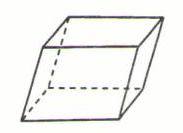
\includegraphics[width=0.2\textwidth]{bodyxb/src/bo_d20aucref24c73anc48g_175_682_968_183_133_0.jpg}  & (1)相对的面是全等的平行四边形； (2)对角面是平行四边形. \\
\cline{1-4}
直平行 六面体 & 侧棱垂直于底的平行 六面体. &  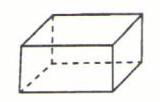
\includegraphics[width=0.2\textwidth]{bodyxb/src/bo_d20aucref24c73anc48g_175_694_1137_160_102_0.jpg}  & (1)侧面、对角面都是矩形； (2)底面是平行四边形. \\
\cline{1-4}
长方体 & 底面是矩形的直平行 六面体. &  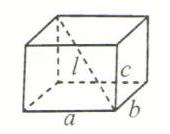
\includegraphics[width=0.2\textwidth]{bodyxb/src/bo_d20aucref24c73anc48g_175_690_1273_170_134_0.jpg}  & (1)六个面、对角面都是矩形； (2) ${l}^{2} = {a}^{2} + {b}^{2} + {c}^{2}$ ; (3) ${S}_{\text{ 全 }} = 2\left( {{ab} + {bc} + {ca}}\right)$ . \\
\cline{1-4}
正四棱柱 & 底面是正方形的长 方体. &  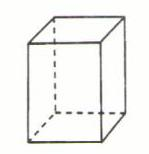
\includegraphics[width=0.2\textwidth]{bodyxb/src/bo_d20aucref24c73anc48g_175_700_1446_149_154_0.jpg}  & (1)侧面、对角面都是矩形； (2)底面是正方形. \\
\cline{1-4}
正方体 & 三度(长、宽、高)相等 的长方体. &  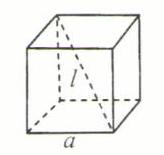
\includegraphics[width=0.2\textwidth]{bodyxb/src/bo_d20aucref24c73anc48g_175_694_1634_164_155_0.jpg}  & (1)六个面都是全等的正方形； (2) $l = \sqrt{3}a;{S}_{\text{ 全 }} = 6{a}^{2}$ . \\
\cline{1-4}
\hline
\end{tabular}
}
\end{center}

例 1 在平行六面体 ${ABCD} - {A}_{1}{B}_{1}{C}_{1}{D}_{1}$ 中 (如图 1(1)) 中,求证:

(1)平面 ${A}_{1}{BD}//$ 平面 ${B}_{1}C{D}_{1}$ ；

(2)对角线 $A{C}_{1}$ 过 $\bigtriangleup  {A}_{1}{BD}$ 的重心,且 $A{C}_{1}$ 被截面 ${A}_{1}{BD},{B}_{1}C{D}_{1}$ 三等分.

证明(1)显然,对角面 ${A}_{1}{B}_{1}{CD}$ 是平行四边形, $\therefore {A}_{1}D//{B}_{1}C,{A}_{1}D$ 不在平面 ${B}_{1}C{D}_{1}$ 上, ${B}_{1}C$ 在平面 ${B}_{1}C{D}_{1}$ 上,

$\therefore A{D}_{1}//$ 平面 ${B}_{1}C{D}_{1}$ .

同理 ${A}_{1}B//$ 平面 ${B}_{1}C{D}_{1}$ ,又 ${A}_{1}B \cap  {A}_{1}D = {A}_{1}$ ,

$\therefore$ 平面 ${A}_{1}{BD}//$ 平面 ${B}_{1}C{D}_{1}$ .

( 2 )连接 ${AC}$ , ${A}_{1}{C}_{1}$ 和 ${BD}$ , ${B}_{1}{D}_{1}$ ,分别交于点 $E$ , ${E}_{1}$ ,连接 ${A}_{1}E$ , ${E}_{1}C$ ,显然, ${A}_{1}E$ , ${E}_{1}C$ 是对角面 $A{A}_{1}{C}_{1}C$ 和平行截面 ${A}_{1}{BD},{B}_{1}C{D}_{1}$ 的交线,故 ${A}_{1}E//{E}_{1}C$ .

\begin{center}
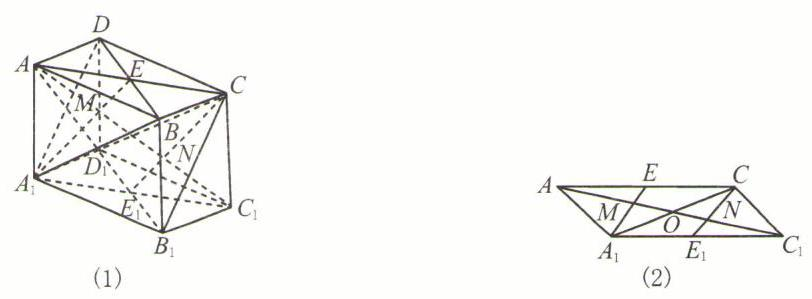
\includegraphics[width=0.6\textwidth]{bodyxb/src/bo_d20aucref24c73anc48g_176_409_384_812_299_0.jpg}
\end{center}


(图 1)

设 $A{C}_{1}$ 和两截面分别交于点 $M,N$ ,则 $M,N$ 必在对角面 $A{A}_{1}{C}_{1}C$ 和截面的交线上,即 $M \in  {A}_{1}E,N \in  {E}_{1}C$ (如图 1(2)),连接 ${A}_{1}C$ ,交 $A{C}_{1}$ 于点 $O$ ,在 $\bigtriangleup A{A}_{1}C$ 中, ${AO},{A}_{1}E$ 是中线, 故 $M$ 是 $\bigtriangleup A{A}_{1}C$ 的重心,则 ${A}_{1}M = {2ME}$ ,故 $M$ 是 $\bigtriangleup {A}_{1}{BD}$ 的重心. 由 ${AM} = {2MO},{C}_{1}N =$  ${2NO}$ 和 ${AO} = {CO}$ ,易知 $M$ , $N$ 三等分 $A{C}_{1}$ .

2. 长方体.

在平行六面体中, 长方体的地位更为特殊: 首先, 长方体的对角线与各棱、各表面的关系有研究的价值; 其次, 有些问题常常可以通过构造长方体来解.

例 2 在长方体 ${ABCD} - {A}_{1}{B}_{1}{C}_{1}{D}_{1}$ 中 (如图 2),

\begin{center}
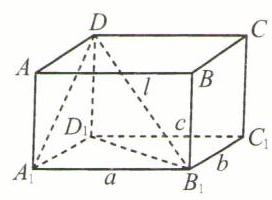
\includegraphics[width=0.2\textwidth]{bodyxb/src/bo_d20aucref24c73anc48g_176_1196_1135_272_200_0.jpg}
\end{center}


(图 2)

(1)设直线 $D{B}_{1}$ 与自 ${B}_{1}$ 出发的三条棱所在直线分别成 $\alpha ,\beta ,\gamma$ 角, 求证: ${\sin }^{2}\alpha  + {\sin }^{2}\beta  + {\sin }^{2}\gamma  = 2$ ;

(2)设 $D{B}_{1}$ 与自 ${B}_{1}$ 出发的三个表面分别成 $\alpha ,\beta ,\gamma$ 角,求证: ${\sin }^{2}\alpha  +$  ${\sin }^{2}\beta  + {\sin }^{2}\gamma  = 1$ .

证明(1)连接 ${A}_{1}D$ ,不妨设 $\angle D{B}_{1}{A}_{1} = \alpha ,\angle D{B}_{1}{C}_{1} = \beta ,\angle D{B}_{1}B = \gamma$ ,长方体的三条棱长分别为 $a,b,c,D{B}_{1} = l$ ,则 ${\sin }^{2}\alpha  = \dfrac{{b}^{2} + {c}^{2}}{{l}^{2}}$ .

同理, ${\sin }^{2}\beta  = \dfrac{{c}^{2} + {a}^{2}}{{l}^{2}},{\sin }^{2}\gamma  = \dfrac{{a}^{2} + {b}^{2}}{l}$ .

$\therefore {\sin }^{2}\alpha  + {\sin }^{2}\beta  + {\sin }^{2}\gamma  = \dfrac{2\left( {{a}^{2} + {b}^{2} + {c}^{2}}\right) }{{l}^{2}} = \dfrac{2{l}^{2}}{{l}^{2}} = 2$ .

(2)连接 ${D}_{1}{B}_{1}$ ,不妨设 $\angle D{B}_{1}{D}_{1} = \alpha ,\angle D{B}_{1}C = \beta ,\angle D{B}_{1}A = \gamma$ ,则 ${\sin }^{2}\alpha  = \dfrac{{c}^{2}}{{l}^{2}}$ .

同理, ${\sin }^{2}\beta  = \dfrac{{a}^{2}}{{l}^{2}},{\sin }^{2}\gamma  = \dfrac{{b}^{2}}{{l}^{2}}$ ,

$\therefore {\sin }^{2}\alpha  + {\sin }^{2}\beta  + {\sin }^{2}\gamma  = \dfrac{{a}^{2} + {b}^{2} + {c}^{2}}{{l}^{2}} = \dfrac{{l}^{2}}{{l}^{2}} = 1$ .

例 3 已知平面 ${OAB},{OBC},{OCA}$ 两两互相垂直,点 $P$ 到上述三个平面的距离分别为 3, 4,5,求点 $P$ 和点 $O$ 间的距离.

解 如图 3,以点 $P$ 和点 $O$ 作为对角线的相对顶点,构造长方体,点 $P$ 到三个面的距离即为此长方体三度的长,所以 ${PO} = \sqrt{{3}^{2} + {4}^{2} + {5}^{2}} = 5\sqrt{2}$ .

\begin{center}
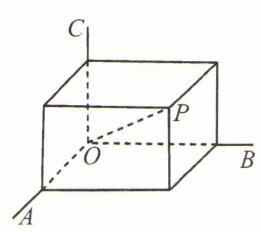
\includegraphics[width=0.2\textwidth]{bodyxb/src/bo_d20aucref24c73anc48g_177_1168_151_261_232_0.jpg}
\end{center}


(图 3)

例 4 四棱柱 ${ABCD} - {A}_{1}{B}_{1}{C}_{1}{D}_{1}$ 的底面是边长为 $a$ 的正方形,侧棱长为 $b\left( {0 < a < \sqrt{2}b}\right)$ ,上底一个顶点 ${A}_{1}$ 与下底面四个顶点等距离(如图 4).

(1)求证:两个对角面一个是矩形,一个垂直于底面,且两个对角面互相垂直;

\begin{center}
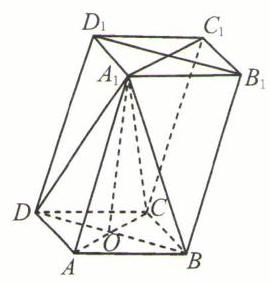
\includegraphics[width=0.2\textwidth]{bodyxb/src/bo_d20aucref24c73anc48g_177_1158_517_270_283_0.jpg}
\end{center}


(图 4)

(2)求两对角面的面积.

(1)证明 作 ${A}_{1}O \bot$ 底面 ${ABCD}$ , $O$ 为垂足.

$\because$ 点 ${A}_{1}$ 到点 $A,B,C,D$ 等距离,

$\therefore O$ 为正方形 ${ABCD}$ 的中心,于是对角面 ${A}_{1}{AC}{C}_{1} \bot$ 底面 ${ABCD}$ .

$\because {DO} \bot  {OC},{DO} \bot  {A}_{1}O$ ,且 ${OC},{A}_{1}O$ 相交,

$\therefore {DO} \bot$ 对角面 ${A}_{1}{AC}{C}_{1}$ ,于是 ${DO} \bot  {A}_{1}A$ ,而 ${D}_{1}D//{A}_{1}A$ ,

$\therefore {DO} \bot  {D}_{1}D$ ,即对角面 ${B}_{1}{BD}{D}_{1}$ 是矩形.

由于 ${DO} \bot$ 对角面 ${A}_{1}{AC}{C}_{1}$ ,又 ${DO} \subset$ 面 ${B}_{1}{BD}{D}_{1}$ ,所以对角面 ${B}_{1}{BD}{D}_{1} \bot$ 对角面 ${A}_{1}{AC}{C}_{1}$ .

(2)解 显然 ${S}_{\text{ 四边形 }{B}_{1}{BD}{D}_{1}} = {BD} \cdot  D{D}_{1} = \sqrt{2}{ab}$ .

$\because {A}_{1}O = \sqrt{{A}_{1}{A}^{2} - A{O}^{2}} = \sqrt{{b}^{2} - \dfrac{{a}^{2}}{2}}$ ,

$\therefore {S}_{\text{ 四边形 }{A}_{1}{AC}{C}_{1}} = {AC} \cdot  {A}_{1}O = \sqrt{2}a \cdot  \sqrt{{b}^{2} - \dfrac{{a}^{2}}{2}} = a\sqrt{2{b}^{2} - {a}^{2}}$ .

\section*{【训练题】}

\section*{(A)}

1. 设 $A = \{$ 直平行六面体 $\} ,B = \{$ 长方体 $\} ,C = \{$ 正四棱柱 $\} ,D = \{$ 直四棱柱 $\}$ ,那么这些集合之间的关系是(   )

(A) $A \supset  D \supset  C \supset  B$ . (B) $D \supset  A \supset  B \supset  C$ .

(C) $D \supset  A \supset  C \supset  B$ . (D) $A \supset  D \supset  B \supset  C$ .

2. 下列结论中, 正确的是 (   )

(A) 直平行六面体是长方体. (B) 对角面为矩形的棱柱是正棱柱.

(C) 侧面都为长方形的棱柱是长方体. (D) 底面为矩形的直棱柱是长方体.

3. 已知 ${EFGH} - {E}_{1}{F}_{1}{G}_{1}{H}_{1}$ 是所有棱长都相等的平行六面体,且 $\angle {E}_{1}{EF} = \angle {E}_{1}{EH} =$  $\angle {FEH} = {60}^{ \circ  }$ ,则对角面 ${F}_{1}{FH}{H}_{1}$ 一定是(   )

(A) 平行四边形但不是菱形. (B) 矩形但不是正方形.

(C) 菱形但不是正方形. (D) 正方形.

4. 底面边长分别是 $a,b$ ,侧棱长为 $c$ 的直平行六面体的侧面积是(   )

(A) ${ac} + {bc}$ . (B) ${2c}\left( {a + b}\right)$ . (C) $2\left( {{ab} + {bc} + {ca}}\right)$ . (D) ${abc}$ .

5. 若一个长方体中共顶点的三个表面的对角线长分别为 $a,b,c$ ,则长方体的对角线长是(   )

(A) $\sqrt{{a}^{2} + {b}^{2} + {c}^{2}}$ . (B) $\sqrt{\dfrac{{a}^{2} + {b}^{2} + {c}^{2}}{2}}$ . (C) $\sqrt{{ab} + {bc} + {ca}}$ . (D) $\sqrt{\dfrac{3\left( {{ab} + {bc} + {ca}}\right) }{2}}$ .

6. 过正三棱柱底面一边和两底中心连线段的中点作截面,则这个截面的形状是(   )

(A) 等腰三角形. (B) 直角三角形. (C) 等腰梯形. (D) 平行四边形.

7. 若正四棱柱的底面边长为 $a$ ,侧面的对角线长为 $b$ ,则正四棱柱的对角线长为 (   )

(A) $\sqrt{{b}^{2} - {a}^{2}}$ . (B) $\sqrt{{a}^{2} + {b}^{2}}$ . (C) $\sqrt{2{a}^{2} + {b}^{2}}$ . (D) $\sqrt{{a}^{2} + 2{b}^{2}}$ .

8. 已知直三棱柱 ${MNP} - {M}_{1}{N}_{1}{P}_{1}$ 的底面 ${MNP}$ 是直角三角形,其中 $\angle {MPN} = {90}^{ \circ  }$ . 记 $\angle {M}_{1}{NM} = \theta ,\angle {NMP} = \alpha ,\angle N{M}_{1}P = \beta$ ,则 $\alpha ,\beta ,\theta$ 间一定有关系式 (   )

(A) $\sin \alpha  = \cos \theta  \cdot  \sin \beta$ . (B) $\sin \beta  = \cos \theta  \cdot  \sin \alpha$ .

(C) $\cos \alpha  = \cos \theta  \cdot  \cos \beta$ . (D) $\cos \beta  = \cos \theta  \cdot  \cos \alpha$ .

9. 已知 $P$ 是单位正方体 ${EFGH} - {E}_{1}{F}_{1}{G}_{1}{H}_{1}$ 的对角线 $F{H}_{1}$ 上的点,且 ${FP} : P{H}_{1} = 1 : 5$ . 过 $P$ 作垂直于 $F{H}_{1}$ 的截面,则这个截面的面积等于 (   )

(A) $\dfrac{\sqrt{3}}{4}$ . (B) $\dfrac{\sqrt{3}}{8}$ . (C) $\dfrac{\sqrt{3}}{16}$ . (D) $\dfrac{\sqrt{3}}{32}$ .

10. (1)若长方体的对角线长为 $\sqrt{14}$ ,所有棱长之和为 24,则长方体的全面积是\blkda{}. ；

(2)若长方体的全面积为 ${22}{\mathrm{{cm}}}^{2}$ ,所有棱的总长度之和为 ${24}\mathrm{{cm}}$ ,则对角线的长度是\blkda{}cm;

(3)已知长方体的长、宽、高之比为 $4 : 3 : {12}$ ,对角线长为 ${26}\mathrm{{cm}}$ ,则它的长、宽、高分别为\blkda{}cm、\blkda{}cm、\blkda{}cm；

(4)若长方体的三个面的面积分别为 $\sqrt{2},\sqrt{3},\sqrt{6}$ ,则长方体的对角线长为\blkda{}.

11. (1) 已知正三棱柱的每条棱长都是 $a$ ,过下底面一边和相对侧棱的上端点作截面,则截面面积为\blkda{}；

(2)已知正三棱柱的底面边长为 $4\mathrm{{cm}}$ ,过下底一边的一个截面与底面成 ${60}^{ \circ  }$ 角,且交相对侧棱于一点,则截面三角形的面积是\blkda{} ${\mathrm{{cm}}}^{2}$ ；

(3)在直三棱柱 ${ABC} - {A}_{1}{B}_{1}{C}_{1}$ 中,底面 $\bigtriangleup  {ABC}$ 是等腰直角三角形, $\angle {ACB} = {90}^{ \circ  }$ ,且腰长与侧棱长相等,则直线 $A{B}_{1}$ 与 ${A}_{1}C$ 所成的角等于\blkda{}；

(4)用一张长、宽分别为 $8\mathrm{{cm}}$ 和 $4\mathrm{{cm}}$ 的矩形硬纸折成正四棱柱的侧面,则此正四棱柱的对角线长为\blkda{} $\mathrm{{cm}}$ ；

(5)设正四棱柱 ${ABCD} - {A}_{1}{B}_{1}{C}_{1}{D}_{1}$ 的底面边长为 $a$ ,侧棱长为 ${2a}$ ,则顶点 ${B}_{1}$ 到截面 ${A}_{1}B{C}_{1}$ 的距离为\blkda{}；

(6)正六棱柱的各条棱长都是 $a$ ,则其对角面的面积等于\blkda{}.

12. (1) 若底面为菱形的直棱柱的两条对角线长分别为 $9\mathrm{{cm}}$ 和 ${15}\mathrm{{cm}}$ ,侧棱长为 $5\mathrm{{cm}}$ ,求此直棱柱的底面边长;

(2)已知直平行六面体的底面是菱形,过不相邻的两对侧棱的截面面积分别是 $3{\mathrm{{cm}}}^{2}$ 和 $4{\mathrm{{cm}}}^{2}$ ,求此直平行六面体的侧面积;

(3)在底面是边长为 $8\mathrm{{cm}}$ 的菱形的直棱柱中,若对角面的面积分别为 ${50}\sqrt{2}{\mathrm{{cm}}}^{2}$ 和 ${10}\sqrt{14}{\mathrm{{cm}}}^{2}$ ,求直棱柱的对角线长；

(4)在直平行六面体 ${ABCD} - {A}_{1}{B}_{1}{C}_{1}{D}_{1}$ 中,已知 ${AB} = 5,{AD} = 3,{A{A}_{1}} = 4,\angle {DAB} =$  ${60}^{ \circ  }$ ,求对角线 $A{C}_{1}$ 和 $B{D}_{1}$ 的长;

(5)已知长方体 ${ABCD} - {A}_{1}{B}_{1}{C}_{1}{D}_{1}$ 的对角线长为 $l$ ,对角线 $B{D}_{1}$ 与底面 ${ABCD}$ 、侧面 ${B}_{1}{BC}{C}_{1}$ 分别成 ${45}^{ \circ  }$ 和 ${30}^{ \circ  }$ 角,求此长方体的全面积.

13. 在各棱长均为 1 的正三棱柱 ${ABC} - {A}_{1}{B}_{1}{C}_{1}$ 中,

(1)求面对角线 $B{C}_{1}$ 与侧面 ${AB}{B}_{1}{A}_{1}$ 所成角的正切值(如图)；

\begin{center}
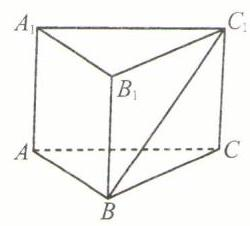
\includegraphics[width=0.2\textwidth]{bodyxb/src/bo_d20aucref24c73anc48g_179_420_807_250_226_0.jpg}
\end{center}


[第 13(1)题]

\begin{center}
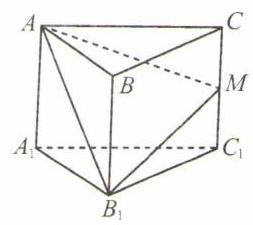
\includegraphics[width=0.2\textwidth]{bodyxb/src/bo_d20aucref24c73anc48g_179_934_805_253_225_0.jpg}
\end{center}


[第 13(2)题]

(2)如果 $M$ 为 $C{C}_{1}$ 的中点,求平面 $A{B}_{1}M$ 与底面 ${A}_{1}{B}_{1}{C}_{1}$ 所成锐二面角的大小(如图).

\section*{(B)}

14. 若一个平行六面体的各个侧面都是正方形, 则这个平行六面体一定是 (   )

(A) 正方体. (B) 直平行六面体. (C) 长方体. (D) 正四棱柱.

15. 若一个平行六面体的两个对角面都是矩形, 给出以下四个结论: ①这个平行六面体一定是直平行六面体；②这个平行六面体有可能是斜平行六面体；③这个平行六面体有可能是正四棱柱；④这个平行六面体不可能是正方体. 其中正确的个数是(   )

(A) 1 . (B) 2 . (C) 3. (D) 4.

16. 在正方体的八个顶点中, 有四个恰好是正四面体的顶点, 则正方体的全面积与正四面体的全面积之比为(   )

(A) $\sqrt{2}$ . (B) $\sqrt{3}$ . (C) $\dfrac{\sqrt{6}}{2}$ . (D) $\dfrac{\sqrt{6}}{3}$ .

17. 若长方体的对角线与交于一点的三个面所成的角分别为 $\alpha ,\beta ,\gamma$ ,则有 (   )

(A) ${\sin }^{2}\alpha  + {\sin }^{2}\beta  + {\sin }^{2}\gamma  = 2$ . (B) ${\cos }^{2}\alpha  + {\cos }^{2}\beta  + {\cos }^{2}\gamma  = 2$ .

(C) ${\cos }^{2}\alpha  + {\cos }^{2}\beta  + {\cos }^{2}\gamma  = 1$ . (D) ${\tan }^{2}\alpha  + {\tan }^{2}\beta  + {\tan }^{2}\gamma  = 1$ .

18. 已知平面 $\alpha ,\beta ,\gamma$ 两两互相垂直,它们的三条交线的公共点为 $O$ ,过 $O$ 引一条射线 ${OP}$ . 若 ${OP}$ 与三条交线中的两条所成的角都是 ${60}^{ \circ  }$ ,则 ${OP}$ 与第三条交线所成的角为(   )

(A) ${30}^{ \circ  }$ . (B) ${45}^{ \circ  }$ . (C) ${60}^{ \circ  }$ . (D) ${75}^{ \circ  }$ .

19. 已知正方体 ${ABCD} - {A}_{1}{B}_{1}{C}_{1}{D}_{1}$ 的棱长为 $1,P$ 是 $A{A}_{1}$ 的中点, $E$ 是 $B{B}_{1}$ 上一点,则 ${PE} +$  ${EC}$ 的最小值是 (   )

(A) 2 . (B) $\dfrac{\sqrt{15}}{2}$ . (C) $\dfrac{\sqrt{17}}{2}$ . (D) $\sqrt{3}$ .

20. 已知三棱柱的底面是边长为 5 的等边三角形,其中一条侧棱与底面的两边都成 ${60}^{ \circ  }$ 角,侧棱长为 4 , 则三棱柱的侧面积为 (   )

(A) ${30}\sqrt{3}$ . (B) ${50}\left( {\sqrt{3} + 1}\right)$ . (C) ${40}\left( {\sqrt{3} + 1}\right)$ . (D) ${20}\left( {\sqrt{3} + 1}\right)$ .

21. 在底面边长为 $a$ 的正三棱柱 ${ABC} - {A}_{1}{B}_{1}{C}_{1}$ 中, $D,E$ 分别为侧棱 $B{B}_{1},C{C}_{1}$ 上的点,且 ${EC} = {BC} = {2BD}$ (如图). 求:

\begin{center}
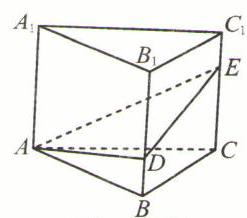
\includegraphics[width=0.2\textwidth]{bodyxb/src/bo_d20aucref24c73anc48g_180_1245_544_247_218_0.jpg}
\end{center}


(第 21 题)

(1)平面 ${ADE}$ 与平面 ${ABC}$ 所成锐二面角的大小；

(2)点 $C$ 到截面 ${ADE}$ 的距离.

22. (1) 在斜三棱柱 ${ABC} - {A}_{1}{B}_{1}{C}_{1}$ 中,底面是边长为 $a$ 的正三角形,侧棱长为 $b$ ,一条侧棱与底面内相邻两边所夹的角都为 ${45}^{ \circ  }$ ,求它的侧面积;

(2)已知斜三棱柱 ${ABC} - {A}_{1}{B}_{1}{C}_{1}$ 各条棱长都是 $a$ ,且 ${A}_{1}A = {A}_{1}B = {A}_{1}C$ (如图),求此三棱柱的全面积;

\begin{center}
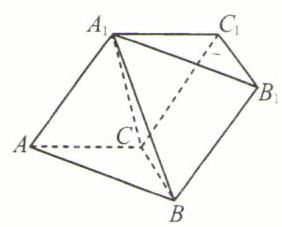
\includegraphics[width=0.2\textwidth]{bodyxb/src/bo_d20aucref24c73anc48g_180_457_1042_282_227_0.jpg}
\end{center}


[第 22(2)题]

\begin{center}
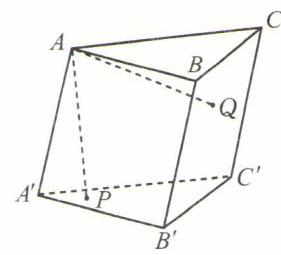
\includegraphics[width=0.2\textwidth]{bodyxb/src/bo_d20aucref24c73anc48g_180_1000_1014_281_255_0.jpg}
\end{center}


[第 22(3)题]

(3)已知三棱柱 ${ABC} - {A}^{\prime }{B}^{\prime }{C}^{\prime }$ 的底面是边长为 $a$ 的正三角形, $\angle A{A}^{\prime }{B}^{\prime } = \angle A{A}^{\prime }{C}^{\prime } =$  ${45}^{ \circ  }$ ,顶点 $A$ 到底面 ${A}^{\prime }{B}^{\prime }{C}^{\prime }$ 和侧面 $B{B}^{\prime }{C}^{\prime }C$ 等距离 (如图),求该三棱柱的侧面积.

23. 在底面为菱形的平行六面体 ${ABCD} - {A}_{1}{B}_{1}{C}_{1}{D}_{1}$ 中 (如图),若 $\angle {A}_{1}{AB} = \angle {A}_{1}{AD}$ ,求证: 平行六面体的一个对角面垂直于底面,另一个对角面是矩形,且两对角面互相垂直.

\begin{center}
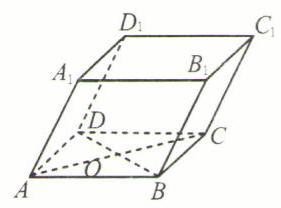
\includegraphics[width=0.2\textwidth]{bodyxb/src/bo_d20aucref24c73anc48g_180_430_1616_281_208_0.jpg}
\end{center}


(第 23 题)

\begin{center}
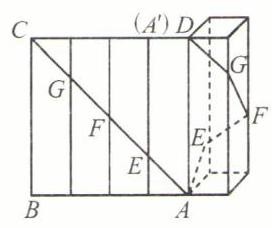
\includegraphics[width=0.2\textwidth]{bodyxb/src/bo_d20aucref24c73anc48g_180_974_1595_272_228_0.jpg}
\end{center}


(第 24 题)

24. 将正方形 ${ABCD}$ 折成一个正四棱柱的四个侧面,则原对角线 ${AC}$ 成了一条绕在正四棱柱上的折线 ${AEFG}{A}^{\prime }$ . 求:

(1)折线 ${AEFG}{A}^{\prime }$ 相邻两线段间的夹角；

(2)异面直线 ${A}^{\prime }G$ 和 ${EF}$ 所成的角；

(3)异面直线 ${A}^{\prime }G$ 和 ${AE}$ 所成的角.

25. (1) 已知直三棱柱 ${ABC} - {A}_{1}{B}_{1}{C}_{1}$ 的侧棱长为 $a$ ,底面为直角三角形, ${AC} = {BC} = a,\angle {ACB} = {90}^{ \circ  }$ (如图),求平面 ${A}_{1}{AB}{B}_{1}$ 与平面 $A{B}_{1}C$ 所成锐二面角的大小;

\begin{center}
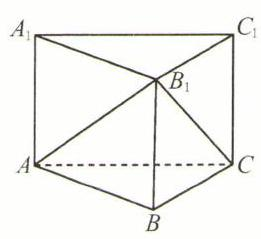
\includegraphics[width=0.2\textwidth]{bodyxb/src/bo_d20aucref24c73anc48g_181_1161_150_261_239_0.jpg}
\end{center}


[第 25(1)题]

(2)已知正三棱柱 ${ABC} - {A}_{1}{B}_{1}{C}_{1}$ 的棱长都为 $a$ ,过底面一边和两底中心连线的中点作截面, 求截面面积.

26. 在正三棱柱 ${ABC} - {A}_{1}{B}_{1}{C}_{1}$ 中,

(1)若 $A{B}_{1}\bot B{C}_{1}$ (如图),求证: $A{B}_{1}\bot {A}_{1}C$ ；

\begin{center}
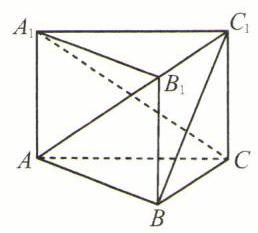
\includegraphics[width=0.2\textwidth]{bodyxb/src/bo_d20aucref24c73anc48g_181_416_554_258_233_0.jpg}
\end{center}


[第 26(1)题]

\begin{center}
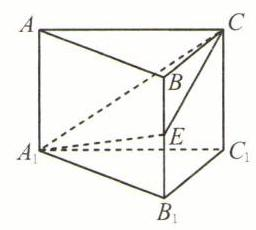
\includegraphics[width=0.2\textwidth]{bodyxb/src/bo_d20aucref24c73anc48g_181_930_555_256_230_0.jpg}
\end{center}


[第 26(2)题]

(2)若 $E$ 在侧棱 $B{B}_{1}$ 上,截面 ${A}_{1}{EC} \bot$ 侧面 $A{C}_{1}$ (如图).

① 求证: ${BE} = {E{B}_{1}}$ ；

②若 $A{A}_{1} = {A}_{1}{B}_{1}$ ,求平面 ${A}_{1}{EC}$ 与平面 ${A}_{1}{B}_{1}{C}_{1}$ 所成二面角 (锐角) 的度数.

27. 在底面为等腰直角三角形的直三棱柱 ${ABC} - {A}_{1}{B}_{1}{C}_{1}$ 中, $\angle {ACB} = {90}^{ \circ  },{AC} = {BC} = A{A}_{1} =$  $a$ (如图).

(1)求 $A{B}_{1}$ 与 $B{C}_{1}$ 所成的角；

(2)若点 $E$ 为 ${AB}$ 的中点,求 ${CE}$ 与 $B{C}_{1}$ 所成的角；

(3)求二面角 ${A}_{1} - A{B}_{1} - {C}_{1}$ 的大小.

\begin{center}
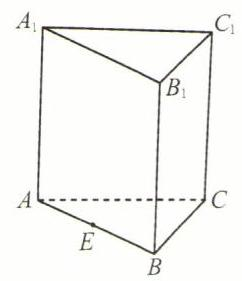
\includegraphics[width=0.2\textwidth]{bodyxb/src/bo_d20aucref24c73anc48g_181_365_1335_242_281_0.jpg}
\end{center}


(第 27 题)

\begin{center}
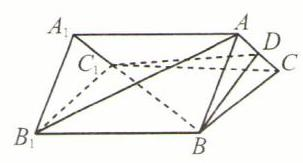
\includegraphics[width=0.2\textwidth]{bodyxb/src/bo_d20aucref24c73anc48g_181_867_1453_303_163_0.jpg}
\end{center}


(第 29 题)

28. 正三棱柱 ${ABC} - {A}_{1}{B}_{1}{C}_{1}$ 的底面边长为 3,侧棱长为 $3\sqrt{2}$ ,求过 $A{B}_{1}$ 且平行于 $B{C}_{1}$ 的截面与底面所成角的正切值.

29. 在正三棱柱 ${A}_{1}{B}_{1}{C}_{1} - {ABC}$ 中,已知 $D$ 是 ${AC}$ 的中点 (如图).

(1)求证: $A{B}_{1}//$ 平面 ${DB}{C}_{1}$ ；

(2)若 $A{B}_{1} \bot  B{C}_{1},{BC} = 2$ ,求线段 $A{B}_{1}$ 在侧面 ${B}_{1}{BC}{C}_{1}$ 上的射影长；

(3)若 $A{B}_{1} \bot  B{C}_{1}$ ,求二面角 $D - B{C}_{1} - C$ 的大小.

\section*{(二) 棱锥}

\section*{【典型题型和解题技巧】}

\section*{1. 正棱锥中的角.}

(1)侧棱与底面所成的角.

\begin{center}
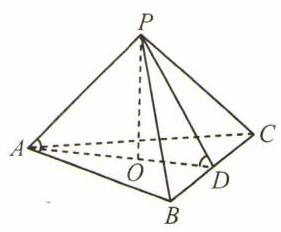
\includegraphics[width=0.2\textwidth]{bodyxb/src/bo_d20aucref24c73anc48g_182_1242_451_281_232_0.jpg}
\end{center}


(图 5)

正棱锥中侧棱与底面所成的角, 就是侧棱与侧棱在底面上的射影 (即底面正多边形外接圆的一条半径)的夹角,如图 5 ,以正三棱锥 $P - {ABC}$ 为例, ${PO}$ 是高,侧棱 ${PA}$ 与底面所成的角就是 $\angle {PAO}$ .

(2)侧面与底面所成的角.

正棱锥侧面与底面所成的角就是它的斜高与斜高在底面上的射影 (即底面正多边形内切圆的一条半径) 的夹角. 如图 5, ${PD}$ 是正三棱锥的斜高,侧面 ${PBC}$ 与底面 ${ABC}$ 所成的角就是 $\angle {PDO}$ .

(3)相邻侧面所成的角.

正棱锥中相邻侧面所成的角,因正棱锥的分类不同而略有差异.

如图 6,在正三棱锥 $P - {ABC}$ 中,显然,由于 ${PA} \bot  {BC}$ ,故可过 ${BC}$ 作 ${PA}$ 的垂面交 ${PA}$ 于点 $M$ ,则 $\angle {BMC}$ 就是相邻侧面 ${PAB}$ 和 ${PAC}$ 所成二面角的平面角;

如图 7,在正四棱锥 $P - {ABCD}$ 中,由于 ${PC} \bot  {BD}$ ,故可过 ${BD}$ 作 ${PC}$ 的垂面交 ${PC}$ 于点 $N$ ,则 $\angle {BND}$ 就是相邻侧面 ${PCB}$ 和 ${PCD}$ 所成二面角的平面角;

\begin{center}
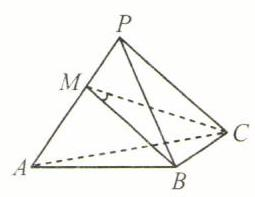
\includegraphics[width=0.2\textwidth]{bodyxb/src/bo_d20aucref24c73anc48g_182_374_1283_255_197_0.jpg}
\end{center}


(图 6)

\begin{center}
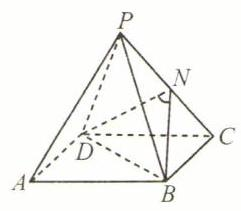
\includegraphics[width=0.2\textwidth]{bodyxb/src/bo_d20aucref24c73anc48g_182_759_1269_241_211_0.jpg}
\end{center}


(图 7)

\begin{center}
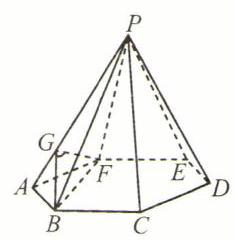
\includegraphics[width=0.2\textwidth]{bodyxb/src/bo_d20aucref24c73anc48g_182_1128_1236_234_241_0.jpg}
\end{center}


(图 8)

如图 8,在正六棱锥 $P - {ABCDEF}$ 中,由于 ${PA} \bot  {BF}$ ,故可过 ${BF}$ 作 ${PA}$ 的垂面交 ${PA}$ 于点 $G$ ,则 $\angle {BGF}$ 就是相邻侧面 ${PAB}$ 和 ${PAF}$ 所成二面角的平面角.

在解正棱锥问题时,如果能够熟练使用正多边形的边长 $a$ 与外接圆半径 $R$ 、内切圆半径 $r$ 和面积 $S$ 之间的关系,将会给计算带来很大的便利. 如下表:

\begin{center}
\adjustbox{width=\textwidth}{
\begin{tabular}{|c|c|c|c|c|}
\hline
\phantom{X} & 图 形 & $R$ & $r$ & $S$ \\
\cline{1-5}
正三角形 &  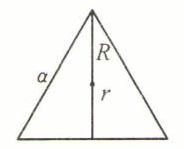
\includegraphics[width=0.2\textwidth]{bodyxb/src/bo_d20aucref24c73anc48g_182_577_1865_184_149_0.jpg}  & $\dfrac{\sqrt{3}}{3}a$ & $\dfrac{\sqrt{3}}{6}a$ & $\dfrac{\sqrt{3}}{4}{a}^{2}$ \\
\cline{1-5}
\hline
\end{tabular}
}
\end{center}

续表

\begin{center}
\adjustbox{width=\textwidth}{
\begin{tabular}{|c|c|c|c|c|}
\hline
\phantom{X} & 图 形 & $R$ & $r$ & $S$ \\
\cline{1-5}
正方形 &  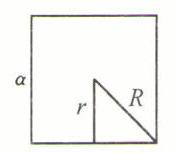
\includegraphics[width=0.2\textwidth]{bodyxb/src/bo_d20aucref24c73anc48g_183_500_264_177_153_0.jpg}  & $\dfrac{\sqrt{2}}{2}a$ & $\dfrac{a}{2}$ & ${a}^{2}$ \\
\cline{1-5}
正六边形 &  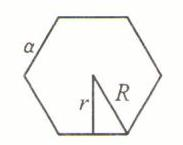
\includegraphics[width=0.2\textwidth]{bodyxb/src/bo_d20aucref24c73anc48g_183_494_446_183_145_0.jpg}  & $a$ & $\dfrac{\sqrt{3}}{2}a$ & $\dfrac{3\sqrt{3}}{2}{a}^{2}$ \\
\cline{1-5}
\hline
\end{tabular}
}
\end{center}

例 1 已知正三棱锥 $P - {ABC}$ 的各棱长都相等,求:

(1)侧棱与底面所成角的余弦值；

\begin{center}
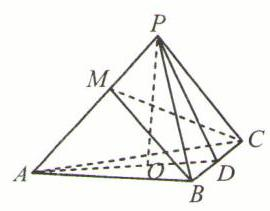
\includegraphics[width=0.2\textwidth]{bodyxb/src/bo_d20aucref24c73anc48g_183_1172_688_270_211_0.jpg}
\end{center}


(图 9)

(2)侧面与底面所成角的正弦值；

( 3 )相邻侧面所成二面角的余弦值.

解 如图 9,记 $P$ 在底面上的射影为 $O,{BC}$ 中点为 $D$ ,再过 ${BC}$ 作 ${PA}$ 的垂面交 ${PA}$ 于点 $M$ ,则 $\angle {PAO},\angle {PDO},\angle {BMC}$ 分别是侧棱与底面、侧面与底面、相邻侧面所成二面角的平面角.

令 ${AB} = 6$ ,则:

(1) ${OA} = 2\sqrt{3},\cos \angle {PAO} = \dfrac{OA}{PA} = \dfrac{2\sqrt{3}}{6} = \dfrac{\sqrt{3}}{3}$ .

(2) ${OD} = \sqrt{3},{PD} = 3\sqrt{3},{PO} = \sqrt{{27} - 3} = 2\sqrt{6},\sin \angle {PDO} = \dfrac{PO}{PD} = \dfrac{2\sqrt{6}}{3\sqrt{3}} = \dfrac{2\sqrt{2}}{3}$ .

(3) ${BM} = {MC} = 3\sqrt{3},{BC} = 6,\cos \angle {BMC} = \dfrac{B{M}^{2} + C{M}^{2} - B{C}^{2}}{{2BM} \cdot  {CM}} = \dfrac{{27} + {27} - {36}}{2 \cdot  3\sqrt{3} \cdot  3\sqrt{3}} = \dfrac{1}{3}$ . 2. 三棱锥顶点在底面上射影的位置.

如图 10,在三棱锥 $P - {ABC}$ 中,顶点 $P$ 在底面上的射影为 $O(O$ 在 $\bigtriangleup  {ABC}$ 内部).

\begin{center}
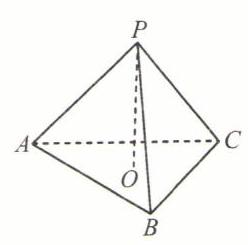
\includegraphics[width=0.2\textwidth]{bodyxb/src/bo_d20aucref24c73anc48g_183_1197_1461_248_245_0.jpg}
\end{center}


(图 10)

容易证明:

(1)若 ${PA} = {PB} = {PC}$ ,或 ${PA},{PB},{PC}$ 与底面成等角,则 $O$ 是 $\bigtriangleup  {ABC}$ 的外心;

(2)若三侧面与底面成等角,或 $P$ 到底面三边等距离,则 $O$ 是 $\bigtriangleup  {ABC}$ 的内心;

(3)若 ${PA},{PB},{PC}$ 两两互相垂直,或有两组对棱互相垂直,则 $O$ 是 $\bigtriangleup  {ABC}$ 的垂心. 例 2 在三棱锥 $P - {ABC}$ 中,已知 ${AB} = 1,{AC} = 2,\angle {BAC}$ 的平分线 ${AD} = 1$ ,且棱锥的三个侧面与底面都成 ${60}^{ \circ  }$ 角 (如图 11),求:

\begin{center}
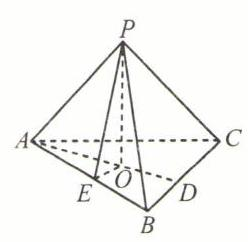
\includegraphics[width=0.2\textwidth]{bodyxb/src/bo_d20aucref24c73anc48g_183_1197_1914_248_242_0.jpg}
\end{center}


(图 11)

(1)三棱锥的侧面积；

(2)三棱锥的高.

解(1)设 $\angle {BAC} = {2\theta }$ ,

则 ${S}_{\bigtriangleup {ABC}} = \dfrac{1}{2}{AB} \cdot  {AC}\sin {2\theta } = \sin {2\theta }$ .

又 ${S}_{\bigtriangleup {ABC}} = {S}_{\bigtriangleup {ABD}} + {S}_{\bigtriangleup {ACD}} = \dfrac{1}{2}\left( {{AB} \cdot  {AD} + {AC} \cdot  {AD}}\right) \sin \theta  = \dfrac{3}{2}\sin \theta$ ,

于是 $2\sin {2\theta } = 3\sin \theta$ ,即 $4\sin \theta \cos \theta  = 3\sin \theta$ .

显然 $\sin \theta  \neq  0,\therefore \cos \theta  = \dfrac{3}{4},\therefore \sin \theta  = \dfrac{\sqrt{7}}{4}$ .

故 ${S}_{\bigtriangleup {ABC}} = \dfrac{3}{2}\sin \theta  = \dfrac{3\sqrt{7}}{8}$ .

$\because$ 三棱锥的三侧面与底面都成 ${60}^{ \circ  }$ 角,

故由 $\cos {60}^{ \circ  } = \dfrac{{S}_{\text{ 底 }}}{{S}_{\text{ 侧 }}}$ ,得 ${S}_{\text{ 侧 }} = 2{S}_{\text{ 底 }} = \dfrac{3\sqrt{7}}{4}$ .

(2)由 $\cos \theta  = \dfrac{3}{4}$ 得 $\cos {2\theta } = 2{\cos }^{2}\theta  - 1 = \dfrac{1}{8}$ ,于是由余弦定理得

$B{C}^{2} = A{B}^{2} + A{C}^{2} - {2AB} \cdot  {AC} \cdot  \cos {2\theta } = 1 + 4 - 2 \cdot  1 \cdot  2 \cdot  \dfrac{1}{8} = \dfrac{9}{2},$

$\therefore {BC} = \dfrac{3\sqrt{2}}{2}$ .

过点 $P$ 作 ${PO} \bot$ 面 ${ABC}$ 于点 $O$ ,则由条件知 $O$ 是 $\bigtriangleup {ABC}$ 的内心,再作 ${OE} \bot  {AB}$ 于点 $E$ , 连接 ${PE}$ ,则由三垂线定理得, ${PE}\bot {AB},\angle {PEO} = {60}^{ \circ  }$ ,且 ${OE}$ 是 $\bigtriangleup {ABC}$ 内切圆的半径,于是

${S}_{\bigtriangleup {ABC}} = \dfrac{1}{2}\left( {{AB} + {AC} + {BC}}\right)  \cdot  {OE} = \dfrac{1}{2}\left( {1 + 2 + \dfrac{3\sqrt{2}}{2}}\right)  \cdot  {OE} = \dfrac{3\sqrt{7}}{8},$

得 ${OE} = \dfrac{\sqrt{14}\left( {\sqrt{2} - 1}\right) }{4}$ ,于是高 ${PO} = {OE} \cdot  \tan {60}^{ \circ  } = \dfrac{\sqrt{42}\left( {\sqrt{2} - 1}\right) }{4}$ .

注意 如果棱锥的各个侧面与底面成等角 $\theta$ ,容易证明: $\cos \theta  = \dfrac{{S}_{\text{ 底 }}}{{S}_{\text{ 侧 }}}$ .

【训练题】

\section*{(A)}

30. 若正三棱锥的侧棱与底面边长相等,则侧棱与底面所成角的余弦值为(   )

(A) $\dfrac{1}{2}$ . (B) $\dfrac{\sqrt{2}}{2}$ . (C) $\dfrac{1}{3}$ . (D) $\dfrac{\sqrt{3}}{3}$ .

31. 若正三棱锥的一个侧面与底面面积之比是 $\dfrac{2}{3}$ ,则此三棱锥的高与斜高之比是 (   )

(A) $\dfrac{\sqrt{3}}{2}$ . (B) $\dfrac{\sqrt{2}}{2}$ . (C) $\dfrac{1}{2}$ . (D) 1 .

32. 若侧面都为直角三角形的正三棱锥的底面边长为 $a$ ,则它的全面积等于(   )

(A) $\dfrac{3 + \sqrt{3}}{4}{a}^{2}$ . (B) $\dfrac{3}{4}{a}^{2}$ .

(C) $\dfrac{3 + \sqrt{3}}{2}{a}^{2}$ . (D) $\dfrac{6 + \sqrt{3}}{4}{a}^{2}$ .

33. 在正三棱锥 $P - {EFG}$ 中,已知底面边长 ${EF}$ 为 $a$ ,侧棱长为 $b$ ,过 ${PE},{PF},{FG}$ 的中点作一截面, 则此截面面积等于 (   )

(A) $\dfrac{1}{4}{ab}$ . (B) $\dfrac{1}{8}{ab}$ .

(C) $\dfrac{\sqrt{2}}{8}{ab}$ . (D) $\dfrac{ab}{4}\sin \theta$ ,其中角 $\theta$ 满足 $\tan \theta  = \dfrac{b}{a}$ .

34. 在棱锥 $P - {ABCD}$ 中,已知底面 ${ABCD}$ 是正方形,两侧面 ${PAD},{PDC}$ 垂直于底面,另两个侧面与底面都成 ${45}^{ \circ  }$ 角,且最长的侧棱长为 15 ,则此棱锥的高等于(   )

(A) 12 . (B) $5\sqrt{3}$ . (C) $6\sqrt{2}$ . (D) $3\sqrt{5}$ .

35. 侧面为正三角形的正四棱锥中,侧面与底面所成二面角的余弦值为(   )

(A) $\dfrac{1}{2}$ . (B) $\dfrac{\sqrt{2}}{2}$ . (C) $\dfrac{\sqrt{3}}{3}$ . (D) $\dfrac{\sqrt{3}}{2}$ .

36. 若一个正四棱锥的中截面面积是 $Q$ ,则它的底面边长是 (   )

(A) $\dfrac{Q}{4}$ . (B) $\dfrac{\sqrt{Q}}{2}$ . (C) $\sqrt{Q}$ . (D) $2\sqrt{Q}$ .

37. 一个 $n$ 棱锥的所有侧面与底面所成的二面角都为 ${30}^{ \circ  }$ ,若此棱锥的底面面积为 $S$ ,则它的侧面积等于(   )

(A) $\dfrac{1}{2}S$ . (B) $\dfrac{\sqrt{3}}{2}S$ . (C) $\dfrac{2\sqrt{3}}{3}S$ . (D) 2S.

38. 若正六棱锥的底面边长为 2 , 高为 1 , 则其顶点到底面各边的距离等于(   )

(A) $\sqrt{6}$ . (B) $\sqrt{5}$ . (C) 2 . (D) $\sqrt{3}$ .

39. 在正三棱锥中,

(1)若底面边长为 $\sqrt{3}$ ,侧棱长为 2,则其高是\blkda{}；

(2)若侧棱长与底面边长之比为 $2 : 3$ ,则高与斜高之比等于\blkda{}；

(3)若底面边长为 $a$ ,侧棱与底面所成的角是 ${45}^{ \circ  }$ ,则斜高等于\blkda{}；

(4)若棱长都是 $a$ ,则以各侧面中心为顶点的三角形面积等于\blkda{}；

(5)若侧棱长为 $\sqrt{5}\mathrm{{cm}}$ ,底面边长为 $2\mathrm{{cm}}$ ,则侧面与底面所成二面角的正弦值为\blkda{}.

40. 已知正三棱台的上、下底面边长分别为 2 与 6,侧面与下底面所成二面角为 ${60}^{ \circ  }$ ,则棱台的高是(   )

(A) $\dfrac{3}{2}$ . (B) 2 . (C) 3. (D) 4 .

41. 已知正三棱台侧面与底面所成的角为 ${\theta }_{1}$ ,侧棱与底面所成的角为 ${\theta }_{2}$ ,则 $\tan {\theta }_{1} : \tan {\theta }_{2}$ 的值是(   )

(A) $\dfrac{1}{2}$ . (B) $\dfrac{1}{3}$ . (C) 2 . (D) 3.

42. 若正四棱台的侧棱与底面所成的角为 ${45}^{ \circ  }$ ,则侧面与底面所成角的正弦值为(   )

(A) $\dfrac{\sqrt{6}}{3}$ . (B) $\dfrac{\sqrt{2}}{4}$ . (C) $\dfrac{\sqrt{2}}{3}$ . (D) $\dfrac{\sqrt{2}}{2}$ .

43. 已知棱台两底面面积分别为 ${49}{\mathrm{{cm}}}^{2}$ 与 ${16}{\mathrm{{cm}}}^{2}$ ,而截得此棱台的原棱锥的高是 ${21}\mathrm{{cm}}$ ,则棱台的高是(   )

(A) ${12}\mathrm{{cm}}$ . (B) $\dfrac{147}{41}\mathrm{{cm}}$ . (C) $\dfrac{84}{41}\mathrm{{cm}}$ . (D) $9\mathrm{{cm}}$ .

44. 已知棱台的中截面面积为 ${64}{\mathrm{{cm}}}^{2}$ ,上底面面积为 ${36}{\mathrm{{cm}}}^{2}$ ,则棱台的下底面面积是(   )

(A) ${80}{\mathrm{{cm}}}^{2}$ . (B) ${92}{\mathrm{{cm}}}^{2}$ . (C) ${100}{\mathrm{{cm}}}^{2}$ . (D) $\dfrac{1024}{9}{\mathrm{{cm}}}^{2}$ .

45. 已知正三棱台的上、下底面边长分别为 2 和 6,侧面与下底面成 ${60}^{ \circ  }$ 角,则棱台的侧面积为(   )

(A) 8 . (B) $8\sqrt{3}$ . (C) 16. (D) ${16}\sqrt{3}$ .

46. (1) 三棱锥 $P - {ABC}$ 的底面为等腰直角三角形,其斜边 ${AC}$ 长为 10,三棱锥的侧棱 ${PA}$ , ${PB},{PC}$ 都等于 13,则顶点 $P$ 到底面 ${ABC}$ 的距离是\blkda{}；

(2)若三棱锥 $P - {ABC}$ 的三个侧面与底面所成的二面角都是 $\beta$ ,它的高是 $h$ ,则这个三棱锥底面内切圆的半径等于\blkda{}；

(3) $E,F$ 分别是单位正方形 ${ABCD}$ 的边 ${BC},{CD}$ 的中点,沿 ${AE},{EF},{AF}$ 将它折成一个四面体 ${PAEF}$ ,使 $B,C,D$ 三点重合于点 $P$ ,则 $P$ 到面 ${AEF}$ 的距离是\blkda{}；

(4)在三棱锥 $P - {ABC}$ 中,已知底面 $\bigtriangleup  {ABC}$ 的三边长分别为7,8,9,且各侧面与底面都成 ${60}^{ \circ  }$ 角,则此三棱锥的侧面积等于\blkda{}.

47. (1) 已知四棱锥 $P - {ABCD}$ 的底面是边长为 1 的正方形,侧棱 ${PB}$ 垂直于底面,并且 ${PB}$  $= \sqrt{3}$ ,则 $\angle {APD}$ 的正弦值等于\blkda{}；

(2)若正四棱锥的底面积为 $Q$ ,侧面积为 $P$ ,则侧面与底面所成角的余弦值为\blkda{}；

(3)已知正四棱锥的侧棱与底面成 ${60}^{ \circ  }$ 角,则此四棱锥的两个相邻侧面所成二面角的余弦值等于\blkda{}.

48. (1) 已知正四棱台底面边长分别为 ${20}\mathrm{{cm}}$ 和 ${40}\mathrm{{cm}}$ ,它的侧面积等于两个底面面积之和, 则它的斜高为\blkda{} $\mathrm{{cm}}$ ,高为\blkda{} $\mathrm{{cm}}$ ；

(2)若正六棱台的上、下底面的边长分别为 $a$ 和 $b\left( {0 < a < b}\right)$ ,侧面和下底面所成的二面角是 ${60}^{ \circ  }$ ,则它的侧面积为\blkda{}；

(3)若正四棱台的高是 ${12}\mathrm{{cm}}$ ,两个底面边长的差是 ${10}\mathrm{{cm}}$ ,全面积是 ${512}{\mathrm{{cm}}}^{2}$ ,则这个正四棱台的侧面积等于\blkda{} ${\mathrm{{cm}}}^{2}$ .

49. (1)已知正三棱台侧面与底面成 ${45}^{ \circ  }$ 角,侧棱与底面成 $\theta$ 角,则 $\tan \theta$ 等于\blkda{}；

(2)若正三棱台的侧棱与底面成 ${45}^{ \circ  }$ 角,则其侧面与底面所成角的余弦值等于\blkda{}；

(3)已知正四棱台的两底面边长分别为 6 和 2,且对角面上两对角线互相垂直,则其侧面积为\blkda{}.

50. (1) 已知正四棱锥底面边长为 ${2a}$ ,侧面与底面成 ${45}^{ \circ  }$ 的二面角,过高的中点作平行于底面的截面,则截得的棱台的全面积为\blkda{}；

(2)一个棱锥的侧面积为 $Q$ ,在高 ${PO}$ 上取一点 $A$ ,使 ${PA} = \dfrac{1}{3}{PO}(P$ 为顶点),过 $A$ 作平行于底面的平面截得一个棱台,则此棱台的侧面积为\blkda{}；

(3)过棱锥高的三等分点作两个平行于底面的截面,则该棱锥侧面被这两个截面分成的三部分(自顶点到底面)的面积之比是\blkda{}；

(4)棱台的上、下底面面积分别是 ${Q}^{\prime }$ 与 $Q$ ,则这个棱台的高和截得这个棱台的原棱锥的高的比是\blkda{}；

(5)一个棱台的上、下底面面积分别为 $1{\mathrm{{cm}}}^{2}$ 和 ${49}{\mathrm{{cm}}}^{2}$ ,它的一个平行于底面的截面的面积是 ${25}{\mathrm{{cm}}}^{2}$ ,则该截面到上、下底面的距离之比是\blkda{}.

51. 在四棱锥 $P - {ABCD}$ 中,已知底面 ${ABCD}$ 是边长为 ${2a}$ 的菱形, $\angle {BAD} = {60}^{ \circ  }$ ,侧棱 ${PA} \bot$ 平面 ${ABCD}$ ,且 ${PA} = \sqrt{3}a$ (如图),求:

\begin{center}
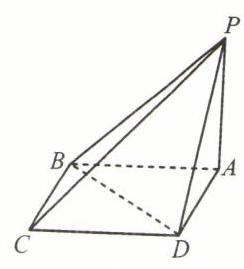
\includegraphics[width=0.2\textwidth]{bodyxb/src/bo_d20aucref24c73anc48g_187_1193_915_244_269_0.jpg}
\end{center}


(第 51 题)

(1)平面 ${PBD}$ 与底面 ${ABCD}$ 所成锐二面角的大小；

(2)点 $A$ 到平面 ${PBD}$ 的距离.

52. (1) 已知棱锥的底面积为 ${150}{\mathrm{{cm}}}^{2}$ ,平行于底的截面面积为 ${54}{\mathrm{{cm}}}^{2}$ ,底面和截面的距离为 ${14}\mathrm{{cm}}$ ,求该棱锥的高；

(2)已知正六棱锥 $S - {ABCDEF}$ 的侧棱 ${SA} = {10}\mathrm{{cm}}$ ,底面边长为 $8\mathrm{{cm}}$ ,该正棱锥被平行于底面的平面所截,截面面积为 $\dfrac{32}{3}\sqrt{3}{\mathrm{{cm}}}^{2}$ ,求截面和底面之间的距离.

\section*{(B)}

53. 若一个三棱锥的底面是直角三角形, 则它的三个侧面 (   )

(A) 一定都不是直角三角形. (B) 至多有一个是直角三角形.

(C)至多有两个是直角三角形. (D) 三个都可以是直角三角形.

54. 在四棱锥的四个侧面中,直角三角形的最多个数是(   )

(A) 4 . (B) 3. (C) 2. (D) 1 .

55. 若正四棱锥的全面积是它底面面积的 3 倍, 则侧面与底面所成二面角的余弦值为 (   )

(A) $\dfrac{\sqrt{3}}{2}$ . (B) $\dfrac{1}{2}$ . (C) $\dfrac{1}{3}$ . (D) $\dfrac{1}{6}$ .

56. 若正四面体 ${PEFH}$ 中, $M,N$ 分别为 ${PH},{EF}$ 的中点,则异面直线 ${MN}$ 与 ${PE}$ 所成的角等于(   )

(A) ${90}^{ \circ  }$ . (B) ${60}^{ \circ  }$ . (C) ${45}^{ \circ  }$ . (D) ${30}^{ \circ  }$ .

57. 一个棱锥被平行于底面的平面所截,若截面面积与底面面积之比为 $1 : 2$ ,则此棱锥的一条侧棱被截面所分成的两段线段(自上而下)之比是(   )

(A) $1 : 4$ . (B) $1 : \sqrt{2}$ . (C) $1 : \left( {\sqrt{2} + 1}\right)$ . (D) $1 : \left( {\sqrt{2} - 1}\right)$ .

58. 已知一棱锥被平行于底面的平面所截,且截面与底面的面积之比为 $1 : \sqrt{2}$ ,则此棱锥的高被截面所分成的两段线段 (自上而下) 之比是 (   )

(A) $1 : 2$ . (B) $1 : \sqrt{2}$ . (C) $1 : \left( {\sqrt[3]{2} - 1}\right)$ . (D) $1 : \left( {\sqrt[4]{2} - 1}\right)$ .

59. 两个平行于底面的截面将棱锥的侧面积分成三个相等的部分, 则这两个截面将棱锥的高分成的三段线段(自上而下)之比是(   )

(A) $1 : \sqrt{2} : \sqrt{3}$ . (B) $1 : \left( {\sqrt{2} - 1}\right)  : \left( {\sqrt{3} - 1}\right)$ .

(C) $1 : \left( {\sqrt{2} - 1}\right)  : \left( {\sqrt{3} - \sqrt{2}}\right)$ . (D) $1 : \left( {\sqrt{2} + 1}\right)  : \left( {\sqrt{3} + \sqrt{2}}\right)$ .

60. 若四棱锥的四个侧面与底面所成的角都相等,则其底面四边形必是(   )

(A) 矩形. (B) 菱形.

(C) 圆外切四边形. (D) 圆内接四边形.

61. 如果一个棱锥的各棱都相等,那么这个棱锥必定不是(   )

(A) 三棱锥. (B) 四棱锥.

(C) 五棱锥. (D) 正六棱锥.

62. 底面边长为 $a$ ,高为 $h$ 的正六棱锥的侧面积等于(   )

(A) $\dfrac{a}{4}\sqrt{4{h}^{2} + 3{a}^{2}}$ . (B) $\dfrac{3a}{2}\sqrt{4{h}^{2} + 3{a}^{2}}$ .

(C) $\dfrac{3a}{2}\sqrt{4{h}^{2} - 3{a}^{2}}$ . (D) ${3a}\sqrt{{h}^{2} + {a}^{2}}$ .

63. 三棱锥的三条侧棱两两互相垂直,三个侧面与底面所成的二面角都相等,则顶点在底面三角形上的射影是底面三角形的(   )

(A) 垂心但非内心. (B) 内心但非外心.

(C) 外心、垂心但非内心. (D) 中心.

64. 正四棱锥相邻两侧面所成的二面角(   )

(A) 一定是锐角.

(B) 一定是钝角.

(C) 有可能是直角.

(D) 可能是锐角, 也可能是钝角, 但不可能是直角.

65. 在正六棱锥 $P - {ABCDEF}$ 中,已知 ${O}_{1}$ 是 $\bigtriangleup {BPE}$ 的外心, ${O}_{2}$ 是 $\bigtriangleup {APB}$ 的外心,则 ${O}_{1}{O}_{2}$ 和侧面 ${APB}$ 所成的角为(   )

(A) ${30}^{ \circ  }$ . (B) ${45}^{ \circ  }$ . (C) ${60}^{ \circ  }$ . (D) ${90}^{ \circ  }$ .

66. 若一个三棱锥的三个侧面都是等腰三角形,则此三棱锥一定是(   )

(A) 正三棱锥. (B) 至少有两个侧面的面积相等.

(C) 底面不可能是直角三角形. (D) 底面可以是任意三角形.

67. 过四面体同一顶点的三条棱的中点可以确定一个截面, 这样的截面共有四个. 用这四个截面截去四个小棱锥后剩下的几何体的表面积与原四面体的表面积之比等于(   )

(A) $1 : 4$ . (B) $1 : 3$ . (C) $1 : 2$ . (D) $2 : 3$ .

68. (1)在侧棱和底面边长都相等的正三棱锥 $A - {BCD}$ 中, $E$ 为侧棱 ${AD}$ 的中点,则:

① ${CE}$ 和底面 ${BCD}$ 所成角的正弦值为\blkda{},

② ${CE}$ 和 ${AB}$ 所成角的余弦值为\blkda{}；

(2)在正三棱锥 $P - {ABC}$ 中,已知底面边长 ${AB} = 1$ ,侧棱 ${PA} = \sqrt{2},D,E$ 分别为 ${AB},{PC}$ 的中点, 则:

① 异面直线 ${PD}$ 与 ${BE}$ 所成角的余弦值为\blkda{},

② ${BE}$ 与平面 ${ABC}$ 所成角的正弦值为\blkda{}；

(3)已知三棱锥 $A - {BCD}$ 的高 ${AH} = 3\sqrt{3}a$ ,且 $H$ 为底面 $\bigtriangleup  {BCD}$ 的重心,若 ${AB} = {AC}$ ,二面角 $A - {BC} - D$ 等于 ${60}^{ \circ  },G$ 为 $\bigtriangleup  {ABC}$ 的重心,则 ${HG}$ 的长等于\blkda{}.

69. 在正四棱锥 $P - {ABCD}$ 中,

(1)已知侧棱长与底面边长相等, $E$ 是 ${PA}$ 的中点(如图),则异面直线 ${BE}$ 与 ${PC}$ 所成角的余弦值是\blkda{}；

\begin{center}
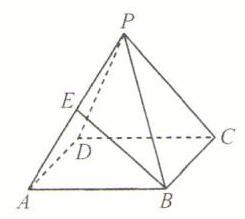
\includegraphics[width=0.2\textwidth]{bodyxb/src/bo_d20aucref24c73anc48g_189_469_1010_245_219_0.jpg}
\end{center}


[第 69(1)题]

\begin{center}
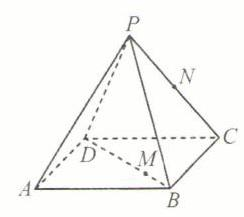
\includegraphics[width=0.2\textwidth]{bodyxb/src/bo_d20aucref24c73anc48g_189_919_1007_244_217_0.jpg}
\end{center}


[第 69(2)题]

(2)已知高为 2,底面边长为 $\sqrt{2}$ ,点 $M$ , $N$ 分别在线段 ${BD}$ 与 ${PC}$ 上(如图),则 $M$ , $N$ 两点间的最短距离为\blkda{}.

70. 在正三棱锥 $P - {ABC}$ 中,已知底面边长为 12,高 ${PO}$ 为 $8,M$ 为 ${PA}$ 上一点,求截面 $\bigtriangleup {MBC}$ 面积的最小值.

71. 已知三棱锥 $P - {ABC}$ 的底面 $\bigtriangleup  {ABC}$ 内接于 $\odot  O$ ,其中 ${AB}$ 为 $\odot  O$ 的直径, $\cos \angle {ABC} = \dfrac{5}{6}$ ,又 ${PA} \bot$ 平面 ${ABC}$ ,且 ${PA} : {AB} = 4 : 3$ (如图),求直线 ${PB}$ 和平面 ${PAC}$ 所成角的大小.

\begin{center}
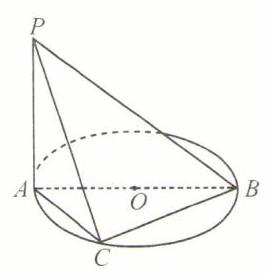
\includegraphics[width=0.2\textwidth]{bodyxb/src/bo_d20aucref24c73anc48g_189_283_1683_268_276_0.jpg}
\end{center}


(第 71 题)

\begin{center}
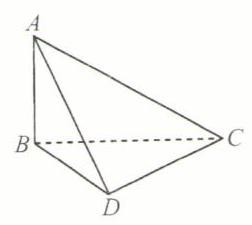
\includegraphics[width=0.2\textwidth]{bodyxb/src/bo_d20aucref24c73anc48g_189_675_1730_252_225_0.jpg}
\end{center}


(第 72 题)

\begin{center}
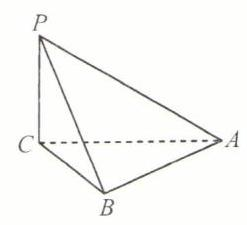
\includegraphics[width=0.2\textwidth]{bodyxb/src/bo_d20aucref24c73anc48g_189_1049_1726_247_225_0.jpg}
\end{center}


(第 73 题)

72. 在三棱锥 $A - {BCD}$ 中,已知 ${AB} \bot$ 平面 ${BCD},{BD} \bot  {CD}$ (如图).

(1)求证:平面 ${ABD} \bot$ 平面 ${ACD}$ ；

(2)若 ${AB} = {BC} = {2BD}$ ,求二面角 $B - {AC} - D$ 的正弦值.

73. 在三棱锥 $P - {ABC}$ 中,已知棱 ${PC},{AC},{BC}$ 两两互相垂直,且 $\angle {PAC} = {30}^{ \circ  },{PB} = \sqrt{13},{BC}$  $= 3$ (如图).

(1)求二面角 $B - {PA} - C$ 的度数；

(2)设点 $C$ 在面 ${PAB}$ 上的射影为 $O$ ,求点 $O$ 到平面 ${PAC}$ 的距离.

74. 在三棱锥 $P - {ABC}$ 中,已知 ${PA} = {PB},{CB}\bot$ 面 ${PAB},M$ 为 ${PC}$ 的中点, $N$ 在棱 ${AB}$ 上,且 ${AN} = {3NB}$ (如图).

(1)求证: ${MN}\bot {AB}$ ；

(2)当 $\angle {APB} = {90}^{ \circ  },{BC} = 2,{AB} = 4$ 时,求 ${MN}$ 的长.

\begin{center}
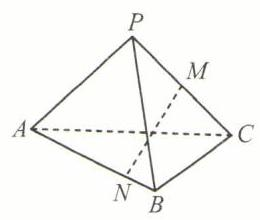
\includegraphics[width=0.2\textwidth]{bodyxb/src/bo_d20aucref24c73anc48g_190_413_629_260_220_0.jpg}
\end{center}


(第 74 题)

\begin{center}
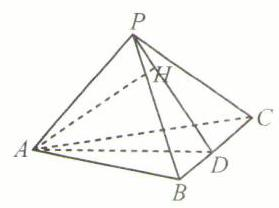
\includegraphics[width=0.2\textwidth]{bodyxb/src/bo_d20aucref24c73anc48g_190_934_638_279_208_0.jpg}
\end{center}


(第 75 题)

75. 在正三棱锥 $P - {ABC}$ 中,已知 $A$ 在侧面 ${PBC}$ 上的射影为点 $H$ ,连接 ${PH}$ 并延长交 ${BC}$ 于点 $D$ ,且 $\dfrac{PH}{PD} = \dfrac{1}{4}$ (如图),求侧面与底面所成二面角的大小.

76. 在三棱锥 $P - {ABC}$ 中 (如图),

(1)已知侧棱 ${PA},{PB},{PC}$ 两两互相垂直,且 ${PA} = {PB} = 1,{PC} = 2$ ,求: ①点 $P$ 到底面 ${ABC}$ 的距离, ②二面角 $P - {BC} - A$ 的正弦值； ( 2 )已知侧棱与底面都成 ${75}^{ \circ  }$ 的角,且 $\bigtriangleup  {ABC}$ 的三内角 $\angle {BAC} : \angle {ABC} : \angle {ACB} = 1 : 2$  $: 9,{AC} = 3$ ,求此棱锥的高;

(3)已知侧面与底面都成 ${45}^{ \circ  }$ 角, $\angle {ABC} = {60}^{ \circ  }$ ,两边 ${AB}$ , ${BC}$ 的长是方程 $3{x}^{2} - {27x} + {32} =$ 0 的两根, 求此棱锥的高.

\begin{center}
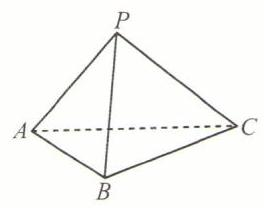
\includegraphics[width=0.2\textwidth]{bodyxb/src/bo_d20aucref24c73anc48g_190_307_1563_264_208_0.jpg}
\end{center}


(第 76 题)

\begin{center}
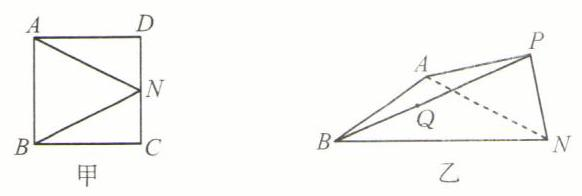
\includegraphics[width=0.4\textwidth]{bodyxb/src/bo_d20aucref24c73anc48g_190_764_1570_582_196_0.jpg}
\end{center}


(第 77 题)

77. 已知 $N$ 是边长为 2 的正方形 ${ABCD}$ 的边 ${CD}$ 的中点 (如图甲),沿 ${AN},{BN}$ 折起,使 $C,D$ 两点重合于一点 $P$ (如图乙),在三棱锥 $P - {ABN}$ 的棱 ${PB}$ 上取一点 $Q$ ,过点 $Q$ 作平行于 ${PN},{AB}$ 的截面,若要使截面面积最大,点 $Q$ 应取在何处? 其截面面积的最大值是多少?

78. 已知 $\bigtriangleup {BCD}$ 内接于直角梯形 ${A}_{1}{A}_{2}{A}_{3}D$ (如图甲),沿 $\bigtriangleup {BCD}$ 的三边分别将 $\bigtriangleup {A}_{1}{BD}$ , $\bigtriangleup {A}_{2}{BC},\bigtriangleup {A}_{3}{CD}$ 翻折上去,恰好形成一个三棱锥 $A - {BCD}\left( {{A}_{1},{A}_{2},{A}_{3}}\right.$ 重合于一点 $\left. A\right)$ .

(1)在三棱锥中,求证: ${AB}\bot {CD}$ ；

(2)若直角梯形上底 ${A}_{1}D = {10}$ ,高 ${A}_{1}{A}_{2} = 8$ ,求翻折后三棱锥的侧面 ${ACD}$ 和底面 ${BCD}$ 所成二面角的正切值.

\begin{center}
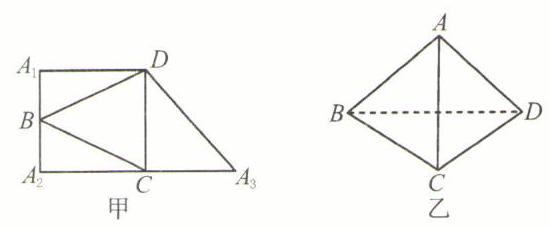
\includegraphics[width=0.4\textwidth]{bodyxb/src/bo_d20aucref24c73anc48g_191_228_274_550_228_0.jpg}
\end{center}


(第 78 题)

\begin{center}
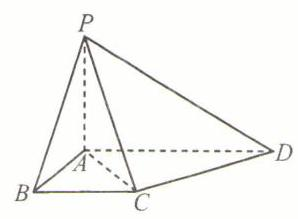
\includegraphics[width=0.2\textwidth]{bodyxb/src/bo_d20aucref24c73anc48g_191_938_282_298_219_0.jpg}
\end{center}


(第 79 题)

79. 在四棱锥 $P - {ABCD}$ 中,已知 $\angle {DAB} = \angle {ABC} = {90}^{ \circ  },{PA}\bot$ 平面 ${ABCD},{AB} = {BC} = 1$ , ${AD} = 2$ (如图),求证: ${CD} \bot$ 平面 ${PAC}$ .

80. 求证:若三棱锥的顶点到底面的射影是底面三角形的垂心,则底面三角形的任一顶点到所对侧面的射影也必是此侧面三角形的垂心.

81. 已知正三棱锥的底面边长为 2,高为 $\dfrac{\sqrt{6}}{6}$ ,求其两侧面所成二面角的大小.

82. 已知正四棱锥侧棱与底面成 $\alpha$ 角,侧面与底面成 $\beta$ 角,相邻两侧面成 $\gamma$ 角,求证:

(1) $\cot \alpha  \cdot  \tan \beta  = \sqrt{2}$ ；

(2) $\sin \alpha  \cdot  \tan \dfrac{\gamma }{2} = 1$ ；

(3) $\cos \gamma  + {\cos }^{2}\beta  = 0$ .

\begin{center}
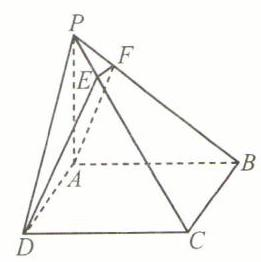
\includegraphics[width=0.2\textwidth]{bodyxb/src/bo_d20aucref24c73anc48g_191_1179_1125_261_262_0.jpg}
\end{center}


(第 83 题)

83. 在四棱锥 $P - {ABCD}$ 中,已知 ${PA}\bot$ 底面 ${ABCD},{PA} = 3,\angle {PDC} =$  ${90}^{ \circ  }$ ,底面 ${ABCD}$ 各边长都等于 4,过 ${AD}$ 作与 ${PB}$ 垂直的截面交 ${PB}$ 于点 $F$ ,交 ${PC}$ 于点 $E$ (如图).

(1)求证: ${EF} \bot$ 平面 ${PAB}$ ；

(2)求截面 ${ADEF}$ 的面积；

(3)求二面角 $F - {AD} - B$ 的余弦值.

\section*{二、旋转体}

\section*{(一) 圆柱}

\section*{【典型题型和解题技巧】}

1. 圆柱的截面.

圆柱的截面有四种:

(1)横截面. 即与底面平行的截面 (如图 12), 显然, 横截面与底面全等.

(2)轴截面. 即过圆柱轴的截面 (如图 13),显然,轴截面是一个矩形. 轴截面为正方形的圆柱称为等边圆柱.

(3)纵截面. 即与圆柱的轴平行的截面 (如图 14),是一个矩形,轴与纵截面的距离就是底面圆心到纵截面一边的距离 (即弦心距).

(4)斜截面. 即与圆柱的轴斜交的截面 (如图 15). 证明斜截面是一个椭圆面在高中课本中不作要求.

\begin{center}
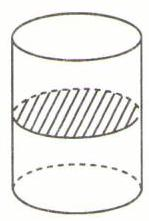
\includegraphics[width=0.2\textwidth]{bodyxb/src/bo_d20aucref24c73anc48g_192_329_374_149_221_0.jpg}
\end{center}


(图 12)

\begin{center}
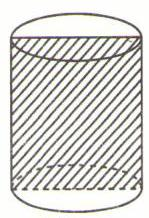
\includegraphics[width=0.2\textwidth]{bodyxb/src/bo_d20aucref24c73anc48g_192_608_374_149_218_0.jpg}
\end{center}


(图 13)

\begin{center}
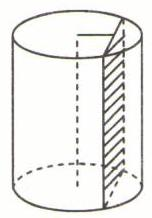
\includegraphics[width=0.2\textwidth]{bodyxb/src/bo_d20aucref24c73anc48g_192_886_373_152_218_0.jpg}
\end{center}


(图 14)

\begin{center}
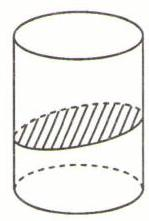
\includegraphics[width=0.2\textwidth]{bodyxb/src/bo_d20aucref24c73anc48g_192_1163_369_149_221_0.jpg}
\end{center}


(图 15)

例 1 已知圆柱的轴为 $O{O}_{1},A,B$ 分别为上、下底面圆周上的点, $O{O}_{1} = 4,{OA} = 3$ ,且 ${OA}$ 与 ${O}_{1}B$ 成 ${60}^{ \circ  }$ 角. 求:

(1) $O{O}_{1}$ 与 ${AB}$ 所成角的正切值；

\begin{center}
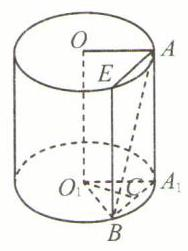
\includegraphics[width=0.2\textwidth]{bodyxb/src/bo_d20aucref24c73anc48g_192_1290_796_188_251_0.jpg}
\end{center}


(图 16)

(2)过 ${AB}$ 且与 $O{O}_{1}$ 平行的平面和 $O{O}_{1}$ 的距离；

(3)过 ${AB}$ 且与 $O{O}_{1}$ 平行的截面的面积；

(4)异面直线 $O{O}_{1}$ 与 ${AB}$ 的距离.

解 (1) 如图 16,设过 $A$ 的母线为 $A{A}_{1}$ ,连接 ${O}_{1}{A}_{1}$ ,则由 $A{A}_{1}//O{O}_{1}$ ,知 $\angle {BA}{A}_{1}$ 就是 $O{O}_{1}$ 与 ${AB}$ 所成的角或其补角,

$\because {O}_{1}{A}_{1}//{OA},\therefore \angle {A}_{1}{O}_{1}B$ (或其补角) 就是 ${OA}$ 与 ${O}_{1}B$ 所成的角.

由条件得 $\angle {A}_{1}{O}_{1}B = {60}^{ \circ  }$ 或 ${120}^{ \circ  },{A}_{1}B = 3$ 或 $3\sqrt{3}$ . 又 $A{A}_{1} = O{O}_{1} = 4$ ,

$\therefore \tan \angle {BA}{A}_{1} = \dfrac{{A}_{1}B}{A{A}_{1}} = \dfrac{3}{4}$ 或 $\dfrac{3\sqrt{3}}{4}$ .

(2)由 ${O}_{1}O//A{A}_{1}$ ,得 $O{O}_{1}//$ 平面 $A{A}_{1}B$ . 取 ${A}_{1}B$ 的中点 $C$ ,连接 ${O}_{1}C$ ,则 ${O}_{1}C \bot  {A}_{1}B$ .

又 $\because {O}_{1}C \bot  A{A}_{1},\therefore {O}_{1}C \bot$ 平面 $A{A}_{1}B$ ,故 ${O}_{1}C$ 就是 $O{O}_{1}$ 与平面 $A{A}_{1}B$ 间的距离. 容易算得 ${O}_{1}C = \dfrac{3\sqrt{3}}{2}$ 或 $\dfrac{3}{2}$ .

(3)显然,过 ${AB}$ 且与 $O{O}_{1}$ 平行的截面就是矩形 $A{A}_{1}{BE}(E$ 为过 $B$ 的母线与上底面的交点),其面积 $S = A{A}_{1} \cdot  {A}_{1}B = {12}$ 或 ${12}\sqrt{3}$ .

(4)由第(2)题知 ${O}_{1}O//$ 平面 $A{A}_{1}B$ ,故 ${O}_{1}O$ 与平面 $A{A}_{1}B$ 的距离就是 $O{O}_{1}$ 与 ${AB}$ 间的距离,故所求的距离为 $\dfrac{3\sqrt{3}}{2}$ 或 $\dfrac{3}{2}$ .

注意 本例也可直接作出 $O{O}_{1}$ 与 ${AB}$ 的公垂线段来求 $O{O}_{1}$ 与 ${AB}$ 的距离,请读者试一试.

2. "短程线" 与 "展".

“展”是立体几何中的一种解题方法, 在圆柱这一单元中, “展”主要是用来求 “短程线”.

例 2 已知 ${AB}{B}_{1}{A}_{1}$ 是圆柱的轴截面, $A{A}_{1} = a,{AB} = \dfrac{3}{4}a,P$ 是 $B{B}_{1}$ 的中点. 沿圆柱的侧面从 ${A}_{1}$ 拉一根绳子到 $P$ ,求绳子的最短长度.

解 如图 17,将圆柱的侧面展开,则 ${A}_{1}C = \dfrac{3}{8}{\pi a}$ . 而 ${CP} = \dfrac{a}{2}$ ,故绳子的最短长度为 $\sqrt{\dfrac{9{\pi }^{2}{a}^{2}}{64} + \dfrac{{a}^{2}}{4}} = \dfrac{a}{8}\sqrt{9{\pi }^{2} + {16}}$ .

\begin{center}
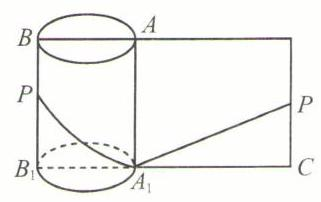
\includegraphics[width=0.2\textwidth]{bodyxb/src/bo_d20aucref24c73anc48g_193_1114_139_321_202_0.jpg}
\end{center}


(图 17)

\section*{【训练题】}

\section*{(A)}

84. 若圆柱的轴截面面积为 $S$ ,则圆柱的侧面积为 (   )

(A) ${4\pi S}$ . (B) ${2\pi S}$ . (C) ${\pi S}$ . (D) $\dfrac{1}{2}{\pi S}$ .

85. 先作一个圆柱的内接正三棱柱,再作这个正三棱柱的内切圆柱,则这两个圆柱的侧面积之比是(   )

(A) $1 : \sqrt{3}$ . (B) $1 : 2$ . (C) $1 : 3$ . (D) $1 : 4$ .

86. 已知圆柱的侧面展开图是一个矩形 ${ABCD}$ ,其中 ${AD}$ 是一条母线,且矩形的对角线 ${AC} = 8$  $\mathrm{{cm}},\angle {BAC} = {30}^{ \circ  }$ ,则圆柱的侧面积是(   )

(A) $4\sqrt{3}{\mathrm{{cm}}}^{2}$ . (B) $8\sqrt{3}{\mathrm{{cm}}}^{2}$ . (C) ${16}\sqrt{3}{\mathrm{{cm}}}^{2}$ . (D) ${32}\sqrt{3}{\mathrm{{cm}}}^{2}$ .

87. 已知圆柱的底面半径是 ${20}\mathrm{{cm}}$ ,高为 ${15}\mathrm{{cm}}$ ,则平行于圆柱的轴且与此轴相距 ${12}\mathrm{{cm}}$ 的截面面积是(   )

(A) ${480}{\mathrm{{cm}}}^{2}$ . (B) ${450}{\mathrm{{cm}}}^{2}$ . (C) ${320}{\mathrm{{cm}}}^{2}$ . (D) ${240}{\mathrm{{cm}}}^{2}$ .

88. 若圆柱的高增大到原来的 3 倍, 底面直径增大到原来的 4 倍, 则此圆柱的侧面积增大到原来的(   )

(A) 24 倍. (B) 16 倍. (C) 12 倍. (D) 9 倍.

89. (1)圆柱的轴截面是 $S$ ,则它的侧面积是\blkda{}；

(2)一个圆柱的轴截面是面积为 $Q$ 的正方形,那么圆柱的表面积是\blkda{}；

(3)圆柱的侧面展开图的对角线长为 $8\mathrm{{cm}}$ ,对角线与侧面展开图矩形的一边成 ${30}^{ \circ  }$ 角,则圆柱的全面积为\blkda{}.

90. (1) 以正方形的一边所在直线为轴旋转一周得到一个圆柱, 则圆柱的全面积与轴截面面积的比值为\blkda{}；

(2)已知一个圆柱的底面积为 ${4\pi }$ ,其侧面展开图是正方形,则它的侧面积为\blkda{}.

91. 圆柱的一个截面 ${A}_{1}{AB}{B}_{1}//$ 轴 ${O}_{1}O$ (如图).

\begin{center}
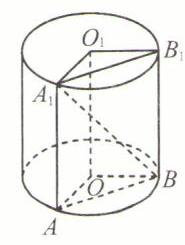
\includegraphics[width=0.2\textwidth]{bodyxb/src/bo_d20aucref24c73anc48g_193_1248_1821_185_245_0.jpg}
\end{center}


(第 91 题)

(1)若 ${O}_{1}{A}_{1} = {13}$ ,截面与 ${O}_{1}O$ 距离为 5,且截面面积为 48,则 ${A}_{1}A$ =\blkda{}；

(2)若截面把圆柱侧面面积分成 $1 : 3$ 的两部分,则 ${O}_{1}O$ 与截面的距离是 ${O}_{1}{A}_{1}$ 的\blkda{}倍；

(3)若 ${O}_{1}{A}_{1}$ 和 ${OB}$ 成 $\theta$ 角,且 ${O}_{1}{A}_{1} = R,{A}_{1}A = h$ ,则 ${O}_{1}O$ 与 ${A}_{1}B$ 所成角的正切值等于\blkda{}.

92. 已知圆柱的高是 ${12}\mathrm{{cm}}$ ,底面半径为 $6\mathrm{{cm}}$ ,若上、下底面的半径 ${OA}$ , ${O}^{\prime }B$ 互相垂直 (如图),求线段 ${AB}$ 的长.

\begin{center}
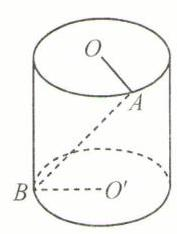
\includegraphics[width=0.2\textwidth]{bodyxb/src/bo_d20aucref24c73anc48g_194_1303_191_177_234_0.jpg}
\end{center}


(第 92 题)

93. 圆柱的母线长为 ${10}\mathrm{{cm}}$ ,用一平行于轴且与轴相距 $2\mathrm{{cm}}$ 的平面去截这个圆柱,且截面在圆柱底面截得的劣弧所对的圆心角为 ${120}^{ \circ  }$ ,求此截面的面积.

\section*{(B)}

94. 已知圆柱轴截面的对角线为定值, 要使圆柱的侧面积最大, 轴截面对角线与底面所成的角应为(   )

(A) $\dfrac{\pi }{3}$ . (B) $\dfrac{\pi }{4}$ . (C) $\dfrac{\pi }{9}$ . (D) $\dfrac{\pi }{8}$ .

95. 已知圆柱的侧面积为 ${4\pi }$ ,则当轴截面的对角线长取最小值时,圆柱母线长 $l$ 与底面半径 $r$ 的关系是(   )

(A) $l = r$ . (B) $l = {2r}$ .

(C) $l = {3r}$ . (D) $l = {4r}$ .

96. 已知圆柱的轴截面 ${ABCD}$ 是边长为 $5\mathrm{{cm}}$ 的正方形,则从下底面的点 $A$ 到上底面的点 $C$ 绕圆柱侧面的最短距离是(   )

(A) ${10}\mathrm{{cm}}$ . (B) $5\sqrt{2}\mathrm{{cm}}$ .

(C) $5\sqrt{{\pi }^{2} + 1}\mathrm{{cm}}$ . (D) $\dfrac{5}{2}\sqrt{{\pi }^{2} + 4}\mathrm{{cm}}$ .

97. 已知 $A,B$ 分别是圆柱的上、下底面圆周上的点, $O,{O}_{1}$ 分别是上、下底面的圆心 (如图).

(1)若 ${OA} = 3,{O{O}_{1}} = 4,{AB} = 5$ ,求 ${AB}$ 和 $O{O}_{1}$ 的距离；

(2)若此圆柱是等边圆柱(即高与底面图的直径相等),且高为 ${2a}$ , ${AB}$ 与底面成 $\alpha$ 角,求

${AB}$ 和 $O{O}_{1}$ 的距离;

(3)若 ${OA} = R,{O{O}_{1}} = h,{OA}$ 与 ${O}_{1}B$ 成 $\alpha$ 角,求柱面上 $A,B$ 的最短距离.

\begin{center}
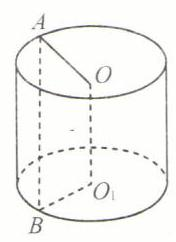
\includegraphics[width=0.2\textwidth]{bodyxb/src/bo_d20aucref24c73anc48g_194_507_1596_176_242_0.jpg}
\end{center}


(第 97 题)

\begin{center}
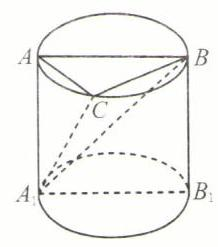
\includegraphics[width=0.2\textwidth]{bodyxb/src/bo_d20aucref24c73anc48g_194_979_1585_218_247_0.jpg}
\end{center}


(第 98 题)

98. 已知圆柱的轴截面为 $A{A}_{1}{B}_{1}B,C$ 是上底面圆周上一点 (如图),求证:

(1)截面 $A{A}_{1}C \bot$ 截面 $B{A}_{1}C$ ；

(2)若二面角 $A - {A}_{1}B - C$ 为 $\alpha ,\angle {CAB} = \beta ,\angle C{A}_{1}B = \gamma$ ,则 $\sin a = \dfrac{\cos \beta }{\cos \gamma }$ .

99. 正方形 ${AB}{B}_{1}{A}_{1}$ 的边长为 ${15}\mathrm{{cm}}$ ,其内有两点 $P,Q$ ,点 $P$ 到 ${A}_{1}A,{A}_{1}{B}_{1}$ 的距离均为 $3\mathrm{{cm}}$ ,

$Q$ 到边 ${AB},B{B}_{1}$ 的距离分别为 $2\mathrm{{cm}}$ 和 $4\mathrm{{cm}}$ (如图甲). 现将正方形卷成一个圆柱,使 ${AB}$ 和 ${A}_{1}{B}_{1}$ 重合 (如图乙),求此时 $P,Q$ 两点间的距离.

\begin{center}
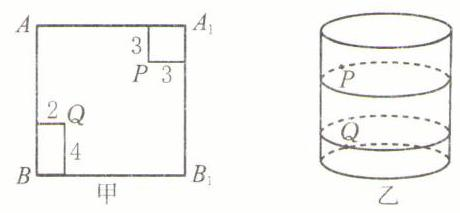
\includegraphics[width=0.3\textwidth]{bodyxb/src/bo_d20aucref24c73anc48g_195_283_290_460_213_0.jpg}
\end{center}


(第 99 题)

\begin{center}
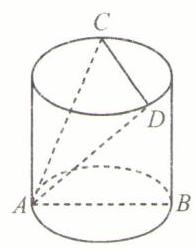
\includegraphics[width=0.2\textwidth]{bodyxb/src/bo_d20aucref24c73anc48g_195_1033_251_196_250_0.jpg}
\end{center}


(第 100 题)

100. 一个圆柱的底面半径为 $R$ ,上底一条弦 ${CD}$ 长为 $a\left( {R < a < {2R}}\right)$ ,它与下底一条直径 ${AB}$ 成 ${60}^{ \circ  }$ 角,平面 ${ACD}$ 与下底面成 ${45}^{ \circ  }$ 角 (如图). 求圆柱的高.

\section*{(二) 圆锥}

\section*{【典型题型和解题技巧】}

1. 圆锥侧面展开图.

有关圆锥的不少问题与它的侧面展开图有关, 在画图的时候, 应将圆锥及其侧面的展开图作在一幅图中 (如图 18),有助于了解各元素之间的关系.

\begin{center}
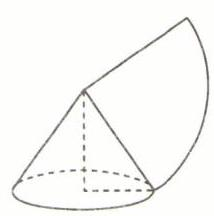
\includegraphics[width=0.2\textwidth]{bodyxb/src/bo_d20aucref24c73anc48g_195_1204_983_214_216_0.jpg}
\end{center}


(图 18)

例 1 一圆台的上、下底面半径分别为 $5\mathrm{{cm}}$ 和 ${10}\mathrm{{cm}}$ ,母线 ${AB}$ 长 ${20}\mathrm{{cm}}$ , 从 ${AB}$ 的中点 $M$ 拉一根绳子,绕圆台侧面到达点 $B$ ,试求绳长的最小值.

分析 在圆台侧面上,绳长很难计算,若将圆台侧面沿母线 ${AB}$ 展开,可以得到平面上的一个部分圆环, 问题就转化为求平面上的线段长.

解 如图 19,设圆台由圆锥截得,将圆锥沿母线 ${OB}$ 展开,得一扇形 ${OB}{B}^{\prime }$ ,则 $M{B}^{\prime }$ 即为所求.

\begin{center}
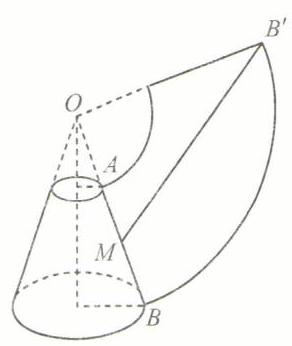
\includegraphics[width=0.2\textwidth]{bodyxb/src/bo_d20aucref24c73anc48g_195_1124_1323_292_346_0.jpg}
\end{center}


(图 19)

$\angle {BO}{B}^{\prime } = \dfrac{{10} - 5}{20} \cdot  {360}^{ \circ  } = {90}^{ \circ  },$

$\because \dfrac{OA}{{OA} + {20}} = \dfrac{5}{10},\therefore {OA} = {20}$ .

$\therefore {OM} = {30}$ ,而 $O{B}^{\prime } = {40}$ ,

$\therefore M{B}^{\prime } = \sqrt{O{M}^{2} + O{B}^{\prime 2}} = {50}\mathrm{{cm}}$ ,

即所求绳长的最小值为 ${50}\mathrm{{cm}}$ . 2. 过顶点且面积最大的截面.

圆锥过顶点的截面是一个等腰三角形 (如图 20), 当这个截面同时过圆锥的轴时, 就成了轴截面 (如图 21).

\begin{center}
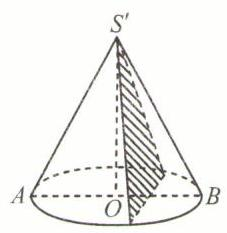
\includegraphics[width=0.2\textwidth]{bodyxb/src/bo_d20aucref24c73anc48g_196_350_143_227_233_0.jpg}
\end{center}


(图 20)

\begin{center}
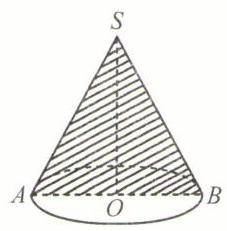
\includegraphics[width=0.2\textwidth]{bodyxb/src/bo_d20aucref24c73anc48g_196_707_143_227_231_0.jpg}
\end{center}


(图 21)

\begin{center}
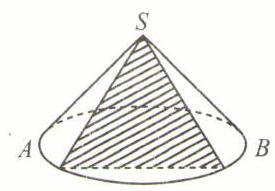
\includegraphics[width=0.2\textwidth]{bodyxb/src/bo_d20aucref24c73anc48g_196_1058_182_275_191_0.jpg}
\end{center}


(图 22)

需要特别强调的是,圆锥过顶点且面积最大的截面并不一定是轴截面. 假设圆锥的母线是 $l$ ,轴截面的顶角为 $\alpha$ ,那么:

当 $\alpha  \leq  {90}^{ \circ  }$ 时,面积最大的截面就是轴截面,它的面积为 $\dfrac{1}{2}{l}^{2}\sin \alpha$ ;

当 $\alpha  > {90}^{ \circ  }$ 时,面积最大的截面不是轴截面,而是过圆锥顶点且顶角是 ${90}^{ \circ  }$ 的截面(如图 22), 它的面积是 $\dfrac{1}{2}{l}^{2}$ .

例 2 将半径为 $l$ ,圆心角为 ${240}^{ \circ  }$ 的扇形卷成一个圆锥的侧面,求过顶点的截面面积的最大值.

解 如图 23,设圆锥的底面半径为 $r$ ,轴截面顶角为 $\alpha$ ,

\begin{center}
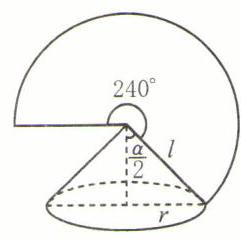
\includegraphics[width=0.2\textwidth]{bodyxb/src/bo_d20aucref24c73anc48g_196_1251_888_241_239_0.jpg}
\end{center}


(图 23)

则由 ${240}^{ \circ  } = \dfrac{r}{l}{360}^{ \circ  }$ ,得 $\dfrac{r}{l} = \dfrac{2}{3}$ .

于是 $\sin \dfrac{\alpha }{2} = \dfrac{r}{l} = \dfrac{2}{3} < \dfrac{\sqrt{2}}{2}$ ,从而得 $\alpha  < {90}^{ \circ  }$ .

$\therefore$ 过顶点且面积最大的截面就是圆锥的轴截面,它的面积为

$\dfrac{1}{2}{l}^{2}\sin \alpha  = {l}^{2} \cdot  \sin \dfrac{\alpha }{2}\cos \dfrac{\alpha }{2} = {l}^{2} \cdot  \dfrac{2}{3} \cdot  \dfrac{\sqrt{5}}{3} = \dfrac{2\sqrt{5}}{9}{l}^{2}.$

\section*{【训练题】}

\section*{(A)}

101. 轴截面为等边三角形的圆锥(即等边圆锥)的侧面积与全面积之比为(   )

(A) $2 : 3$ . (B) $4 : 5$ . (C) $\sqrt{3} : 2$ . (D) $1 : 2$ .

102. 已知圆锥的侧面积与全面积之比为 $2 : 3$ ,则圆锥轴截面的顶角为(   )

(A) ${30}^{ \circ  }$ . (B) ${45}^{ \circ  }$ . (C) ${60}^{ \circ  }$ . (D) ${90}^{ \circ  }$ .

103. 圆心角为 $\dfrac{3\pi }{4}$ 、面积为 ${S}_{1}$ 的扇形围成一个圆锥的侧面,若此圆锥的全面积为 ${S}_{2}$ ,则 ${S}_{1} : {S}_{2}$ 的值是(   )

(A) $\dfrac{8}{11}$ . (B) $\dfrac{8}{13}$ . (C) $\dfrac{5}{8}$ . (D) $\dfrac{3}{8}$ .

104. 若等边圆锥 (轴截面为等边三角形) 的轴截面面积为 $Q$ ,则此圆锥的侧面积等于(   )

(A) ${3\pi Q}$ . (B) $\dfrac{4}{3}\sqrt{3}{\pi Q}$ . (C) $\dfrac{2}{3}\sqrt{3}{\pi Q}$ . (D) ${\pi Q}$ .

105. 已知圆锥轴截面顶角为锐角,且正弦值为 $\dfrac{24}{25}$ ,则其侧面展开图的圆心角为 (   )

(A) ${108}^{ \circ  }$ . (B) ${144}^{ \circ  }$ . (C) ${180}^{ \circ  }$ . (D) ${216}^{ \circ  }$ .

106. 已知圆锥的高 $h = 8$ ,它的侧面展开图的圆心角是 ${216}^{ \circ  }$ ,则这个圆锥的全面积是(   )

(A) ${96\pi }$ . (B) ${84\pi }$ . (C) ${60\pi }$ . (D) ${24\pi }$ .

107. 已知 ${EF},{MN}$ 是等边圆锥底面互相垂直的两条直径, $P$ 是母线 ${VE}$ 的中点, $O$ 是圆锥底面的中心,记直线 ${PM}$ 与 ${VO}$ 所成的角为 $\theta$ ,则 $\tan \theta$ 的值是 (   )

(A) $\dfrac{\sqrt{6}}{3}$ . (B) $\dfrac{\sqrt{15}}{3}$ . (C) $\dfrac{4\sqrt{6}}{3}$ . (D) $\dfrac{\sqrt{15}}{5}$ .

108. 一个直角梯形,已知上底边长为 $3\mathrm{{cm}}$ ,下底边长为 $7\mathrm{{cm}}$ ,高为 $3\mathrm{{cm}}$ ,以它垂直于底边的腰为轴旋转一周,则所得到的圆台的侧面积是(   )

(A) ${100\pi }{\mathrm{{cm}}}^{2}$ . (B) ${60\pi }{\mathrm{{cm}}}^{2}$ . (C) ${50\pi }{\mathrm{{cm}}}^{2}$ . (D) ${30\pi }{\mathrm{{cm}}}^{2}$ .

109. 已知一个圆台的母线 $l$ 与上、下两底面半径 $r,R$ 满足 ${2l} = r + R$ ,且圆台的侧面积为 ${8\pi }{\mathrm{{cm}}}^{2}$ ,那么母线的长是(   )

(A) $4\mathrm{{cm}}$ . (B) $2\sqrt{2}\mathrm{{cm}}$ . (C) $2\mathrm{{cm}}$ . (D) $\sqrt{2}\mathrm{{cm}}$ .

110. 已知圆台的母线与下底面所成角为 ${60}^{ \circ  }$ ,则它的侧面展开图扇环的圆心角为(   )

(A) ${60}^{ \circ  }$ . (B) ${90}^{ \circ  }$ . (C) ${180}^{ \circ  }$ . (D) ${270}^{ \circ  }$ .

111. 若圆台的两底面半径分别是 1,7 ,则中截面面积是(   )

(A) ${24\pi }$ . (B) ${16\pi }$ . (C) ${8\pi }$ . (D) ${4\pi }$ .

112. 若圆台的上、下底面半径和母线长的比为 $1 : 4 : 5$ ,高为 8 ,则其侧面积为(   )

(A) ${50\pi }$ . (B) ${100\pi }$ . (C) ${150\pi }$ . (D) ${200\pi }$ .

113. (1) 已知圆锥的高是 $\dfrac{32}{3}\mathrm{{cm}}$ ,其侧面展开图的圆心角是 $\dfrac{6}{5}\pi$ 弧度,则其表面积等于\blkda{}cm;

(2)已知 $\bigtriangleup  {ABC}$ 的三边分别是 ${AC} = 3,{BC} = 4,{AB} = 5$ ,以 ${AB}$ 所在直线为轴将此三角形旋转一周,则所得旋转体的表面积等于\blkda{}；

(3)直线 ${MN}$ 与等腰直角三角形 ${ABC}\left( {\angle C = {90}^{ \circ  },{BC} = a}\right)$ 共面,且 ${BC}\bot {MN}$ 于 $B$ ,则 $\bigtriangleup  {ABC}$ 绕 ${MN}$ 旋转一周所得的旋转体的表面积是\blkda{}.

114. (1)如果圆锥的轴截面是等腰直角三角形,则其侧面展开图的扇形圆心角是\blkda{}；

(2)已知一个圆锥侧面展开图是半径为 ${18}\mathrm{{cm}}$ ,圆心角为 ${240}^{ \circ  }$ 的扇形,则这个圆锥底面圆的半径是\blkda{} $\mathrm{{cm}}$ ；

(3)将半径为 $R$ 的圆分割成面积之比为 $1 : 2 : 3$ 的三个扇形作为三个圆锥的侧面,设这三个圆锥的底面半径依次为 ${r}_{1},{r}_{2},{r}_{3}$ ,则 ${r}_{1} + {r}_{2} + {r}_{3}$ 的值是\blkda{}.

115. (1)如果圆锥的底面半径为 $\sqrt{2}$ ,高为 2,则它的侧面积等于\blkda{}；

(2)已知圆锥的侧面积是 ${10}{\mathrm{{cm}}}^{2}$ ,侧面展开图的扇形圆心角是 ${36}^{ \circ  }$ ,则圆锥的全面积是\blkda{} ${\mathrm{{cm}}}^{2}$ ；

(3)若圆锥的侧面积是全面积的 $\dfrac{2}{3}$ ,则圆锥底面直径与高之比为\blkda{}；

(4)如果圆锥的母线和底面所成的角为 $\theta$ ,则圆锥的底面积 ${S}_{\text{ 底 }}$ 与侧面积 ${S}_{\text{ 侧 }}$ 之间的关系是\blkda{}.

116. (1) 过高为 ${10}\mathrm{{cm}}$ 的圆锥顶点作与底面成 ${60}^{ \circ  }$ 角的截面,此截面将圆锥底面周长截成 $1 : 2$ 的两部分,则此截面的面积等于\blkda{} ${\mathrm{{cm}}}^{2}$ ;

(2)已知圆锥的高和母线的夹角为 ${30}^{ \circ  }$ ,在底面圆中有一条长为 $4\mathrm{{cm}}$ 的弦,它所对的圆心角为 ${60}^{ \circ  }$ ,则过圆锥顶点和该弦的截面面积为\blkda{} ${\mathrm{{cm}}}^{2}$ ；

(3)将半径为 $6\mathrm{{cm}}$ ,圆心角为 ${300}^{ \circ  }$ 的扇形围成一个圆锥的侧面,则在这个圆锥过顶点的截面中,面积最大的截面面积等于\blkda{} $\mathrm{{cm}}$ .

117. (1) 圆台的上、下底面半径和母线长的比是 $1 : 3 : 4$ ,则截得此圆台的圆锥的侧面展开图的圆心角等于\blkda{}；

(2)圆台侧面展开图所在扇形的圆心角为 ${180}^{ \circ  }$ ,且母线长等于两底面半径之和,则上、下底面半径之比等于\blkda{}；

(3)若圆台的上、下底面半径分别是 $1\mathrm{{cm}}$ 和 $2\mathrm{{cm}}$ ,且圆台侧面展开图所在扇形的圆心角是 ${180}^{ \circ  }$ ,则圆台侧面的母线长等于\blkda{} $\mathrm{{cm}}$ ；

(4)若圆台的母线 $l$ 是其上、下底面半径 $r,R$ 的等差中项,且此圆台的侧面积是 ${18\pi }$ ,则它的母线 $l$ 等于\blkda{}.

118. (1) 已知圆台的上、下底面半径为 $r$ 和 ${2r}$ ,侧面积等于两底面面积之和,则圆台的高等于\blkda{},

(2)一个圆台的母线长为 $5\mathrm{{cm}}$ ,两底面面积之比为 $4 : {25}$ ,侧面展开图所在扇形的圆心角为 $\dfrac{6}{5}\pi$ ,则此圆台的侧面积是\blkda{} $\mathrm{{cm}}$ ；

(3)圆台的高为 $4\mathrm{{cm}}$ ,两底面半径之比为 $1 : 4$ ,侧面展开图所在扇形的圆心角为 ${216}^{ \circ  }$ ,则该圆台的侧面积为\blkda{} $\mathrm{{cm}}$ ；

(4)若圆台的母线与底面所成的角为 ${30}^{ \circ  }$ ,轴截面面积为 $Q$ ,则圆台的侧面积为\blkda{}；

\begin{center}
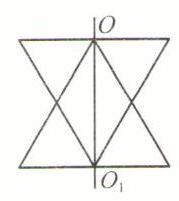
\includegraphics[width=0.2\textwidth]{bodyxb/src/bo_d20aucref24c73anc48g_198_1310_1512_179_201_0.jpg}
\end{center}


[第 118(5)题]

(5)如图,两个边长为 $a$ 的等边三角形有公共的高 $O{O}_{1}$ ,以直线 $O{O}_{1}$ 为轴将两个等边三角形旋转一周, 则所得旋转体的表面积为\blkda{}；

(6)已知圆锥的侧面积为 $S$ ,平行于底面的两个截面将圆锥的高分成相等的三段,则中间圆台的侧面积等于\blkda{}.

119. (1) 已知圆锥有一个内接圆柱, 此圆柱的底面在圆锥的底面上, 圆柱的高等于圆锥底面的半径,且圆柱的全面积:圆锥的底面积 $= 3 : 2$ ,求圆锥顶角的正切值；

(2)已知圆锥顶角是 ${120}^{ \circ  }$ ,求圆锥过两条母线的最大面积的截面和圆锥的轴所成的角.

120. (1) 已知圆锥的高 ${PO}$ 为 $\sqrt{2}\mathrm{{cm}}$ ,过顶点 $P$ 的一个截面 ${PAB}$ 与底面成 ${45}^{ \circ  }$ 角,且截面 ${PAB}$ 的面积为 $4{\mathrm{{cm}}}^{2}$ (如图),求此圆锥的侧面积;

\begin{center}
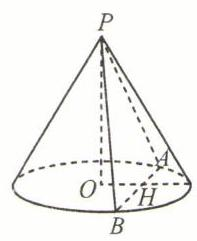
\includegraphics[width=0.2\textwidth]{bodyxb/src/bo_d20aucref24c73anc48g_199_1203_139_197_241_0.jpg}
\end{center}


[第 120(1)题]

(2)若过圆锥顶点的一个截面与圆锥的底面成 ${60}^{ \circ  }$ 角,截面截得圆锥底面的劣弧所对的圆心角为 ${120}^{ \circ  }$ ,底面圆心到截面的距离为 $3\mathrm{{dm}}$ ,求圆锥的侧面积及截面的面积.

\section*{(B)}

121. 将一个半圆围成一个圆锥的侧面,则两条母线间的最大夹角是(   )

(A) ${60}^{ \circ  }$ . (B) ${90}^{ \circ  }$ .

(C) ${120}^{ \circ  }$ . (D) ${150}^{ \circ  }$ .

122. 在轴截面为直角三角形的圆锥内作一内接圆柱,若圆柱的全面积等于圆锥的侧面积,则圆柱的高等于圆锥高的(   )

(A) $\dfrac{\sqrt{2}}{2}$ . (B) $\dfrac{2 - \sqrt{2}}{2}$ . (C) $\dfrac{1}{2}$ . (D) $\sqrt{2} - 1$ .

123. 已知圆锥母线长为 $p$ ,底面半径为 $R$ . 如果过圆锥顶点的截面的最大面积为 $\dfrac{1}{2}{p}^{2}$ ,那么比值 $R : p$ 应满足关系 (   )

(A) $\dfrac{R}{p} = \dfrac{\sqrt{2}}{2}$ . (B) $\dfrac{R}{p} \geq  \dfrac{\sqrt{2}}{2}$ . (C) $\dfrac{R}{p} > \dfrac{\sqrt{2}}{2}$ . (D) $\dfrac{R}{p} < \dfrac{\sqrt{2}}{2}$ .

124. 若过圆锥顶点的面积最大的截面是轴截面,且圆锥侧面展开图的圆心角为 $\alpha$ ,则 $\alpha$ 的取值范围是(   )

(A) $\left( {0,{2\pi }}\right)$ . (B) $\left( {0,\pi }\right)$ . (C) $\left( {0,\sqrt{2}\pi }\right\rbrack$ . (D) $\lbrack \sqrt{2}\pi ,{2\pi })$ .

125. 将圆心角为 ${120}^{ \circ  }$ 的扇形围成一个圆锥的侧面,则该圆锥轴截面顶角的余弦值为(   )

(A) 0 . (B) $\dfrac{1}{3}$ . (C) $\dfrac{5}{9}$ . (D) $\dfrac{7}{9}$ .

126. 已知平行于圆锥底面的平面把圆锥侧面分成面积相等的两部分,则所截得的小圆锥高与原圆锥高之比是(   )

(A) $1 : \sqrt{2}$ . (B) $1 : 2$ . (C) $1 : 2\sqrt{2}$ . (D) $1 : 4$ .

127. 若轴截面为直角三角形的圆锥的内接圆柱的全面积等于圆锥的侧面积, 则此圆锥的顶点到圆柱上底面的距离是此圆锥母线长的(   )

(A) $\dfrac{1}{4}$ . (B) $\dfrac{1}{3}$ . (C) $\dfrac{1}{2}$ . (D) $\dfrac{2}{3}$ .

128. 底面直径与高都是 1 的圆锥的内接正方体的棱长为(   )

(A) $\sqrt{2} + 1$ . (B) $\dfrac{\sqrt{2} + 1}{2}$ . (C) $\sqrt{2} - 1$ . (D) $\dfrac{1}{2}$ .

129. 面积为 $Q$ 的菱形,绕其一边旋转,则所得旋转体的表面积是 (   )

(A) ${\pi Q}$ . (B) ${2\pi Q}$ . (C) ${3\pi Q}$ . (D) ${4\pi Q}$ .

130. 已知两个母线长相等的圆锥的侧面展开图恰能拼成一个圆,且它们的侧面积之比为 $1 : 2$ ,则它们的高之比为 (   )

(A) $2 : 1$ . (B) $3 : 2$ . (C) $2\sqrt{2} : \sqrt{5}$ . (D) $5 : 2\sqrt{2}$ .

131. 由三条直线 $x = 1,x + y - 2 = 0$ 和 $x - y - 2 = 0$ 围成一个封闭的平面图形,求此平面图形绕 $y$ 轴旋转一周所得旋转体的表面积.

132. 已知圆锥底面直径 ${AB} = 2$ ,顶角 $\angle {APB} = {90}^{ \circ  }$ ,又底面半径 ${OC}\bot {AB}$ (如图),求:

(1)异面直线 ${AC}$ 与 ${PB}$ 所成的角；

(2)二面角 $B - {PA} - C$ 的正切值.

\begin{center}
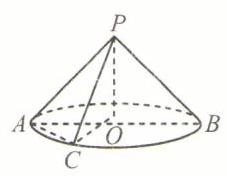
\includegraphics[width=0.2\textwidth]{bodyxb/src/bo_d20aucref24c73anc48g_200_489_657_227_176_0.jpg}
\end{center}


(第 132 题)

\begin{center}
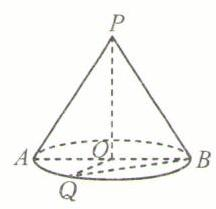
\includegraphics[width=0.2\textwidth]{bodyxb/src/bo_d20aucref24c73anc48g_200_975_623_216_209_0.jpg}
\end{center}


(第 133 题)

133. 已知圆锥的轴截面是一个等腰直角三角形 ${PAB},Q$ 是底面圆周上一点,且二面角 $A - {PB}$  $- Q$ 的正切值为 $\dfrac{\sqrt{6}}{3}$ (如图),求 $\angle {AOQ}$ 的大小 $(O$ 是底面圆心).

134. 已知圆锥底面的周长为 $C$ ,母线与底面所成的角为 ${60}^{ \circ  }$ ,将圆锥放倒在平面上,绕其顶点滚动一周,求圆锥的高旋转后所得的旋转面的面积.

135. 在边长为 $a$ 的正方形中,剪下一个扇形和一个圆,分别作为圆锥的侧面和底面,其中圆和扇形及正方形的两边相切 (如图),求圆锥的高.

\begin{center}
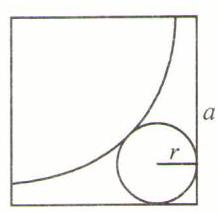
\includegraphics[width=0.2\textwidth]{bodyxb/src/bo_d20aucref24c73anc48g_200_1273_1196_219_213_0.jpg}
\end{center}


(第 135 题)

136. (1) 求底面半径为 $R$ ,高为 $h\left( {R < \sqrt{2}h}\right)$ 的圆锥的内接正四棱柱的表面积的最大值;

(2)圆锥底面半径为 $5\mathrm{{cm}}$ ,高为 ${12}\mathrm{{cm}}$ ,当它的内接圆柱的底面半径为何值时, 圆柱的全面积有最大值? 最大值是多少?

137. (1) 在顶点为 $P$ 的圆锥中,已知 ${OA},{OB}$ 是圆锥底面互相垂直的两条半径, $C$ 是母线 ${PB}$ 的中点,且 ${PB} = 3,{OA} = {OB} = 2$ ,求 $A$ , $C$ 两点在圆锥侧面上的最短距离；

(2)已知圆锥的底面半径 ${OA} = {10}\mathrm{{cm}}$ ,母线 ${PA} = {30}\mathrm{{cm}}$ ,由底面圆周上一点 $A$ 出发绕其侧面一周的最短路线的长度是多少? 最短路线上的点到底面的距离最大是多少?

\section*{(三)球}

\section*{【典型题型和解题技巧】}

“切”与“接”.

对于多面体、旋转体之间的“切”与“接”的问题,必须明确“切”或“接”的位置,明确有关元素间的数量关系,同时借助“剖面”图进行研究.

( 1 )正方体和它的内切球、外接球.

①正方体和它的内切球(如图 24).

\begin{center}
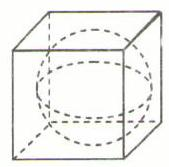
\includegraphics[width=0.2\textwidth]{bodyxb/src/bo_d20aucref24c73anc48g_201_314_262_169_167_0.jpg}
\end{center}


(图 24)

\begin{center}
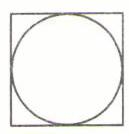
\includegraphics[width=0.2\textwidth]{bodyxb/src/bo_d20aucref24c73anc48g_201_680_294_129_134_0.jpg}
\end{center}


(图 25)

\begin{center}
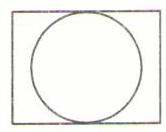
\includegraphics[width=0.2\textwidth]{bodyxb/src/bo_d20aucref24c73anc48g_201_1006_294_166_132_0.jpg}
\end{center}


(图 26)

常用的剖面有两种,一种是过球心且与正方体侧面平行的剖面,如图 25 ,它是一个正方形和它的内切圆,由图易知正方体棱长 $a$ 和内切球半径 $r$ 之间满足关系式 $a = {2r}$ ; 另一种是正方体的对角面和球的大圆, 如图 26.

②正方体和它的外接球 (如图 27).

\begin{center}
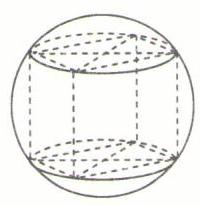
\includegraphics[width=0.2\textwidth]{bodyxb/src/bo_d20aucref24c73anc48g_201_410_735_201_205_0.jpg}
\end{center}


(图 27)

\begin{center}
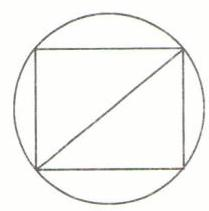
\includegraphics[width=0.2\textwidth]{bodyxb/src/bo_d20aucref24c73anc48g_201_871_725_209_211_0.jpg}
\end{center}


(图 28)

常用的剖面是正方体的对角面和球的大圆(如图 28). 由图易知,正方体棱长 $a$ 与外接球半径 $R$ 之间满足关系式 $\sqrt{3}a = {2R}$ .

(2)圆锥和它的内切球(如图 29).

\begin{center}
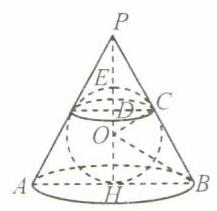
\includegraphics[width=0.2\textwidth]{bodyxb/src/bo_d20aucref24c73anc48g_201_438_1190_217_211_0.jpg}
\end{center}


(图 29)

\begin{center}
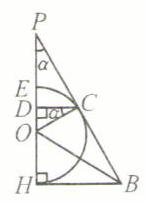
\includegraphics[width=0.2\textwidth]{bodyxb/src/bo_d20aucref24c73anc48g_201_913_1198_145_202_0.jpg}
\end{center}


(图 30)

常用的剖面是圆锥的轴截面(等腰三角形)和它的内切圆(球的大圆),或轴截面的一半(如图 30),可利用 ${OH} = {OC} = {OE},{BH} = {BC},\mathrm{{Rt}} \bigtriangleup  {PCO} \oslash  \mathrm{{Rt}} \bigtriangleup  {PHB},{CD}//{BH},{BO}$ 平分 $\angle {PBH}$ 等性质来解题.

例 1 圆锥的底面半径为 $R$ ,轴截面顶角为 ${2\alpha }$ ,球 $O$ 是它的内切球,如图 29,求内切球半径 $r$ .

解 设内切球半径为 $r$ ,在 $\mathrm{{Rt}}\bigtriangleup {BOH}$ 中,

$r = {OH} = R\tan \angle {OBH} = R\tan \dfrac{{90}^{ \circ  } - \alpha }{2} = R\tan \left( {{45}^{ \circ  } - \dfrac{\alpha }{2}}\right) .$

圆台和它的内切球 (如图 31).

\begin{center}
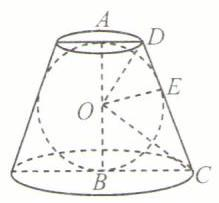
\includegraphics[width=0.2\textwidth]{bodyxb/src/bo_d20aucref24c73anc48g_201_416_1897_219_203_0.jpg}
\end{center}


(图 31)

\begin{center}
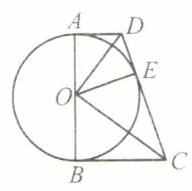
\includegraphics[width=0.2\textwidth]{bodyxb/src/bo_d20aucref24c73anc48g_201_895_1907_192_191_0.jpg}
\end{center}


(图 32)

常用的剖面是圆台的轴截面(等腰梯形)或轴截面的一半和它的内切圆(球的大圆),如图 32,可利用的性质有: ${AD} = {DE},{BC} = {CE},{OD},{OC}$ 分别平分 $\angle {ADE}$ 和 $\angle {BCE}$ 等,如果圆台的上、下底面半径分别为 ${r}_{1},{r}_{2}$ ,母线长为 $l$ ,内切球半径为 $R$ ,则 ${r}_{1} + {r}_{2} = l$ ,且由 ${DO} \bot  {CO}$ , ${OE} \bot  {CD}$ ,有 ${R}^{2} = {r}_{1} \cdot  {r}_{2}$ .

例 2 圆台的内切球半径为 $R$ ,且圆台的全面积和球面积之比为 $\dfrac{21}{8}$ ,求圆台的上、下底面半径 ${r}_{1},{r}_{2}$ .

解 设圆台母线为 $l$ ,则 $l = {r}_{1} + {r}_{2}$ .

$\therefore {S}_{\text{ 圆台全 }} = \pi \left( {{r}_{1} + {r}_{2}}\right)  \cdot  l + \pi {r}_{1}^{2} + \pi {r}_{2}^{2} = \pi \left\lbrack  {{\left( {r}_{1} + {r}_{2}\right) }^{2} + \left( {{r}_{1}^{2} + {r}_{2}^{2}}\right) }\right\rbrack$ ,

${S}_{\text{ 球 }} = {4\pi }{R}^{2} = {4\pi }{r}_{1}{r}_{2}.$

由题意,得 $\dfrac{2\left( {{r}_{1}^{2} + {r}_{2}^{2} + {r}_{1}{r}_{2}}\right) }{4{r}_{1}{r}_{2}} = \dfrac{21}{8}$ ,化简,得 $4{r}_{1}^{2} - {17}{r}_{1}{r}_{2} + 4{r}_{2}^{2} = 0$ ,

即 $\left( {4{r}_{1} - {r}_{2}}\right) \left( {{r}_{1} - 4{r}_{2}}\right)  = 0,\therefore {r}_{2} = 4{r}_{1}$ .

\begin{center}
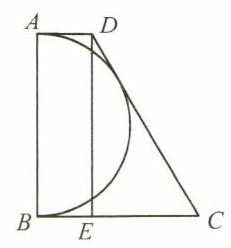
\includegraphics[width=0.2\textwidth]{bodyxb/src/bo_d20aucref24c73anc48g_202_1242_820_231_248_0.jpg}
\end{center}


(图 33)

代入 ${R}^{2} = {r}_{1}{r}_{2}$ ,得 $4{r}_{1}^{2} = {R}^{2}.\therefore {r}_{1} = \dfrac{R}{2},{r}_{2} = {2R}$ .

注意 ${R}^{2} = {r}_{1}{r}_{2}$ 也可由直角梯形转化为直角三角形而得,如图 33,

由 $D{E}^{2} = D{C}^{2} - E{C}^{2}$ ,得 $4{R}^{2} = {\left( {r}_{2} + {r}_{1}\right) }^{2} - {\left( {r}_{2} - {r}_{1}\right) }^{2} = 4{r}_{1}{r}_{2}$ ,

$\therefore {R}^{2} = {r}_{1}{r}_{2}$ .

(4)正棱锥和它的内切球.

球与正棱锥相切的切点, 分别在底面的中心和侧面的斜高上 (如图 34).

\begin{center}
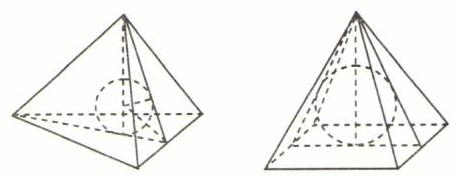
\includegraphics[width=0.3\textwidth]{bodyxb/src/bo_d20aucref24c73anc48g_202_302_1266_456_180_0.jpg}
\end{center}


(图 34)

\begin{center}
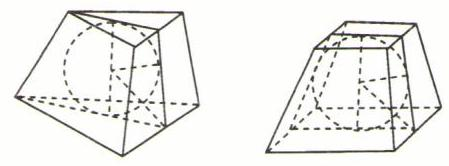
\includegraphics[width=0.3\textwidth]{bodyxb/src/bo_d20aucref24c73anc48g_202_884_1277_449_166_0.jpg}
\end{center}


(图 35)

(5)正棱台和它的内切球.

球与正棱台相切的切点, 分别在两底面中心和侧面的斜高上 (如图 35).

\section*{【训练题】}

\section*{(A)}

138. 已知球的两个平行截面的面积分别为 ${5\pi }$ 和 ${8\pi }$ ,它们位于球心的同一侧,且相距为 1 ,那么这个球的半径是(   )

(A) 4. (B) 3. (C) 2. (D) 5.

139. 湖面上漂着一个球,湖结冰后将球取出,冰面上留下了一个直径为 ${24}\mathrm{{cm}}$ ,深为 $8\mathrm{{cm}}$ 的空穴,则该球的半径是(   )

(A) $8\mathrm{{cm}}$ . (B) ${12}\mathrm{{cm}}$ . (C) ${13}\mathrm{{cm}}$ . (D) $8\sqrt{2}\mathrm{{cm}}$ .

140. 设地球半径为 $R$ ,在北纬 ${30}^{ \circ  }$ 圈上有甲、乙两地,它们的经度相差 ${120}^{ \circ  }$ ,则连接这两地的纬度线长为 (   )

(A) ${\pi R}$ . (B) ${2\pi R}$ . (C) $\dfrac{\sqrt{3}}{3}{\pi R}$ . (D) $\sqrt{3}{\pi R}$ .

141. 过球面上任意两点, 作球的大圆个数是 (   )

(A) 有且只有一个. (B) 有且只有两个.

(C) 无数个. (D) 一个或无穷多个.

142. (1)球的外切圆柱的全面积与球面面积之比为\blkda{}；

(2)已知等边圆柱、等边圆锥有相同的内切球,则内切球面积:圆柱全面积:圆锥全面积 $=$ \blkda{};

(3)一个球的半径为 $a$ ,放在墙角与两个墙面及地面都相切,那么球心与墙角顶点的距离是\blkda{}.

143. (1) 在母线长为 $a$ 的等边圆锥内有一个内切球,在这个球内又有一个内接正方体,则这个正方体的棱长是\blkda{}；

(2)已知长方体共顶点的三个面的面积分别为 $\sqrt{3},\sqrt{5},\sqrt{15}$ ,则它的外接球的面积为\blkda{}；

(3)球面上有四个点 $P,A,B,C$ ,如果 ${PA},{PB},{PC}$ 两两互相垂直,且 ${PA} = {PB} = {PC} =$  $a$ ,那么这个球面的面积是\blkda{}.

\section*{(B)}

144. 已知过球面上 $A,B,C$ 三点的截面和球心的距离等于球半径的一半,且 ${AB} = {BC} = {CA} =$ 2, 则球面面积是 (   )

(A) $\dfrac{16}{9}\pi$ . (B) $\dfrac{8}{3}\pi$ . (C) ${4\pi }$ . (D) $\dfrac{64}{9}\pi$ .

145. 自半径为 $R$ 的球面上一点 $Q$ 作球的互相垂直的三条弦 ${QA},{QB},{QC}$ ,则 $Q{A}^{2} + Q{B}^{2} +$  $Q{C}^{2}$ 等于(   )

(A) $8{R}^{2}$ . (B) $4{R}^{2}$ . (C) $2{R}^{2}$ . (D) ${R}^{2}$ .

146. 若一个球的外切圆锥的高是这个球直径的 2 倍, 那么其外切圆锥的全面积与球面面积之比是(   )

(A) $2 : 1$ . (B) $2 : 3$ . (C) $4 : 1$ . (D) $4 : 9$ .

147. 四个半径为 $R$ 的球两两外切,其中三个放在水平桌面上,第四个放在这三个之上,则第四个球的最高点离开桌面的高度是(   )

(A) ${4R}$ . (B) $\left( {1 + \dfrac{\sqrt{6}}{3}}\right) R$ . (C) $2\left( {1 + \dfrac{\sqrt{2}}{3}}\right) R$ . (D) $2\left( {1 + \dfrac{\sqrt{6}}{3}}\right) R$ .

148. (1) 半径为 $5\mathrm{{cm}}$ 的球内有一个内接圆锥,这个圆锥的高为 $7\mathrm{{cm}}$ ,则这个圆锥的侧面积为\blkda{}；

(2)球的外切圆台的两底半径分别为 $R,r$ ,则球的表面积为\blkda{}.

149. 在半径为 ${30}\mathrm{{cm}}$ 的球面上有三个点 $A,B,C$ ,它们之间的距离依次是 ${20}\mathrm{{cm}},{12}\mathrm{{cm}},{16}\mathrm{{cm}}$ , 求过 $A,B,C$ 三点的平面与球心间的距离.

150. (1) 已知各棱长都相等的三棱锥内接在一个表面积为 ${36\pi }$ 的球内,求这个棱锥的高;

(2)已知半球内有一内接正方体,试求这个半球面面积与正方体表面积之比；

(3)已知圆锥的全面积是其内切球表面积的 2 倍,求圆锥的侧面积和底面积的比.

151. 已知正四棱锥 $P - {ABCD}$ 内接于球 $O$ ,它的底面边长为 $a$ ,侧棱和底面成 $\alpha$ 角 (如图),求球的面积.

\begin{center}
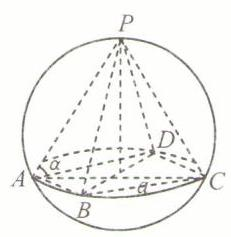
\includegraphics[width=0.2\textwidth]{bodyxb/src/bo_d20aucref24c73anc48g_204_509_607_231_237_0.jpg}
\end{center}


(第 151 题)

\begin{center}
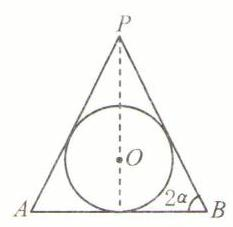
\includegraphics[width=0.2\textwidth]{bodyxb/src/bo_d20aucref24c73anc48g_204_902_620_233_227_0.jpg}
\end{center}


(第 152 题)

152. 已知半径为 $R$ 的球的外切圆锥的轴截面底角为 ${2\alpha }$ (如图).

(1)求证:圆锥的全面积为 $\dfrac{{2\pi }{R}^{2}}{{\tan }^{2}\alpha \left( {1 - {\tan }^{2}\alpha }\right) }$ ；

(2)当 $\tan \alpha$ 为何值时,外切圆锥全面积有最小值,最小值是多少？

*153. 已知圆台有一个内切球.

(1)求证:圆台的高是圆台的上、下底面直径的比例中项；

(2)若圆台母线与下底面成 $\alpha$ 角,求圆台侧面积与内切球面积之比；

(3)若圆台侧面积与内切球面积之比为 $4 : 3$ ,求圆台母线与底面所成的角；

(4)若内切球半径为 $R$ ,且圆台的全面积和内切球面积之比为 $p : 1$ , 求圆台的上、下底面半径.

\begin{center}
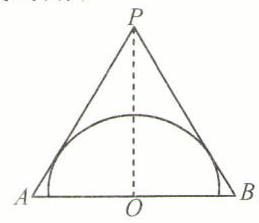
\includegraphics[width=0.2\textwidth]{bodyxb/src/bo_d20aucref24c73anc48g_204_1214_1348_259_223_0.jpg}
\end{center}


(第 154 题)

154. 一个球的大圆在圆锥的底面上, 且球与圆锥侧面相切 (如图), 若圆锥底面半径为 $R$ ,且 ${S}_{\text{ 圆锥全 }} = {S}_{\text{ 球 }}$ ,求圆锥的表面积.

\section*{三、多面体和旋转体的体积}

\section*{(一) 棱柱和圆柱的体积}

\section*{【典型题型和解题技巧】}

1. 平行六面体的“选底”.

由于棱柱的体积等于底面积与高的乘积, 而平行六面体的各个面均可作为底面, 因此, 平行六面体的“选底”就显得十分重要.

例 1 已知斜三棱柱 ${ABC} - {A}_{1}{B}_{1}{C}_{1}$ 的侧面 $B{B}_{1}{C}_{1}C$ 的面积为 $S$ ,侧棱 $A{A}_{1}$ 到侧面 $B{B}_{1}{C}_{1}C$ 的距离为 $a$ (如图 36),求该三棱柱的体积.

\begin{center}
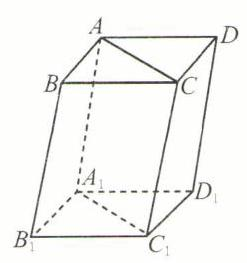
\includegraphics[width=0.2\textwidth]{bodyxb/src/bo_d20aucref24c73anc48g_205_1169_199_247_263_0.jpg}
\end{center}


(图 36)

解 在斜三棱柱 ${ABC} - {A}_{1}{B}_{1}{C}_{1}$ 的一侧补上一个三棱柱 ${ACD}$ - ${A}_{1}{C}_{1}{D}_{1}$ ,使之成为一个平行六面体 $A{A}_{1}{D}_{1}D - B{B}_{1}{C}_{1}C$ ,显然,它的体积为 ${aS}$ ,于是斜三棱柱 ${ABC} - {A}_{1}{B}_{1}{C}_{1}$ 的体积为 $\dfrac{1}{2}{aS}$ .

注意 在本例的解法中运用了“补形”的技巧. “补形”在求几何体的体积中常被应用.

2. 棱柱中的“定高”.

“高”在棱柱体积的计算中至关重要,而求高的关键在于确定“垂足”的位置.

\begin{center}
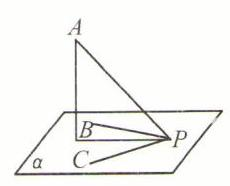
\includegraphics[width=0.2\textwidth]{bodyxb/src/bo_d20aucref24c73anc48g_205_1186_693_230_186_0.jpg}
\end{center}


(图 37)

本单元较多用到如下事实: 若平面 $\alpha$ 的斜线 ${AP}$ 和 $\alpha$ 内的两条射线 ${PB}$ , ${PC}$ 交成相等的锐角,则 ${PA}$ 在 $\alpha$ 内的射影是 $\angle {BPC}$ 的平分线 (如图 37).

例 2 已知平行六面体 ${ABCD} - {A}_{1}{B}_{1}{C}_{1}{D}_{1}$ 的底面是边长为 $a$ 的正方形,侧棱 $A{A}_{1}$ 长为 $b$ ,且 $\angle A{A}_{1}{B}_{1} = \angle A{A}_{1}{D}_{1} = {60}^{ \circ  }$ ,如图 38,求平行六面体的体积.

解 作 ${AO} \bot$ 底面 ${A}_{1}{B}_{1}{C}_{1}{D}_{1},O$ 为垂足,则由已知条件得 ${A}_{1}O$ 平分 $\angle {B}_{1}{A}_{1}{D}_{1}$ ,作 ${OE}\bot {A}_{1}{B}_{1}$ 于点 $E$ ,连接 ${AE}$ ,则 ${AE}\bot {A}_{1}{B}_{1}$ .

\begin{center}
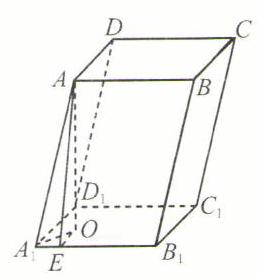
\includegraphics[width=0.2\textwidth]{bodyxb/src/bo_d20aucref24c73anc48g_205_1158_1030_258_278_0.jpg}
\end{center}


(图 38)

$\because A{A}_{1} = b,\angle A{A}_{1}{B}_{1} = {60}^{ \circ  },\therefore {A}_{1}E = \dfrac{b}{2},{AE} = \dfrac{\sqrt{3}}{2}b.$

而 ${OE} = \dfrac{b}{2},\therefore {AO} = \dfrac{\sqrt{2}}{2}b$ ,于是平行六面体的体积为 $\dfrac{\sqrt{2}}{2}{a}^{2}b$ .

\section*{【训练题】}

\section*{(A)}

155. 已知正四棱柱的底面积为 $P$ ,过两相对侧棱的截面面积为 $Q$ ,则正四棱柱的体积为(   )

(A) $\dfrac{\sqrt{2P}}{2}Q$ . (B) $\dfrac{\sqrt{2Q}}{2}P$ . (C) $\sqrt{P}Q$ . (D) $\sqrt{Q}P$ .

156. 正方体 ${EFGH} - {E}_{1}{F}_{1}{G}_{1}{H}_{1}$ 的棱长为 $2,M$ 为棱 ${E}_{1}{F}_{1}$ 的中点,过 $E,M,H$ 三点的截面将此正方体分割成的大小两部分的体积比是(   )

(A) $5 : 1$ . (B) $4 : 1$ . (C) $3 : 1$ . (D) $2 : 1$ .

157. 已知圆柱的底面积为 $S$ ,轴截面面积为 $T$ ,则圆柱的体积为(   )

(A) $\dfrac{T}{2}\sqrt{\pi S}$ . (B) $\dfrac{S}{2}\sqrt{\pi T}$ . (C) $\sqrt{\pi TS}$ . (D) $\pi \sqrt{TS}$ .

158. 若一等边圆柱的轴截面面积为 $Q$ ,则该圆柱的体积为 (   )

(A) ${\pi Q}\sqrt{Q}$ . (B) $\dfrac{\pi }{2}Q\sqrt{Q}$ . (C) $\dfrac{\pi }{3}Q\sqrt{Q}$ . (D) $\dfrac{\pi }{4}Q\sqrt{Q}$ .

159. 先作一个圆柱的内接正三棱柱,再作这个三棱柱的内切圆柱,则这两个圆柱的体积之比是(   )

(A) $\pi  : 1$ . (B) $4 : 1$ . (C) $2 : 1$ . (D) $\sqrt{2} : 1$ .

160. 已知圆柱的侧面展开图是边长为 4 和 6 的矩形, 则该圆柱的体积为 (   )

(A) $\dfrac{24}{\pi }$ . (B) $\dfrac{36}{\pi }$ . (C) $\dfrac{24}{\pi }$ 或 $\dfrac{60}{\pi }$ . (D) $\dfrac{24}{\pi }$ 或 $\dfrac{36}{\pi }$ .

161. 已知一个正六棱柱的底面边长是 $2\sqrt{3}$ ,最长的对角线为 8,则这个正六棱柱的体积是(   )

(A) $2\sqrt{3}$ . (B) ${48}\sqrt{3}$ . (C) ${72}\sqrt{3}$ . (D) ${96}\sqrt{3}$ .

162. (1) 已知长方体交于一个顶点的三个面的面积分别为 $\sqrt{2},\sqrt{3},\sqrt{6}$ ,则这个长方体的体积等于\blkda{}；

(2)将正方体的棱长增加 $2\mathrm{{cm}}$ ,体积便增加 ${98}{\mathrm{{cm}}}^{3}$ ,那么原来正方体的体积为\blkda{} ${\mathrm{{cm}}}^{3}$ ；

(3)长方体共顶点的三个面的面积分别是 ${S}_{1},{S}_{2},{S}_{3}$ ,它的体积为\blkda{}.

163. (1)若圆柱的轴截面是面积为 $2{a}^{2}$ 的正方形,该圆柱的体积是\blkda{}；

(2)若等边圆柱的轴截面的面积为 ${36}{\mathrm{{cm}}}^{2}$ ,则它的内接正六棱柱的体积为\blkda{}；

(3)已知圆柱的底面半径为 $r$ ,高为 $h$ ,则以圆柱轴截面为一个侧面的内接三棱柱的最大体积等于\blkda{}；

(4)已知圆柱的侧面积为 $\pi {a}^{2}$ ,体积为 $\pi {b}^{2}$ ,则其底面半径为\blkda{}；

(5)高分别是 $a$ 和 $b$ 的两个圆柱的侧面展开图是全等图形,如果前一个圆柱的体积是后一个圆柱体积的一半,那么 $a : b$ \blkda{}；

(6)一个圆柱的高是 $H$ ,它的侧面展开图中母线与对角线的夹角是 ${60}^{ \circ  }$ ,则它的体积是\blkda{}.

164. (1) 已知三棱柱底面的三边 ${AB},{BC},{CA}$ 分别为 $5\mathrm{{cm}},3\mathrm{{cm}},4\mathrm{{cm}}$ ,侧棱 $A{A}^{\prime }$ 长为 ${10}\mathrm{{cm}}$ , 且侧棱与底面成 ${45}^{ \circ  }$ 角,求该三棱柱的体积；

( 2 )在斜三棱柱 ${ABC} - {A}_{1}{B}_{1}{C}_{1}$ 中,已知侧面 $A{A}_{1}{B}_{1}B$ 与侧面 $A{A}_{1}{C}_{1}C$ 成 ${60}^{ \circ  }$ 角,且它们的面积之比为 $8 : 5$ ,又这个棱柱的侧面积为 ${60}{\mathrm{{cm}}}^{2}$ ,体积为 ${15}\sqrt{3}{\mathrm{{cm}}}^{3}$ ,求它的侧棱长.

\section*{(B)}

165. 若正四棱锥的底面积是 $S$ ,侧面积是 $Q$ ,则它的体积是 (   )

(A) $\dfrac{S}{3}\sqrt{Q - S}$ . (B) $\dfrac{1}{3}\sqrt{S\left( {{Q}^{2} - {S}^{2}}\right) }$ . (C) $\dfrac{1}{6}\sqrt{S\left( {{Q}^{2} - {S}^{2}}\right) }$ . (D) $\dfrac{1}{6}\sqrt{S\left( {{16}{Q}^{2} - {S}^{2}}\right) }$ .

166. 若正四棱柱的对角线和侧面所成角为 ${30}^{ \circ  }$ ,底面边长为 $a$ ,则它的体积是(   )

(A) $\dfrac{\sqrt{2}}{3}{a}^{3}$ . (B) $\sqrt{2}{a}^{3}$ . (C) $\dfrac{\sqrt{3}}{3}{a}^{3}$ . (D) $\sqrt{3}{a}^{3}$ .

167. 已知一个平行六面体相交于一个顶点的三条棱长为 $a,b,c$ ,三条棱中两两所夹的角都为 ${60}^{ \circ  }$ ,则此平行六面体的体积为(   )

(A) $\dfrac{\sqrt{2}}{2}{abc}$ . (B) $\dfrac{\sqrt{3}}{2}{abc}$ . (C) abc. (D) $\dfrac{\sqrt{6}}{2}{abc}$ .

168. (1)已知圆柱轴截面的对角线长 1,为了使圆柱的侧面积最大,轴截面对角线与底面所成角为\blkda{},此时圆柱的体积为\blkda{}；

( 2 )在斜三棱柱 ${ABC} - {A}_{1}{B}_{1}{C}_{1}$ 中,已知底面 $\bigtriangleup  {ABC}$ 的 $\angle {ACB}$ 为 ${90}^{ \circ  },{AC}$ 长为 1,侧面 ${A}_{1}{AC}{C}_{1}$ 是矩形,侧面 ${B}_{1}{BC}{C}_{1}$ 的面积为 $2\sqrt{3}$ ,则此三棱柱的体积 $V$ 等于\blkda{}.

169. (1) 在正三棱柱 ${ABC} - {A}_{1}{B}_{1}{C}_{1}$ 中,已知侧棱长为 $3,P$ 为侧棱 $A{A}_{1}$ 上一点,且 ${AP} = 1$ , $P{C}_{1}$ 与面 $A{A}_{1}{B}_{1}B$ 成 ${30}^{ \circ  }$ 角 (如图),求这个正三棱柱的体积;

\begin{center}
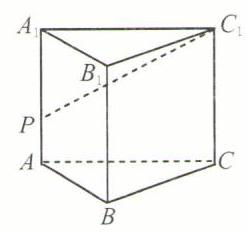
\includegraphics[width=0.2\textwidth]{bodyxb/src/bo_d20aucref24c73anc48g_207_444_895_247_232_0.jpg}
\end{center}


[第 169(1)题]

\begin{center}
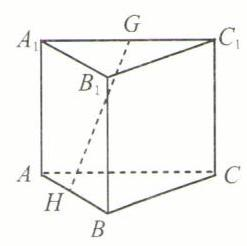
\includegraphics[width=0.2\textwidth]{bodyxb/src/bo_d20aucref24c73anc48g_207_950_879_247_246_0.jpg}
\end{center}


[第 169(2)题]

(2)在正三棱柱 ${ABC} - {A}_{1}{B}_{1}{C}_{1}$ 中,已知 $H,G$ 分别为 ${AB},{A}_{1}{C}_{1}$ 的中点,且 ${HG} = 2\mathrm{{cm}}$ , ${HG}$ 与 ${BC}$ 所成的角为 ${60}^{ \circ  }$ (如图),求三棱柱的体积.

170. (1) 已知三棱柱 ${ABC} - {A}_{1}{B}_{1}{C}_{1}$ 的底面是边长为 $a$ 的正三角形,侧棱长为 $b,\angle {A}_{1}{AB} = \angle {A}_{1}{AC} = {45}^{ \circ  }$ ,求三棱柱的侧面积和体积；

\begin{center}
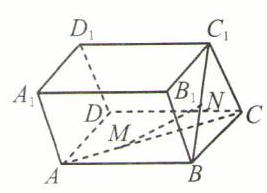
\includegraphics[width=0.2\textwidth]{bodyxb/src/bo_d20aucref24c73anc48g_207_1170_1322_267_193_0.jpg}
\end{center}


[第 170(2)题]

(2)已知一个平行六面体 ${ABCD} - {A}_{1}{B}_{1}{C}_{1}{D}_{1}$ 的底面 ${ABCD}$ 和侧面 ${BC}{C}_{1}{B}_{1}$ 都是正方形,且二面角 ${B}_{1} - {BC} - A$ 为 ${60}^{ \circ  },M,N$ 分别在面对角线 ${AC},B{C}_{1}$ 上,且 ${AM} = {BN}$ (如图).

①求证: ${MN}//$ 侧面 ${DC}{C}_{1}{D}_{1}$ ,

②若 ${BN} : {N{C}_{1}} = 1 : 3,{MN} = \dfrac{\sqrt{14}}{4}$ ,求此平行六面体的体积.

171. (1) 斜三棱柱一个侧面的面积为 $S$ ,并且该侧面到它相对棱间的距离为 $a$ ,求斜三棱柱的体积;

\begin{center}
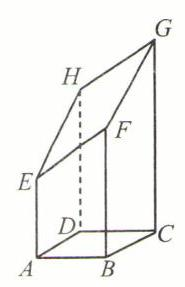
\includegraphics[width=0.2\textwidth]{bodyxb/src/bo_d20aucref24c73anc48g_207_1234_1768_185_287_0.jpg}
\end{center}


[第 171(2)题]

(2)已知 ${EFGH}$ 是长方体 ${ABCD} - {A}_{1}{B}_{1}{C}_{1}{D}_{1}$ 的一个截面,且 ${AB}$  $= 4,{BC} = 3,{AE} = 5,{BF} = 8,{CG} = {12}$ (如图).

①求证: ${EFGH}$ 是菱形,

②求多面体 ${ABCD} - {EFGH}$ 的体积.

172. 在 $▱{ABCD}$ 中,已知 ${AD} = a,{AB} = {2a},\angle {DAB} =$  ${60}^{ \circ  },M,N$ 分别为 ${AB},{CD}$ 的中点,以 ${MN}$ 为轴将 $▱{AMND}$ 旋转 ${120}^{ \circ  }$ (如图),求三棱柱 ${CDN} - {BAM}$ 的体积.

\begin{center}
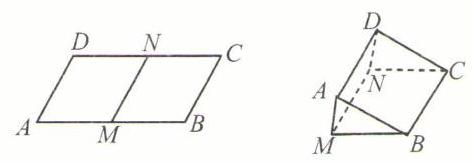
\includegraphics[width=0.4\textwidth]{bodyxb/src/bo_d20aucref24c73anc48g_208_1006_151_472_163_0.jpg}
\end{center}


(第 172 题)

173. 已知圆柱的高为 $2\mathrm{{cm}}$ ,体积为 ${98\pi }{\mathrm{{cm}}}^{3}$ ,一个正方形 ${ABCD}$ 的两个顶点 $A,D$ 在上底圆周上,另两个顶点 $B,C$ 在下底圆周上 (如图),求正方形 ${ABCD}$ 的面积.

\begin{center}
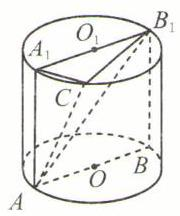
\includegraphics[width=0.2\textwidth]{bodyxb/src/bo_d20aucref24c73anc48g_208_967_550_180_216_0.jpg}
\end{center}


(第 174 题)

\begin{center}
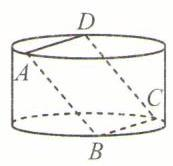
\includegraphics[width=0.2\textwidth]{bodyxb/src/bo_d20aucref24c73anc48g_208_496_601_173_166_0.jpg}
\end{center}


(第 173 题)

174. 已知 $A{A}_{1}{B}_{1}B$ 是圆柱的轴截面, $C$ 是上底面圆周上一点 (如图),

(1)若圆柱的体积为 $Q$ ,求棱锥 $A - {A}_{1}{B}_{1}C$ 的体积的最大值；

(2)若棱锥 $A - {A}_{1}{B}_{1}C$ 的体积；圆柱体积 $= 1 : 2\sqrt{3}\pi$ ,求二面角 ${B}_{1} - A{A}_{1} - C$ 的大小.

\section*{(二) 棱锥和圆锥的体积}

\section*{【典型题型和解题技巧】}

1. “比”.

棱锥、圆锥的横截面 (平行于底的截面) 有如下性质 (图 39):

\begin{center}
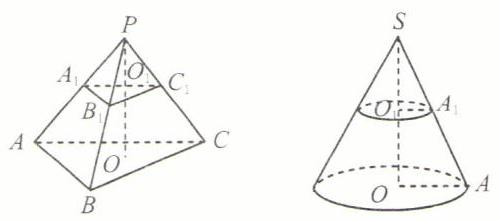
\includegraphics[width=0.4\textwidth]{bodyxb/src/bo_d20aucref24c73anc48g_208_579_1377_500_221_0.jpg}
\end{center}


(图 39)

(1) $\dfrac{{S}_{\text{ 小锥底 }}}{{S}_{\text{ 大锥底 }}} = \dfrac{{S}_{\text{ 小锥侧 }}}{{S}_{\text{ 大锥侧 }}} = \dfrac{{S}_{\text{ 小锥全 }}}{{S}_{\text{ 大锥全 }}} =$ 对应线段平方之比.

(2) $\dfrac{{V}_{\text{ 小锥 }}}{{V}_{\text{ 大锥 }}} =$ 对应线段立方之比.

例 1 平行于圆锥底面的截面将圆锥分为体积相等的两部分, 求这两部分的侧面积之比.

解 设截面、底面的半径分别为 $r,R$ ,

由题意得 $\dfrac{{V}_{\text{ 小锥 }}}{{V}_{\text{ 大锥 }}} = \dfrac{1}{2} = \dfrac{{r}^{3}}{{R}^{3}},\therefore \dfrac{r}{R} = \dfrac{1}{\sqrt[3]{2}}$ ,则 $\dfrac{{S}_{\text{ 小锥侧 }}}{{S}_{\text{ 大锥侧 }}} = \dfrac{1}{\sqrt[3]{4}}$ ,

$\therefore \dfrac{{S}_{\text{ 小锥侧 }}}{{S}_{\text{ 人牡侧 }} - {S}_{\text{ 小锥侧 }}} = \dfrac{1}{\sqrt[3]{4 - 1}}$ . 故这两部分的侧面积之比为 $1 : \left( {\sqrt[3]{4} - 1}\right)$ .

例 2 棱台的上底面面积为 ${16\pi }$ ,下底面面积为 ${64\pi }$ ,求棱台被它的中截面分成的上、下两部分的体积之比.

解 如图 40,将棱台回归到棱锥, $A{A}_{1},B{B}_{1},C{C}_{1}$ 分别是小锥、中锥、大锥底面上的对应线段, 则

\begin{center}
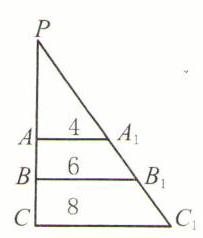
\includegraphics[width=0.2\textwidth]{bodyxb/src/bo_d20aucref24c73anc48g_209_1284_256_203_238_0.jpg}
\end{center}


(图 40)

${V}_{ + } : {V}_{ + } : {V}_{ + } = {4}^{3} : {6}^{3} : {8}^{3} = {2}^{3} : {3}^{3} : {4}^{3} = 8 : {27} : {64}$ ,

$\therefore \left( {{V}_{ \oplus  } - {V}_{ \land  }}\right)  : \left( {{V}_{ 大 } - {V}_{ \oplus  }}\right)  = \left( {{27} - 8}\right)  : \left( {{64} - {27}}\right)  = {19} : {37}$ ,

即上、下两部分体积之比为 ${19} : {37}$ .

注意 在遇到有关锥体、台体被横截面分成的面积、体积之比的问题时, 尽量避免直接运算, 宜运用有关的比例性质求解.

2. “割”与“补”.

当给出的几何体比较复杂, 有关的计算公式无法运用, 或几何体并不复杂, 但条件中的已知元素彼此离散时,我们可以采用“割”“补”的技巧,化复杂几何体为简单几何体(柱、锥、台), 或化离散为集中,给解题提供便利.

(1)几何体的“分割”.

例 3 如图 41,在三棱锥 $S - {ABC}$ 中, ${SA} = {18},{BC} = {16}$ ,其余棱长均为 17 ,求三棱锥的体积.

解 设 ${BC}$ 中点为 $M$ ,连接 ${SM},{AM}$ ,显然, ${BC} \bot  {AM},{BC} \bot  {SM}$ ,则 ${BC} \bot$ 平面 ${SAM}$ .

$\because {SB} = {SC} = {17},{BC} = {16},\therefore {BM} = 8$ ,则 ${SM} = {15}$ .

\begin{center}
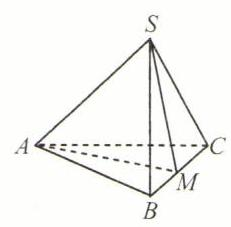
\includegraphics[width=0.2\textwidth]{bodyxb/src/bo_d20aucref24c73anc48g_209_1246_1109_231_227_0.jpg}
\end{center}


(图 41)

同理 ${AM} = {15},\bigtriangleup {SAM}$ 的边 ${SA}$ 上的高为

$\sqrt{A{M}^{2} - {\left( \dfrac{SA}{2}\right) }^{2}} = \sqrt{{15}^{2} - {9}^{2}} = {12},$

$\therefore {V}_{S - {ABC}} = {V}_{B - {SAM}} + {V}_{C - {SAM}}$

\[
= \dfrac{1}{3}{S}_{\bigtriangleup {SAM}} \cdot  \left( {{BM} + {CM}}\right)  = \dfrac{1}{3}{S}_{\bigtriangleup {SAM}} \cdot  {BC}
\]

\[
= \dfrac{1}{3} \cdot  \dfrac{1}{2} \cdot  {18} \cdot  {12} \cdot  {16} = {576}.
\]

注意 本例解中把一个三棱锥分割为两个三棱锥,它们有公共的底 $\bigtriangleup {SAM}$ ,而高的和恰为 ${BC}$ ,它的长度是已知的,因而计算简便. 如果用常规解法,计算难免繁冗.

例 4 求证: 四面体的两组对棱的四个中点共面, 且该平面把四面体分成等积的两部分.

分析 如图 42, $M,N,P,Q$ 分别为棱 ${AB},{AD},{BC},{CD}$ 的中点,这四点共面显而易见,但四面体被平面 ${MNQP}$ 分成的两部分体积计算较为困难. 考察几何体 ${AMPCQN}$ ,若过 ${MN}$ 作平面 ${NMR}$ 与平面 ${PQC}$ 平行,其中 $R$ 是该平面与棱 ${AC}$ 的交点,则可以验证 $R$ 是 ${AC}$ 的中点. 就把这个几何体分割成一个三棱柱和一个三棱锥, 它们的体积不难计算.

\begin{center}
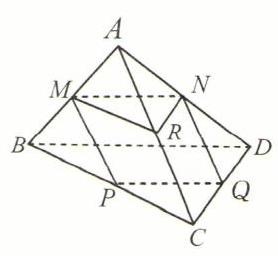
\includegraphics[width=0.2\textwidth]{bodyxb/src/bo_d20aucref24c73anc48g_209_1193_1751_278_256_0.jpg}
\end{center}


(图 42)

证明 由题设, $M,N$ 分别为 ${AB},{AD}$ 的中点,故 ${MN}//{BD}$ ,同理 ${PQ}//{BD}$ ,则 ${MN}//{PQ}$ ,点 $M,N,P,Q$ 共面. 设 $\bigtriangleup {BCD}$ 的面积为 $S$ ,点 $A$ 到底面 ${CBD}$ 的距离为 $h$ ,则

${V}_{A - {MNR}} = \dfrac{1}{3}{S}_{\bigtriangleup {MNR}} \cdot  \dfrac{1}{2}h = \dfrac{1}{3} \cdot  \dfrac{S}{4} \cdot  \dfrac{h}{2} = \dfrac{1}{24}{Sh},$

${V}_{{MNR} - {PQC}} = {S}_{\bigtriangleup {PQC}} \cdot  \dfrac{1}{2}h = \dfrac{S}{4} \cdot  \dfrac{h}{2} = \dfrac{1}{8}{Sh}.$

$\therefore {V}_{AMPCQN} = \left( {\dfrac{1}{24} + \dfrac{1}{8}}\right) {Sh} = \dfrac{1}{6}{Sh} = \dfrac{1}{2}{V}_{A - {BCD}}$ .

这就证明了平面 ${MNQP}$ 将四面体 ${ABCD}$ 分成了等积的两部分.

(2)几何体的“补形”.

例 5 四面体 $S - {ABC}$ 的三组对棱分别相等,且依次为 $2\sqrt{5},\sqrt{13},5$ ,求该四面体的体积.

解 由已知对棱相等, 将四面体 “补” 成如图 43 所示的长方体, 使四面体对棱分别为长方体相对面的对角线. (请同学们思考这样放置的合理性)

\begin{center}
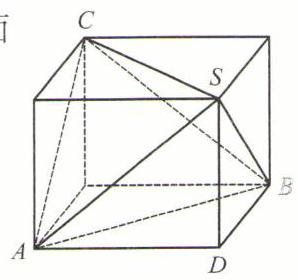
\includegraphics[width=0.2\textwidth]{bodyxb/src/bo_d20aucref24c73anc48g_210_1234_606_298_280_0.jpg}
\end{center}


(图 43)

设长方体三条棱长分别为 $x,y,z$ ,

则 $\left\{  \begin{array}{l} {x}^{2} + {y}^{2} = {\left( 2\sqrt{5}\right) }^{2}, \\  {y}^{2} + {z}^{2} = {\left( \sqrt{13}\right) }^{2}, \\  {z}^{2} + {x}^{2} = {5}^{2}, \end{array}\right.$ 解得 $\left\{  \begin{array}{l} x = 4, \\  y = 2, \\  z = 3. \end{array}\right.$

那么 ${V}_{\text{ 四面体 }} = {V}_{\text{ 长方体 }} - 4{V}_{D - \mathrm{{SAB}}} = {V}_{\text{ 长方体 }} - 4 \cdot  \dfrac{1}{6}{V}_{\text{ 长方体 }} = \dfrac{1}{3}{V}_{\text{ 长方体 }} = 8$ .

3. 体积法.

体积有时可以作为一种中介, 用来沟通有关元素之间的关系, 从而完成计算或证明. 其方法主要是借助于体积的相等,即所谓“等积”. 等积有两种:一种是“自等”,即借助于同一个几何体体积的不同算法；另一种是“互等”,即借助于两个体积相等的几何体.

(1) 体积的“自等”.

例 6 在棱长为 $a$ 的正方体 ${ABCD} - {A}_{1}{B}_{1}{C}_{1}{D}_{1}$ 中,求点 ${D}_{1}$ 到截面 ${C}_{1}{BD}$ 的距离.

解 如图 44,连接 ${D}_{1}B$ ,设点 ${D}_{1}$ 到截面 ${C}_{1}{BD}$ 的距离为 $h$ ,

\begin{center}
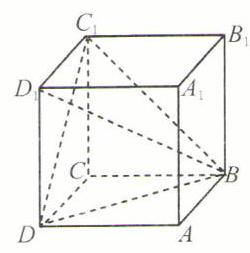
\includegraphics[width=0.2\textwidth]{bodyxb/src/bo_d20aucref24c73anc48g_210_1241_1414_250_253_0.jpg}
\end{center}


(图 44)

则 ${V}_{{D}_{1} - {C}_{1}{BD}} = \dfrac{1}{3}{S}_{\bigtriangleup {C}_{1}{BD}} \cdot  h = \dfrac{1}{3} \cdot   \cdot  \dfrac{\sqrt{3}}{4}{\left( \sqrt{2}a\right) }^{2}h = \dfrac{\sqrt{3}}{6}{a}^{2}h$ ,

${V}_{B - {C}_{1}{D}_{1}D} = \dfrac{1}{3}{S}_{\bigtriangleup {C}_{1}{D}_{1}D} \cdot  {BC} = \dfrac{1}{6}{a}^{3}.$

而 ${V}_{{D}_{1} - {C}_{1}{BD}} = {V}_{B - {C}_{1}{D}_{1}D},\therefore \dfrac{\sqrt{3}}{6}{a}^{2}h = \dfrac{1}{6}{a}^{3}$ ,得 $h = \dfrac{\sqrt{3}}{3}a$ .

$\therefore$ 点 ${D}_{1}$ 到截面 ${C}_{1}{BD}$ 的距离为 $\dfrac{\sqrt{3}}{3}a$ .

注意 体积“自等”的技巧主要用于三棱锥, 这是由于求体积时, 三棱锥的任何一个面都可以作为底面.

在求点到平面的距离或求两条异面直线的距离(转化为平行的直线和平面的距离)时,有时可用体积的“自等”法.

(2) 体积的“互等”.

例 7 设三棱柱 ${A}_{1}{B}_{1}{C}_{1} - {A}_{2}{B}_{2}{C}_{2}$ 被垂直于侧棱的平面 ${ABC}$ 所截,如图 45. 截面 $\bigtriangleup {ABC}$ 的面积为 $S,A{A}_{1} = {h}_{1},B{B}_{1} = {h}_{2},C{C}_{1} = {h}_{3}$ ,几何体 ${ABC} - {A}_{1}{B}_{1}{C}_{1}$ 的体积为 $V$ ,求证: $V = \dfrac{1}{3}S$  $\left( {{h}_{1} + {h}_{2} + {h}_{3}}\right)$ .

证明 利用分割及等积变形. 连接 $A{B}_{1},{B}_{1}C,{A}_{1}C$ ,把几何体 ${ABC} - {A}_{1}{B}_{1}{C}_{1}$ 分成三个四面体,则

\begin{center}
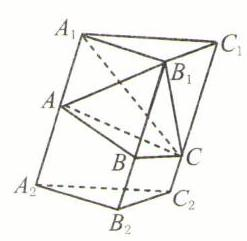
\includegraphics[width=0.2\textwidth]{bodyxb/src/bo_d20aucref24c73anc48g_211_1172_355_247_241_0.jpg}
\end{center}


(图 45)

$V = {V}_{C - A{B}_{1}B} + {V}_{C - {A}_{1}{B}_{1}A} + {V}_{C - {A}_{1}{B}_{1}{C}_{1}}.$

$\because A{A}_{1}//B{B}_{1}//C{C}_{1}$ ,且 $A{A}_{1},B{B}_{1},C{C}_{1}$ 均垂直于平面 ${ABC}$ .

$\therefore {V}_{C - A{B}_{1}B} = {V}_{{B}_{1} - {ABC}} = \dfrac{1}{3}S{h}_{2},{V}_{C - {A}_{1}{B}_{1}A} = {V}_{C - {A}_{1}{BA}} = {V}_{{A}_{1} - {ABC}} = \dfrac{1}{3}S{h}_{1}$ ,

${V}_{C - {A}_{1}{B}_{1}{C}_{1}} = {V}_{{A}_{1} - {B}_{1}C{C}_{1}} = {V}_{A - {BC}{C}_{1}} = {V}_{{C}_{1} - {ABC}} = \dfrac{1}{3}S{h}_{3}.$

$\therefore V = \dfrac{1}{3}S{h}_{2} + \dfrac{1}{3}S{h}_{1} + \dfrac{1}{3}S{h}_{3} = \dfrac{1}{3}S\left( {{h}_{1} + {h}_{2} + {h}_{3}}\right)$ .

例 8 在三棱锥 $P - {ABC}$ 中, ${MN}$ 是侧棱 ${PA}$ 和 ${BC}$ 的公垂线段,且 ${MN} = l,{PA} = a,{BC}$  $= b,{PA}$ 和 ${BC}$ 成 $\theta$ 角 (如图 46),求证: 三棱锥 $P - {ABC}$ 的体积 $= \dfrac{1}{6}{abl}\sin \theta$ .

证明 将 $\bigtriangleup {ABC}$ 补成 $▱{ABCD}$ ,连接 ${PD}$ ,则 ${PA},{AD}$ 的夹角为 $\theta$ ,且 ${BC}//$ 平面 ${PAD}$ ,故点 $C$ 到平面 ${PAD}$ 的距离即为 ${BC}$ 和平面 ${PAD}$ 的距离. $\because {MN} \bot  {PA},{MN} \bot  {BC},{BC}//{AD}$ ,

\begin{center}
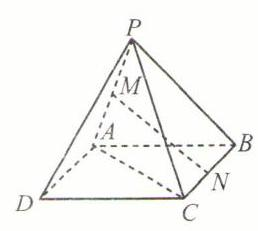
\includegraphics[width=0.2\textwidth]{bodyxb/src/bo_d20aucref24c73anc48g_211_1161_1028_258_231_0.jpg}
\end{center}


(图 46)

$\therefore {MN} \bot  {AD}$ ,于是 ${MN} \bot$ 平面 ${PAD}$ .

故 ${V}_{P - {ABC}} = {V}_{P - {ADC}} = {V}_{C - {PAD}} = \dfrac{1}{3}{S}_{\bigtriangleup {PAD}} \cdot  {MN}$

$= \dfrac{1}{3}\left( {\dfrac{1}{2} \cdot  {PA} \cdot  {AD} \cdot  \sin \theta }\right)  \cdot  {MN} = \dfrac{1}{6}{abl}\sin \theta .$

注意 当给出的几何体 (通常是三棱锥) 的体积难以直接求出时,可利用体积互等的技巧进行转换, 以达到求体积的目的.

本例也可将三棱锥补成三棱柱而获证.

\section*{【训练题】}

\section*{(A)}

175. 若底面积相等的圆锥与圆柱的体积之比为 $2 : 1$ ,则它们的高之比是(   )

(A) $2 : 1$ . (B) $4 : 1$ . (C) $6 : 1$ . (D) $8 : 1$ .

176. 已知 $E,F$ 分别是正方形 ${MNPQ}$ 的边 ${NP},{PQ}$ 的中点,沿 ${ME},{MF},{EF}$ 折成一个四面体,使 $N,P,Q$ 三点重合. 若正方形的边长为 1,则这个四面体的体积是 (   )

(A) $\dfrac{1}{24}$ . (B) $\dfrac{\sqrt{5}}{48}$ . (C) $\dfrac{\sqrt{2}}{24}$ . (D) $\dfrac{1}{8}$ .

177. 一个圆锥的高增加 10\%, 底面面积减少 10\%, 所得的圆锥体积是原圆锥体积的(   )

(A) $\dfrac{100}{99}$ . (B) $\dfrac{99}{100}$ .

(C) $\dfrac{10}{9}$ . (D) $\dfrac{9}{10}$ .

178. 圆锥的底面积为 $P$ ,轴截面面积为 $Q$ ,则此圆锥的体积等于(   )

(A) $\dfrac{2P}{3}\sqrt{\pi Q}$ . (B) $\dfrac{P}{3}\sqrt{\pi Q}$ . (C) $\dfrac{Q}{3}\sqrt{\pi P}$ . (D) $\dfrac{2Q}{3}\sqrt{\pi P}$ .

179. 将半径为 $6\mathrm{{cm}}$ 的圆形铁片,剪去 $\dfrac{1}{6}$ 后,余下部分卷成一个圆锥的侧面,则此圆锥的体积是(   )

(A) $\dfrac{25}{3}\pi {\mathrm{{cm}}}^{3}$ . (B) $\dfrac{{25}\sqrt{11}}{3}\pi {\mathrm{{cm}}}^{3}$ .

(C) ${25}\sqrt{11}{\mathrm{{cm}}}^{3}$ . (D) ${50\pi }{\mathrm{{cm}}}^{3}$ .

180. 在三棱锥 $P - {ABC}$ 中,已知三条侧棱 ${PA},{PB},{PC}$ 两两互相垂直,且 ${PC} = 1,{PA} + {PB} =$ 4,则此三棱锥的体积的最大值是(   )

(A) $\dfrac{1}{6}$ . (B) $\dfrac{1}{3}$ . (C) $\dfrac{2}{3}$ . (D) 1 .

181. 以正四面体各面中心为顶点的新四面体体积是原正四面体体积的(   )

(A) $\dfrac{1}{27}$ . (B) $\dfrac{1}{9}$ . (C) $\dfrac{1}{3}$ . (D) $\dfrac{1}{8}$ .

182. 已知正三棱台上底面边长为 2,下底面边长为 4,侧棱与底面所成的角是 ${45}^{ \circ  }$ ,则这个正三棱台的体积等于(   )

(A) $\dfrac{14}{3}$ . (B) 14. (C) $\dfrac{28}{3}$ . (D) $\dfrac{2\sqrt{3}}{9}$ .

183. 已知正六棱台的两底面边长分别为 $a$ 和 ${2a}$ ,高为 $a$ ,则其体积是(   )

(A) $\dfrac{{31}\sqrt{3}}{2}{a}^{3}$ . (B) $\dfrac{{21}\sqrt{3}}{2}{a}^{3}$ . (C) $\dfrac{7\sqrt{3}}{2}{a}^{3}$ . (D) $3\sqrt{3}{a}^{3}$ .

184. 已知 $M,N$ 分别是正方体 ${EFGH} - {E}_{1}{F}_{1}{G}_{1}{H}_{1}$ 的棱 ${F}_{1}{G}_{1},{G}_{1}{H}_{1}$ 的中点 (如图),则截面 ${MNHF}$ 将正方体分成的两部分的体积之比是(   )

\begin{center}
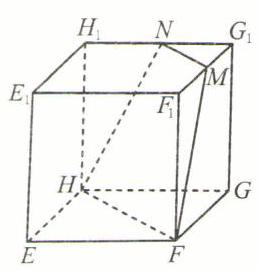
\includegraphics[width=0.2\textwidth]{bodyxb/src/bo_d20aucref24c73anc48g_212_1231_1630_258_270_0.jpg}
\end{center}


(第 184 题)

(A) $\dfrac{5}{3}$ . (B) $\dfrac{7}{5}$ .

(C) $\dfrac{9}{7}$ . (D) $\dfrac{17}{7}$ .

185. 已知正三棱台的上、下底面边长之比为 $1 : 2$ ,过上底面一边作平行于此边所对侧棱的截面将棱台分成两部分, 则这两部分的体积之比为 (   )

(A) $3 : 4$ . (B) $3 : 5$ . (C) $4 : 7$ . (D) $5 : 7$ .

186. 已知圆台的体积为 ${234}\sqrt{3}\pi {\mathrm{{cm}}}^{3}$ ,侧面展开图是半圆环,下底面半径为上底面半径的 3 倍, 则圆台的两底面半径分别是(   )

(A) $6\sqrt{3}\mathrm{{cm}}$ 和 $2\sqrt{3}\mathrm{{cm}}$ . (B) $9\mathrm{{cm}}$ 和 $3\mathrm{{cm}}$ .

(C) ${27}\mathrm{{cm}}$ 和 $9\mathrm{{cm}}$ . (D) ${18}\sqrt{3}\mathrm{{cm}}$ 和 $6\sqrt{3}\mathrm{{cm}}$ .

187. 一球内切于圆台,已知圆台的上、下底面半径分别是 $r,R$ ,则此圆台的体积是(   )

(A) $\pi \left( {{R}^{2} + {r}^{2} + {Rr}}\right) \sqrt{Rr}$ . (B) $\dfrac{2\pi }{3}\left( {{R}^{2} + {r}^{2} + {Rr}}\right) \sqrt{Rr}$ .

(C) $\dfrac{\pi }{3}\left( {{R}^{2} + {r}^{2} + {Rr}}\right) \sqrt{Rr}$ . (D) $\dfrac{\pi }{6}\left( {{R}^{2} + {r}^{2} + {Rr}}\right) \sqrt{Rr}$ .

188. (1)已知正三棱锥的高为 3,侧面与底面所成的角为 ${60}^{ \circ  }$ ,则它的全面积为\blkda{},体积为\blkda{}；

(2)已知三棱锥的三条侧棱两两互相垂直,且长度分别为 $1\mathrm{{cm}},2\mathrm{{cm}},3\mathrm{{cm}}$ ,则此棱锥的体积是\blkda{} ${\mathrm{{cm}}}^{3}$ ；

(3)已知三棱锥的三个侧面两两互相垂直,它们的面积分别是 $6{\mathrm{{cm}}}^{2},4{\mathrm{{cm}}}^{2}$ 和 $3{\mathrm{{cm}}}^{2}$ ,则它的体积为\blkda{} ${\mathrm{{cm}}}^{3}$ ；

(4)正方体的棱长为 $a$ ,以它相对两面中一对异面对角线的四个顶点作三棱锥,则这个三棱棱锥的体积为\blkda{},高为\blkda{}；

(5)将边长为 $3\mathrm{{cm}}$ , $4\mathrm{{cm}}$ 的矩形 ${ABCD}$ 沿对角线 ${BD}$ 折成直二面角,则四面体 ${ABCD}$ 的体积等于\blkda{} ${\mathrm{{cm}}}^{3}$ ；

(6)设正四棱锥底面面积为 $Q$ ,侧面面积为 $S$ ,则它的体积等于\blkda{}；

(7)过四面体一个顶点的三条棱的中点作截面,切去四面体的一个角. 用同样的方法切去其余三个角,若原四面体的体积为 $V$ ,则切去四个角后的几何体的体积等于\blkda{}.

189. (1) 圆锥的高缩小为原来的 $\dfrac{1}{2}$ ,底面半径扩大为原来的 2 倍后,则体积是原来体积的\blkda{}；

(2)若一个圆锥的侧面展开图(扇形)的圆心角为 ${90}^{ \circ  }$ ,扇形的半径是 ${12}\mathrm{{cm}}$ ,则这个圆锥的体积为\blkda{} ${\mathrm{{cm}}}^{3}$ ；

(3)若圆锥的体积为 $V$ ,轴截面面积为 $S$ ,则圆锥底面的半径长为\blkda{}；

(4)在等边三角形 ${ABC}$ 中,边长为 $a$ ,现将 $\bigtriangleup {ABC}$ 绕直线 ${AB}$ 旋转一周,所得旋转体的体积为\blkda{}.

190. (1) 已知圆台的上、下底面半径分别为 ${10}\mathrm{{cm}},{18}\mathrm{{cm}}$ ,轴截面面积为 ${420}{\mathrm{{cm}}}^{2}$ ,则此圆台的体积为\blkda{} ${\mathrm{{cm}}}^{3}$ ；

(2)已知棱台的体积为 ${76}{\mathrm{{cm}}}^{3}$ ,高 $6\mathrm{{cm}}$ ,一个底面面积为 ${18}{\mathrm{{cm}}}^{2}$ ,则另一个底面面积为\blkda{} ${\mathrm{{cm}}}^{2}$ ；

(3)已知正四棱台的上、下底面边长分别是 $2\mathrm{{cm}}$ 和 $4\mathrm{{cm}}$ ,侧棱与底面成 ${45}^{ \circ  }$ ,则其体积为\blkda{} ${\mathrm{{cm}}}^{3}$ ；

(4)已知棱台高 $h$ 为 20,体积 $V$ 为 1720,两底面边长之比为 $5 : 8$ ,则上、下底面面积分别等于\blkda{}；

(5)已知正四棱台 ${ABCD} - {A}_{1}{B}_{1}{C}_{1}{D}_{1}$ 的上、下底面边长分别为 $a$ 与 ${2a}$ ,过上底面对角线 ${A}_{1}{C}_{1}$ 与下底面顶点 $B$ 作截面,截得小棱锥 ${B}_{1} - {A}_{1}B{C}_{1}$ . 记原正四棱台的体积为 $V$ ,则截得的小棱锥的体积等于\blkda{}.

191. (1) 已知圆锥的高与母线的夹角为 ${30}^{ \circ  }$ ,底面圆中长为 $4\mathrm{{cm}}$ 的弦所对的圆心角为 ${60}^{ \circ  }$ ,求这个圆锥的体积;

(2)一个倒放的圆锥形封闭容器,高为 ${2h}$ ,装入水,使水高为圆锥高的 $\dfrac{1}{2}$ ,则倒转容器后, 水的高度是多少?

192. (1) 已知 $E,F$ 分别是棱长为 $a$ 的正四面体 ${ABCD}$ 的棱 ${AB},{CD}$ 的中点,将 $\bigtriangleup {AEF}$ 绕直线 ${AF}$ 旋转一周,求所得旋转体的体积；

\begin{center}
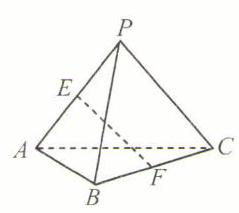
\includegraphics[width=0.2\textwidth]{bodyxb/src/bo_d20aucref24c73anc48g_214_1270_754_239_213_0.jpg}
\end{center}


[第 192(3)题]

(2)在四面体 $O - {ABC}$ 中,除 ${OC}$ 外其余的棱长均为 1 ,且 ${OC}$ 与平面 ${ABC}$ 所成角的余弦值为 $\dfrac{1}{3}$ ,求此四面体的体积;

(3)在三棱锥 $P - {ABC}$ 中,已知 ${PA}\bot {BC},{PA} = {BC} = a,{PA},{BC}$ 的公垂线段为 ${EF}$ ,且 ${EF} = h$ (如图),求三棱锥 $P - {ABC}$ 的体积.

193. (1) 已知等边圆柱的轴截面 ${ABCD}$ 的面积为 4,点 $Q$ 在下底面的圆周上移动,当四面体 $A - {BQC}$ 的体积最大时,求点 $C$ 到平面 ${ABQ}$ 的距离;

(2)已知圆锥的全面积为 $\pi$ ,求圆锥的体积的最大值.

\section*{(B)}

194. 平行四边形两邻边长分别为 $a$ 和 $b$ ,则当它们分别绕边 $a$ 和 $b$ 旋转一周,所成的两个几何体的体积之比为 (   )

(A) 1 . (B) $\dfrac{b}{a}$ . (C) $\dfrac{{b}^{2}}{{a}^{2}}$ . (D) $\dfrac{{b}^{3}}{{a}^{3}}$ .

195. 若圆锥被平行于底面的平面截成侧面积相等的两部分, 且小圆锥的体积为 1 , 则原圆锥的体积是(   )

(A) $\sqrt{2}$ . (B) $2\sqrt{2}$ . (C) 9. (D) 12.

196. 若平行六面体 ${ABCD} - {A}_{1}{B}_{1}{C}_{1}{D}_{1}$ 的体积为 30,则三棱锥 ${B}_{1} - A{D}_{1}C$ 的体积等于(   )

(A) 6. (B) 7.5. (C) 10. (D) 15.

197. 在平行六面体交于一点 $A$ 的三条棱上分别取中点 $E,F,G$ ,则棱锥 $A - {EFG}$ 的体积是平行六面体体积的(   )

(A) $\dfrac{1}{8}$ . (B) $\dfrac{1}{16}$ . (C) $\dfrac{1}{24}$ . (D) $\dfrac{1}{48}$ .

198. 在三棱锥 $P - {ABC}$ 的三条侧棱 ${PA},{PB},{PC}$ 上分别取点 $E,F,G$ ,使 ${PE} = \dfrac{1}{2}{PA},{PF} =$  $\dfrac{1}{3}{PB},{PG} = \dfrac{3}{4}{PC}$ ,若三棱锥 $P - {EFG}$ 的体积等于 1,则多面体 ${EFG} - {ABC}$ 的体积为(   )

(A) 3 . (B) 5. (C) 7. (D) 8.

199. 已知三角形的三边长分别为 $a,b,c$ ,分别以各边所在直线为轴将三角形旋转一周,得到的三个旋转体的体积之比为(   )

(A) $a : b : c$ . (B) ${a}^{3} : {b}^{3} : {c}^{3}$ . (C) $\dfrac{1}{a} : \dfrac{1}{b} : \dfrac{1}{c}$ . (D) $\dfrac{1}{{a}^{3}} : \dfrac{1}{{b}^{3}} : \dfrac{1}{{c}^{3}}$ .

200. 若 $P$ 是棱长为 1 的正四面体内的任意一点,则它到这个四面体各面的距离之和为 (   )

(A) $\dfrac{\sqrt{3}}{2}$ . (B) $\dfrac{\sqrt{3}}{3}$ . (C) $\dfrac{\sqrt{6}}{2}$ . (D) $\dfrac{\sqrt{6}}{3}$ .

201. 已知两个平行于底面的平面将圆锥的高分成相等的三段,则此圆锥所分成的三部分的体积(自上至下)之比为(   )

(A) $1 : 2 : 3$ . (B) $1 : 4 : 9$ . (C) $1 : 8 : {27}$ . (D) $1 : 7 : {19}$ .

202. (1)已知三棱锥 $P - {ABC}$ 的三条侧棱两两互相垂直, ${PA} = 5,{PB} = 4,{PC} = 3,D$ 为 ${AB}$ 的中点, $E$ 为 ${AC}$ 的中点,则四棱锥 $P - {BCED}$ 的体积是\blkda{} ${\mathrm{{cm}}}^{3}$ ；

(2)在三棱锥 $P - {ABC}$ 中,除棱 ${PA}$ 外,其余各棱长均为 $a\mathrm{{cm}}$ ,则当棱 ${PA}$ 长为\blkda{} 时,此三棱锥的体积有最大值等于\blkda{} ${\mathrm{{cm}}}^{3}$ .

203. 在单位正方体 ${ABCD} - {A}_{1}{B}_{1}{C}_{1}{D}_{1}$ 中 (如图),

(1)若 $E$ 是棱 ${CD}$ 的中点,求点 ${D}_{1}$ 到平面 ${AE}{C}_{1}$ 的距离；

(2)若 $E$ , $F$ 分别是棱 ${CD}$ 和 $D{D}_{1}$ 的中点,求点 $E$ 到平面 ${A}_{1}{C}_{1}F$ 的距离.

\begin{center}
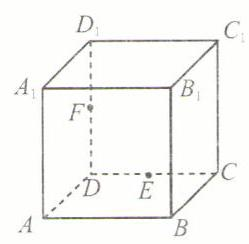
\includegraphics[width=0.2\textwidth]{bodyxb/src/bo_d20aucref24c73anc48g_215_379_1408_249_244_0.jpg}
\end{center}


(第 203 题)

\begin{center}
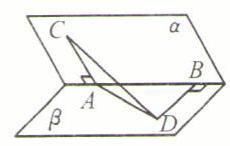
\includegraphics[width=0.2\textwidth]{bodyxb/src/bo_d20aucref24c73anc48g_215_879_1504_230_146_0.jpg}
\end{center}


(第 204 题)

204. 已知 $A,B$ 为二面角 $\alpha  - {AB} - \beta$ 棱上两点,点 $C \in  \alpha$ ,点 $D \in  \beta$ ,且 ${AC} \bot  {AB},{BD} \bot  {AB},{AB}$  $= 4\mathrm{{cm}},{AC} = 6\mathrm{{cm}},{BD} = 8\mathrm{{cm}},{CD} = 2\sqrt{17}\mathrm{{cm}}$ (如图),求:

(1)二面角 $\alpha  - {AB} - \beta$ 的大小； (2)点 $B$ 到平面 ${CAD}$ 的距离.

205. 已知三棱锥 $P - {ABC}$ 的侧棱 ${PA} \bot$ 底面 ${ABC}$ ,且底面是 $\angle {ACB} =$  ${90}^{ \circ  }$ 的直角三角形,过点 $A$ 的截面与 ${PB}$ 垂直,垂足为 $D$ ,该平面与 ${PC}$ 交于点 $E$ (如图).

\begin{center}
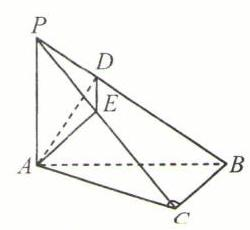
\includegraphics[width=0.2\textwidth]{bodyxb/src/bo_d20aucref24c73anc48g_215_1159_1931_250_230_0.jpg}
\end{center}


(第 205 题)

(1)求证: ${AE}\bot {DE}$ ；

(2)若 ${PA} = {AC} = {BC} = a$ ,求三棱锥 $P - {ADE}$ 的体积.

206. 在四边形 ${ABCD}$ 中,已知 $\angle {BAD} = {120}^{ \circ  },\angle {BCD} = {60}^{ \circ  },{AB} = {AD} = 1,{BC} = {CD}$ ,且 $E,F$ 分别是 ${BC},{CD}$ 的中点 (如图甲). 今沿折线 ${AE},{EF},{FA}$ 折起,使 $B,C,D$ 三点重合于一点 $M$ (如图乙),求四面体 ${AMEF}$ 的体积.

\begin{center}
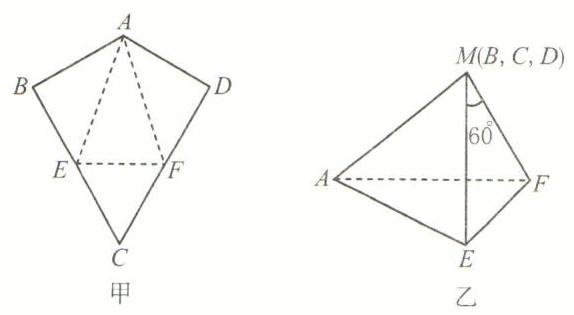
\includegraphics[width=0.4\textwidth]{bodyxb/src/bo_d20aucref24c73anc48g_216_570_322_574_315_0.jpg}
\end{center}


(第 206 题)

207. 用边长为 $9\mathrm{{cm}}$ 的正方形 ${AD}{D}_{1}{A}_{1}$ 纸片 (如图甲) 折成一个正三棱柱的侧面,此时原正方形的对角线 $A{D}_{1}$ 被折成一条空间折线 ${APQ}{A}_{1}$ (如图乙). 求:

(1)异面直线 ${AP}$ 与 ${A}_{1}Q$ 所成角的余弦值； (2)四面体 $A - {PQ}{A}_{1}$ 的体积.

\begin{center}
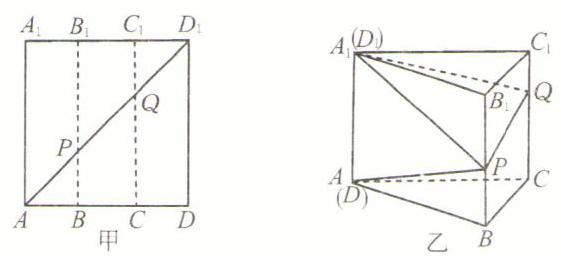
\includegraphics[width=0.4\textwidth]{bodyxb/src/bo_d20aucref24c73anc48g_216_577_882_561_256_0.jpg}
\end{center}


(第 207 题)

208. 已知斜三棱柱 ${ABC} - {A}_{1}{B}_{1}{C}_{1}$ 的底面 $\bigtriangleup  {ABC}$ 是直角三角形, $\angle {ACB} = {90}^{ \circ  }$ ,侧棱与平面 ${ABC}$ 成 ${60}^{ \circ  }$ 角,点 ${B}_{1}$ 在平面 ${ABC}$ 上的射影 $D$ 为 ${BC}$ 的中点 (如图).

\begin{center}
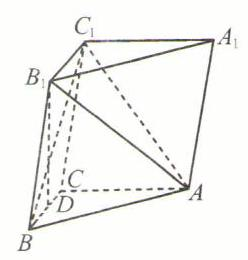
\includegraphics[width=0.2\textwidth]{bodyxb/src/bo_d20aucref24c73anc48g_216_1270_1214_248_260_0.jpg}
\end{center}


(第 208 题)

(1)求证: $A{B}_{1}\bot B{C}_{1}$ ；

(2)若侧面 ${A}_{1}{AB}{B}_{1}$ 与侧面 ${C}_{1}{CB}{B}_{1}$ 成 ${30}^{ \circ  }$ 的二面角,且 ${BC} =$  $2\mathrm{{cm}}$ ,求四棱锥 $A - {B}_{1}{BC}{C}_{1}$ 的体积.

209. 已知圆柱的两底面中心为 $O,{O}_{1}$ ,底面半径为 $R$ ,高为 $h$ ,上底面半径 ${OA}$ 所在直线与下底面半径 ${O}_{1}B$ 所在直线成 $\theta$ 角 $\left( {0 < \theta  < \dfrac{\pi }{2}}\right)$ . 求:

(1) $O{O}_{1}$ 与 ${AB}$ 所成角的正切值；(2)以 $O,{O}_{1},A,B$ 为顶点的四面体的体积.

210. 斜三棱柱 ${ABC} - {A}^{\prime }{B}^{\prime }{C}^{\prime }$ 的每条棱长都为 $a$ ,侧棱与底面所成的角等于 ${60}^{ \circ  }$ ,且侧面 ${BC}{C}^{\prime }{B}^{\prime }$ 垂直于底面 ${ABC}$ (如图, $\angle {C}^{\prime }{CB}$ 为锐角).

\begin{center}
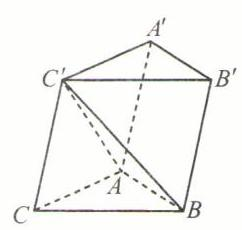
\includegraphics[width=0.2\textwidth]{bodyxb/src/bo_d20aucref24c73anc48g_216_1267_1757_242_230_0.jpg}
\end{center}


(第 210 题)

(1)求证: ${C}^{\prime }A \bot  {BC}$ ；

(2)求四棱锥 ${C}^{\prime } - {AB}{B}^{\prime }{A}^{\prime }$ 的体积.

211. (1) 已知 ${ABCD} - {A}_{1}{B}_{1}{C}_{1}{D}_{1}$ 是棱长为 $a$ 的正方体, $E$ , $F$ 分别为棱 $A{A}_{1}$ 与 $C{C}_{1}$ 的中点 (如图),求四棱锥 ${A}_{1} - {EBF}{D}_{1}$ 的体积;

(2)已知直三棱柱 ${ABC} - {A}^{\prime }{B}^{\prime }{C}^{\prime }$ 的体积为 $V,P,Q$ 分别是侧棱 $A{A}^{\prime },C{C}^{\prime }$ 上的点,且 ${AP}$  $= {C}^{\prime }Q$ (如图),求四棱锥 $B - {APQC}$ 的体积;

(3)已知 $E$ , $F$ 分别是正方体 ${ABCD} - {A}_{1}{B}_{1}{C}_{1}{D}_{1}$ 棱 ${BC}$ , $D{D}_{1}$ 的中点(如图),若正方体的棱长为 1,求四面体 $A - {B}_{1}{EF}$ 的体积.

\begin{center}
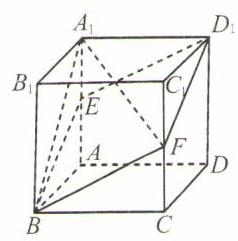
\includegraphics[width=0.2\textwidth]{bodyxb/src/bo_d20aucref24c73anc48g_217_245_351_238_241_0.jpg}
\end{center}


[第 211(1)题]

\begin{center}
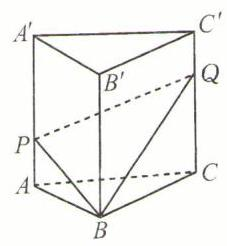
\includegraphics[width=0.2\textwidth]{bodyxb/src/bo_d20aucref24c73anc48g_217_614_343_227_246_0.jpg}
\end{center}


[第 211(2)题]

\begin{center}
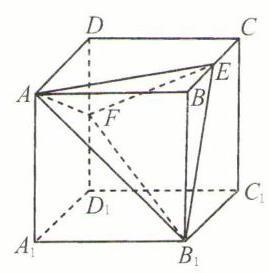
\includegraphics[width=0.2\textwidth]{bodyxb/src/bo_d20aucref24c73anc48g_217_973_311_269_273_0.jpg}
\end{center}


[第 211(3)题]

212. 正方体 ${ABCD} - {A}_{1}{B}_{1}{C}_{1}{D}_{1}$ 的棱长为 $a,{EF}$ 是棱 ${AB}$ 上的一条长度为 $b\left( {b < a}\right)$ 的可滑动线段, $P,Q$ 分别是棱 ${A}_{1}{D}_{1},{D}_{1}{C}_{1}$ 上的两个动点 (如图),求以 $E,F,P,Q$ 为顶点的四面体体积的最大值.

\begin{center}
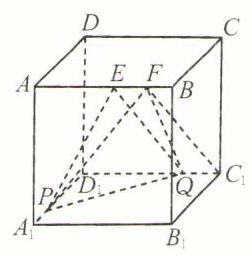
\includegraphics[width=0.2\textwidth]{bodyxb/src/bo_d20aucref24c73anc48g_217_186_831_252_256_0.jpg}
\end{center}


(第 212 题)

\begin{center}
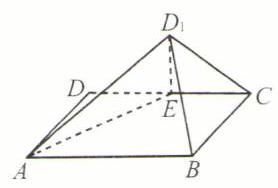
\includegraphics[width=0.2\textwidth]{bodyxb/src/bo_d20aucref24c73anc48g_217_600_898_278_188_0.jpg}
\end{center}


(第 213 题)

\begin{center}
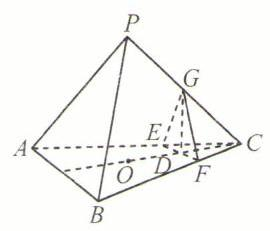
\includegraphics[width=0.2\textwidth]{bodyxb/src/bo_d20aucref24c73anc48g_217_1040_849_270_231_0.jpg}
\end{center}


(第 214 题)

213. 已知矩形 ${ABCD},E$ 为 ${CD}$ 的中点,沿 ${AE}$ 将矩形折成二面角 ${D}_{1} - {AE} - B$ (如图), ${AB} =$  $2,{BC} = 1,B{D}_{1} = C{D}_{1}$ .

(1)求证:平面 $A{D}_{1}E \bot$ 平面 ${ABC}$ ；

(2)求二面角 ${D}_{1} - {AB} - E$ 的正切值；

(3)求三棱锥 ${D}_{1} - {ABE}$ 的体积.

214. 正三棱锥 $P - {ABC}$ 的底面中心是 $O,D$ 是 ${OC}$ 的中点,过点 $D$ 作截面 ${EFG}$ 与 ${OC}$ 垂直 (如图),求该截面将棱锥分成的两部分的体积之比.

\begin{center}
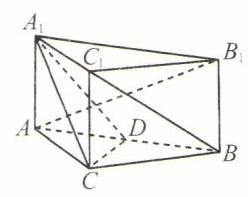
\includegraphics[width=0.2\textwidth]{bodyxb/src/bo_d20aucref24c73anc48g_217_1177_1433_248_197_0.jpg}
\end{center}


(第 215 题)

215. 在斜三棱柱 ${ABC} - {A}_{1}{B}_{1}{C}_{1}$ 中,已知 ${AC} = {BC},D$ 为 ${AB}$ 的中点,平面 ${A}_{1}{B}_{1}{C}_{1} \bot$ 平面 ${AB}{B}_{1}{A}_{1}$ ,且异面直线 $B{C}_{1}$ 与 $A{B}_{1}$ 互相垂直 (如图).

(1)求证: $A{B}_{1}\bot$ 平面 ${A}_{1}{CD}$ ；

(2)若 $C{C}_{1}$ 与平面 ${AB}{B}_{1}{A}_{1}$ 的距离为 $1,{A}_{1}C = \sqrt{37},A{B}_{1} = 5$ ,求三棱锥 ${A}_{1} - {ACD}$ 的体积.

\section*{(三) 球的体积}

\section*{【典型题型和解题技巧】}

正如三角形的内切圆半径常常与面积发生联系一样, 多面体的内切球半径常常和体积发生联系.

例 如图 47,三棱锥 $A - {BCD}$ 的两条棱 ${AB} - {CD} - 6$ ,其余各棱长均为 5,求该三棱锥的内切球半径.

解 取 ${CD}$ 的中点 $E$ ,连接 ${AE}$ , ${BE}$ ,由 ${CD} \bot  {AE}$ , ${CD} \bot  {BE}$ ,得 ${CD}$  $\bot$ 平面 ${ABE}$ .

\begin{center}
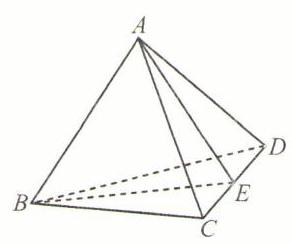
\includegraphics[width=0.2\textwidth]{bodyxb/src/bo_d20aucref24c73anc48g_218_1235_211_292_244_0.jpg}
\end{center}


(图 47)

由 ${AD} = 5,{DE} = 3$ ,得 ${AE} = {BE} = 4$ ,故 $\bigtriangleup {ABE}$ 的面积 $= 3\sqrt{7}$ . 于是 ${V}_{A - {BCD}} = {V}_{C - {ABE}} + {V}_{D - {ABE}} = \dfrac{1}{3}{S}_{\bigtriangleup {ABE}} \cdot  {CD} = \dfrac{1}{3} \cdot  3\sqrt{7} \cdot  6 = 6\sqrt{7}.$

显然, 三棱锥的四个侧面全等, 各侧面的面积为 12 .

设三棱锥的内切球半径为 $r$ ,

则 ${V}_{A - {BCD}} = \dfrac{1}{3}\left( {{S}_{\bigtriangleup {ABC}} + {S}_{\bigtriangleup {BCD}} + {S}_{\bigtriangleup {CDA}} + {S}_{\bigtriangleup {DAB}}}\right)  \cdot  r = \dfrac{1}{3} \cdot  {48r} = {16r}$ ,

由此便得内切球半径 $r = \dfrac{3\sqrt{7}}{8}$ .

\section*{【训练题】}

\section*{(A)}

216. 若一个球的外切正方体的全面积等于 $6{\mathrm{{cm}}}^{2}$ ,则此球的体积等于 (   )

(A) $\dfrac{4}{3}\pi {\mathrm{{cm}}}^{3}$ . (B) $\dfrac{\sqrt{6}}{6}\pi {\mathrm{{cm}}}^{3}$ . (C) $\dfrac{\sqrt{6}\pi }{8}{\mathrm{{cm}}}^{3}$ . (D) $\dfrac{\pi }{6}{\mathrm{{cm}}}^{3}$ .

217. 已知等边圆柱的侧面积与一个球的表面积相等, 则这个圆柱与这个球的体积之比是(   )

(A) $1 : 1$ . (B) $3 : 4$ . (C) $4 : 3$ . (D) $3 : 2$ .

218. 一个球与它的外切圆柱、外切等边圆锥的体积之比为(   )

(A) $2 : 3 : 5$ . (B) $2 : 3 : 4$ . (C) $3 : 5 : 8$ . (D) $4 : 6 : 9$ .

219. 若一个圆柱和一个圆锥的底面直径和高都与球的直径相等,则其体积之比 ${V}_{\text{ 圆柱 }} : {V}_{\text{ 球 }}$ : ${V}_{\text{ 圆锥 }}$ 为(   )

(A) $3 : 2 : 1$ . (B) $3 : 4 : 1$ . (C) $6 : 4 : \sqrt{3}$ . (D) $1 : 2 : 3$ .

220. 表面积相等的球及正方体的体积依次记为 ${V}_{\text{ 球 }}$ 和 ${V}_{\text{ 正方体 }}$ ,球的直径为 $d$ ,正方体的棱长为 $a$ ,则(   )

(A) $d > a,{V}_{\text{ 球 }} > {V}_{\text{ 正方体 }}$ . (B) $d > a,{V}_{\text{ 球 }} < {V}_{\text{ 正方体 }}$ .

(C) $d < a,{V}_{\text{ 球 }} > {V}_{\text{ 正方体 }}$ . (D) $d < a,{V}_{\text{ 球 }} < {V}_{\text{ 正方体 }}$ .

221. 若球的大圆面积扩大为原来的 3 倍,则它的体积扩大为原来的(   )

(A) 3 倍. (B) 27 倍. (C) $3\sqrt{3}$ 倍. (D) $\sqrt[3]{3}$ 倍.

222. 若球面积扩大为原来的 9 倍, 则球的体积扩大为原来的 (   )

(A) 3 倍. (B) 9 倍.

(C) 27 倍. (D) 81 倍.

223. 已知扇形 ${AOB}$ 的圆心角为 ${90}^{ \circ  },\overset{⏜}{AB}$ 所对的弦 ${AB}$ 将扇形分成两个部分 (如图),这两部分各以 ${AO}$ 为轴旋转一周,所得两部分旋转体的体积之比为(   )

\begin{center}
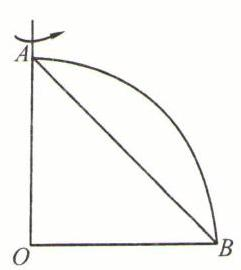
\includegraphics[width=0.2\textwidth]{bodyxb/src/bo_d20aucref24c73anc48g_219_1175_145_241_270_0.jpg}
\end{center}


(第 223 题)

(A) $1 : 1$ . (B) $1 : \sqrt{2}$ .

(C) $2 : 1$ . (D) $\left( {\pi  - 2}\right)  : 2$ .

224. 已知高与底面直径之比为 $2 : 1$ 的圆柱内接于球,且圆柱的体积等于 ${500\pi }{\mathrm{{cm}}}^{3}$ ,则球的体积为(   )

(A) $\dfrac{500}{3}\pi {\mathrm{{cm}}}^{3}$ . (B) $\dfrac{2500}{3}\pi {\mathrm{{cm}}}^{3}$ .

(C) $\dfrac{2500}{3}\sqrt{5}\pi {\mathrm{{cm}}}^{3}$ . (D) $\dfrac{12500}{3}\pi {\mathrm{{cm}}}^{3}$ .

225. (1)表面积为 $S$ 的球的体积等于\blkda{}；

(2)若一个球的表面积等于一个轴截面为正方形的圆柱的侧面积,则这个球的体积与这个圆柱的体积之比等于\blkda{}；

(3) 三个大小不等的球,若它们的表面积之比是 $1 : 2 : 3$ ,则它们的体积之比是\blkda{}.

226. (1)若球的外切圆台的上、下底面半径分别为 1 和 3 ,则球的体积为\blkda{}；

(2)若正三棱柱有一个半径为 $\sqrt{3}\mathrm{{cm}}$ 的内切球,则此棱柱的体积是\blkda{} ${\mathrm{{cm}}}^{3}$ ,全面积是\blkda{} $\mathrm{{cm}}$ ；

(3)已知圆锥的高与其外接球半径之比为 $q$ ,则圆锥体积与球体积之比为\blkda{}；

(4)已知一个球内切于上、下底面边长分别为 $a,b\left( {a < b}\right)$ 的正四棱台,则这个棱台的体积是\blkda{}；

(5)已知球的体积为 $V$ ,在它里面有一个轴截面顶角为 $\theta$ 的内接圆锥,则圆锥的体积为\blkda{}.

\section*{(B)}

227. 已知两球的体积之和是 ${12\pi }$ ,且两球的大圆周长之和是 ${6\pi }$ ,则两球的半径之差等于(   )

(A) 1 . (B) 2 . (C) 3. (D) 4.

228. 正四面体的内切球球心到一个面的距离等于这个正四面体高的(   )

(A) $\dfrac{1}{2}$ . (B) $\dfrac{1}{3}$ . (C) $\dfrac{1}{4}$ . (D) $\dfrac{1}{5}$ .

229. (1)半径为 $R$ 的球的内接正方体体积是\blkda{}；

(2)在球面上有四个点 $P,A,B,C$ ,若 ${PA} = {PB} = {PC} = a$ ,且 ${PA},{PB},{PC}$ 两两互相垂直,则这个球的体积是\blkda{}；

(3)一个长方体同一顶点的三个面的对角线分别是 $a,b,c$ ,则它的外接球体积为\blkda{}.

* 230. (1) 已知球的半径为 5 , 用两个平行平面去截球, 截面半径分别为 3 与 4 , 则夹在这两个平行截面间的球体部分的体积为\blkda{}；

(2)一个球缺的高是其底面半径的 $\dfrac{1}{3}$ ,则球缺体积与整个球体积之比为\blkda{}.

231. (1) 若球的半径为 $r$ ,求其内接正四面体的体积；

(2)若三棱锥的全面积为 $S$ ,体积为 $V$ ,求它的内切球的体积.

232. (1) 已知正四棱台的上、下底面边长之比为 $m : n$ ,求棱台与其内切球的体积之比;

(2)圆台外切于球,且圆台的侧面积与此球的表面积之比为 $4 : 3$ ,求圆台的体积与球的体积之比.

233. (1) 已知圆锥的高与其外接球半径的比为 $q$ ,求圆锥与球的表面积之比;

(2)求证:球与它的外切圆锥的体积之比等于它们相应的表面积之比.

\section*{(C)}

234. $P$ 是棱长为 1 的正方体 ${ABCD} - {A}_{1}{B}_{1}{C}_{1}{D}_{1}$ 的棱 ${A}_{1}{B}_{1}$ 上的动点,过点 $P,B,{D}_{1}$ 作截面 (如图), 求截面面积的最小值.

\begin{center}
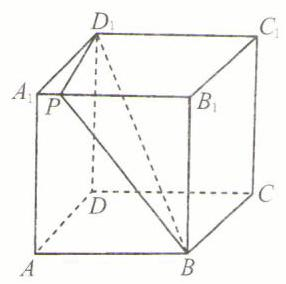
\includegraphics[width=0.2\textwidth]{bodyxb/src/bo_d20aucref24c73anc48g_220_321_982_286_284_0.jpg}
\end{center}


(第 234 题)

\begin{center}
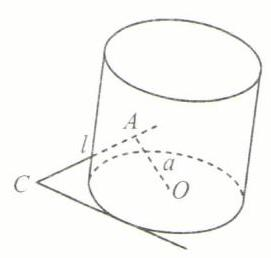
\includegraphics[width=0.2\textwidth]{bodyxb/src/bo_d20aucref24c73anc48g_220_742_1009_271_258_0.jpg}
\end{center}


(第 235 题)

\begin{center}
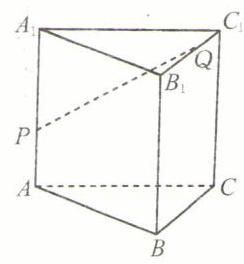
\includegraphics[width=0.2\textwidth]{bodyxb/src/bo_d20aucref24c73anc48g_220_1130_1002_244_264_0.jpg}
\end{center}


(第 237 题)

235. 直线 $l$ 切圆柱侧面于点 $A$ ,并与圆柱底面成 $\alpha$ 角 (如图),已知圆柱底面圆心 $O$ 与点 $A$ 的距离为 $a$ ,底面半径为 $b$ ,求点 $O$ 到直线 $l$ 的距离.

236. 从空间一点 $O$ 出发引四条射线,其中任意两条射线之间的夹角相等,求夹角的余弦值.

237. 在正三棱柱 ${ABC} - {A}_{1}{B}_{1}{C}_{1}$ 中,已知 ${A}_{1}A = 3,P,Q$ 分别是棱 ${A}_{1}A,{B}_{1}{C}_{1}$ 上的点, ${AP} =$  $1,{PQ}$ 与平面 ${A}_{1}{AB}{B}_{1},{B}_{1}{BC}{C}_{1}$ 都成 ${30}^{ \circ  }$ 角 (如图),求该三棱柱的体积.

238. 已知四面体的三组对棱分别等长,根据下列条件,求它的体积:

(1)三组对棱长分别为4,5,6；

(2)三组对棱长分别为 $a,b,c$ .

\begin{center}
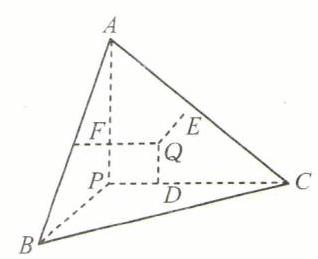
\includegraphics[width=0.2\textwidth]{bodyxb/src/bo_d20aucref24c73anc48g_220_1177_1751_318_259_0.jpg}
\end{center}


(第 239 题)

239. 三棱锥 $P - {ABC}$ 的侧棱 ${PA},{PB},{PC}$ 两两互相垂直,长分别为 $a,b,c$ (如图),试用“体积法”证明:

(1)若点 $P$ 到底面 ${ABC}$ 的距离为 $h$ ,则 $\dfrac{1}{{h}^{2}} = \dfrac{1}{{a}^{2}} + \dfrac{1}{{b}^{2}} + \dfrac{1}{{c}^{2}}$ ；

(2)若 $Q$ 为底面 ${ABC}$ 上任意一点,点 $Q$ 到三个侧面的距离 ${QD},{QE},{QF}$ 分别为 $x,y,z$ ,则 $\dfrac{x}{a} + \dfrac{y}{b} + \dfrac{z}{c} = 1$ .

240. 四面体 ${ABCD}$ 各顶点到对面的距离分别为 $a,b,c,d$ ,四面体体内一点 $P$ 到面 ${BCD}$ ,面 ${CDA}$ ,面 ${DAB}$ ,面 ${ABC}$ 的距离依次为 ${a}_{1},{b}_{1},{c}_{1},{d}_{1}$ ,求证: $\dfrac{{a}_{1}}{a} + \dfrac{{b}_{1}}{b} + \dfrac{{c}_{1}}{c} + \dfrac{{d}_{1}}{d} = 1$ .

241. 在四面体 ${ABCD}$ 中, $E,F$ 分别是相对棱 ${AB},{CD}$ 的中点,过 $E,F$ 作截面交对棱 ${BC},{AD}$ (或其延长线) 于点 $H,M$ (如图). 求证: ${HM}$ 被 ${EF}$ 所平分.

\begin{center}
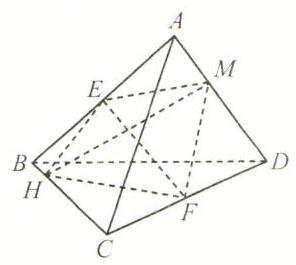
\includegraphics[width=0.2\textwidth]{bodyxb/src/bo_d20aucref24c73anc48g_221_213_378_296_265_0.jpg}
\end{center}


(第 241 题)

\begin{center}
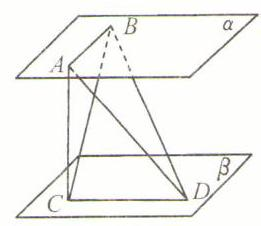
\includegraphics[width=0.2\textwidth]{bodyxb/src/bo_d20aucref24c73anc48g_221_667_414_261_226_0.jpg}
\end{center}


(第 242 题)

\begin{center}
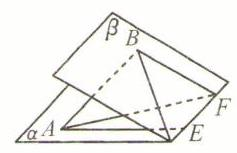
\includegraphics[width=0.2\textwidth]{bodyxb/src/bo_d20aucref24c73anc48g_221_1092_479_237_153_0.jpg}
\end{center}


(第 243 题)

242. ${AB},{CD}$ 是两平行平面 $\alpha ,\beta$ 内互相垂直的两条线段,若 ${AB} = {CD} = a,\alpha ,\beta$ 间的距离为 $h$ (如图),求四面体 ${ABCD}$ 的体积;

243. $E,F$ 分别是 ${30}^{ \circ  }$ 的二面角 $\alpha  - {EF} - \beta$ 的棱上的两个定点, ${EF} = a$ ,过点 $E,F$ 分别在 $\alpha ,\beta$ 内作棱 ${EF}$ 的垂线, $A,B$ 分别是两条垂线上的动点,且满足 ${AB} = \sqrt{2}a$ (如图),求四面体 ${ABEF}$ 的体积的最大值.

244. 分别以 $\bigtriangleup {ABC}$ 的边 ${BC},{CA},{AB}$ 为轴,把三角形旋转一周,所得的几何体体积分别为 ${V}_{1},{V}_{2},{V}_{3}.P$ 为 $\bigtriangleup  {ABC}$ 内一点,且到 ${BC},{CA},{AB}$ 的距离之比为 ${V}_{1} : {V}_{2} : {V}_{3}$ ,则 $P$ 是 $\bigtriangleup {ABC}$ 的什么点?

245. 在三棱锥 $P - {ABC}$ 中,已知 ${PA} \bot$ 底面 ${ABC},\angle {ABC} = {90}^{ \circ  }$ ,求这个三棱锥的外接球球心的位置.

246. 四棱锥 $P - {ABCD}$ 的底面为矩形,侧面 ${PAD}$ 为等边三角形,侧面 ${PAD} \bot$ 底面 ${ABCD}$ ,若 ${PD} = 4\sqrt{3},{AB} = 8$ ,求这个四棱锥的内切球半径.

247. 在三棱锥 $A - {BCD}$ 中,已知 ${AB} = 4,{CD} = {12}$ ,其余各棱均为 7,求三棱锥的内切球球心 $O$ 到棱 ${CD}$ 的距离.

248. 圆柱的直径为 ${4r}$ ,高为 ${22r}$ ,此圆柱最多能装半径为 $r$ 的球多少个?

249. 已知两个正方体,一个正方体的一条棱长与另一个正方体一条棱长之和为 ${10}\mathrm{{cm}}$ ,当它们的棱长各为多少时,这两个正方体的体积之和最小？最小值是多少？

250. ${MN}$ 是异面直线 $a,b$ 的公垂线段,长度为定长的线段 ${PQ}$ 的两端分别在 $a,b$ 上滑动,其中 $M,P \in  a,N,Q \in  b$ ,且四点互不相同. 求证: 过 $M,N,P,Q$ 四点的球的半径为定值,并求这个定值.

251. 已知 ${AB}$ 是球 $O$ 的直径, $C$ , $D$ 是球面上的两点,且点 $D$ 在以 ${BC}$ 为直径的小圆上 (如图),设此小圆所在平面为 $\alpha$ .

\begin{center}
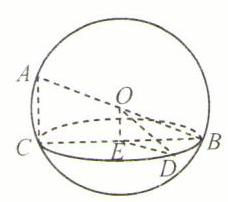
\includegraphics[width=0.2\textwidth]{bodyxb/src/bo_d20aucref24c73anc48g_221_1207_1858_228_202_0.jpg}
\end{center}


(第 251 题)

(1)求证:平面 ${ACB} \bot  \alpha$ ；

(2)设 ${AB}$ 与 $\alpha$ 所成角为 $\theta$ ,过球半径 ${OD}$ 且垂直于 $\alpha$ 的截面截弦 ${BC}$ 于点 $E$ ,求 $\bigtriangleup {OED}$ 与经过点 $O,D$ 的截面面积之比,并求 $\theta$ 为何值时, 面积之比最大.
